%%%%%%%%%%%%%%%%%%%%%%%%%%%%%%%%%%%%%%%%%%%%%%%%%%%%%%%%%%%%%%%%%%%%%%%%%%%%%%%%
% Template for USENIX papers.
%
% History:
%
% - TEMPLATE for Usenix papers, specifically to meet requirements of
%   USENIX '05. originally a template for producing IEEE-format
%   articles using LaTeX. written by Matthew Ward, CS Department,
%   Worcester Polytechnic Institute. adapted by David Beazley for his
%   excellent SWIG paper in Proceedings, Tcl 96. turned into a
%   smartass generic template by De Clarke, with thanks to both the
%   above pioneers. Use at your own risk. Complaints to /dev/null.
%   Make it two column with no page numbering, default is 10 point.
%
% - Munged by Fred Douglis <douglis@research.att.com> 10/97 to
%   separate the .sty file from the LaTeX source template, so that
%   people can more easily include the .sty file into an existing
%   document. Also changed to more closely follow the style guidelines
%   as represented by the Word sample file.
%
% - Note that since 2010, USENIX does not require endnotes. If you
%   want foot of page notes, don't include the endnotes package in the
%   usepackage command, below.
% - This version uses the latex2e styles, not the very ancient 2.09
%   stuff.
%
% - Updated July 2018: Text block size changed from 6.5" to 7"
%
% - Updated Dec 2018 for ATC'19:
%
%   * Revised text to pass HotCRP's auto-formatting check, with
%     hotcrp.settings.submission_form.body_font_size=10pt, and
%     hotcrp.settings.submission_form.line_height=12pt
%
%   * Switched from \endnote-s to \footnote-s to match Usenix's policy.
%
%   * \section* => \begin{abstract} ... \end{abstract}
%
%   * Make template self-contained in terms of bibtex entires, to allow
%     this file to be compiled. (And changing refs style to 'plain'.)
%
%   * Make template self-contained in terms of figures, to
%     allow this file to be compiled.
%
%   * Added packages for hyperref, embedding fonts, and improving
%     appearance.
%
%   * Removed outdated text.
%
%%%%%%%%%%%%%%%%%%%%%%%%%%%%%%%%%%%%%%%%%%%%%%%%%%%%%%%%%%%%%%%%%%%%%%%%%%%%%%%%

\documentclass[letterpaper,twocolumn,10pt]{article}
\usepackage{usenix-2020-09}

% to be able to draw some self-contained figs
\usepackage{tikz}
\usepackage{amsmath}

\usepackage{filecontents}
\usepackage{graphicx}
\usepackage{amsthm}
\usepackage{amssymb}
\usepackage{thmtools}
\usepackage{color}
\usepackage{enumitem}
\usepackage{bm}

\usepackage[linesnumbered, lined, boxed]{algorithm2e}

\usepackage[normalem]{ulem}

\newtheorem{definition}{Definition}
\newtheorem{theorem}{Theorem}
\newtheorem{lemma}{Lemma}
\newtheorem{proposition}{Proposition}
\newtheorem{corollary}{Corollary}
\newtheorem{remark}{Remark}

\SetKwInput{KwData}{Input}
\SetKwInput{KwResult}{Output}

\def\calA{\mathcal{A}}
\def\calB{\mathcal{B}}
\def\calC{\mathcal{C}}
\def\calD{\mathcal{D}}
\def\calE{\mathcal{E}}
\def\calF{\mathcal{F}}
\def\calG{\mathcal{G}}
\def\calH{\mathcal{H}}
\def\calI{\mathcal{I}}
\def\calJ{\mathcal{J}}
\def\calK{\mathcal{K}}
\def\calL{\mathcal{L}}
\def\calM{\mathcal{M}}
\def\calN{\mathcal{N}}
\def\calO{\mathcal{O}}
\def\calP{\mathcal{P}}
\def\calQ{\mathcal{Q}}
\def\calR{\mathcal{R}}
\def\calS{\mathcal{S}}
\def\calT{\mathcal{T}}
\def\calU{\mathcal{U}}
\def\calV{\mathcal{V}}
\def\calW{\mathcal{W}}
\def\calX{\mathcal{X}}
\def\calY{\mathcal{Y}}
\def\calZ{\mathcal{Z}}
\def\E{\mathbb{E}}
\def\R{\mathbb{R}}
\def\Z{\mathbb{Z}}
\def\hsbm{\textnormal{HSBM}}
\def\dpcom{\textsf{DPCommunity}}
\def\dphchsbm{\textsf{DPClusterHSBM}}
\def\dphcblocks{\textsf{DPHCBlocks}}
\def\sparsecut{\textsf{SparseCut}}
\def\linkage{\textsf{Linkage}}
\newcommand{\leaves}[1]{\texttt{leaves}(#1)}

\def\dcost{\textnormal{cost}}
\def\mwcost{\textnormal{rev}}
\def\cost{\omega}
\def\mw{\textsf{MW}}
\def\DPCut{\textnormal{DPCut}}
\def\edgewgt{\textnormal{edge-wgt}}
\def\bcutcost{\textnormal{bcut-cost}}
\newcommand{\cut}[1]{\|#1\|_{\textnormal{cut}}}

%TODO Fix these
\def\citep{\cite}
\def\citet{\cite}

\newtheorem{lem}{Lemma}
\newtheorem{obs}{Observation}

%\newcommand{\Jnote}[1]{\textcolor{red}{Jacob: #1}}
%\newcommand{\Anote}[1]{\textcolor{red}{Ale: #1}}
%\newcommand{\Vnote}[1]{\textcolor{red}{Vincent: #1}}
%\newcommand{\Mnote}[1]{\textcolor{red}{Mohammed: #1}}


\usepackage{hyperref}
\newcommand{\footremember}[2]{%
    \thanks{#2}
    \newcounter{#1}
    \setcounter{#1}{\value{footnote}}%
}
\newcommand{\footrecall}[1]{%
    \footnotemark[\value{#1}]%
}

\hypersetup{
  colorlinks,
  linkcolor={black},
  citecolor={red!70!black},
  urlcolor={blue!70!black}
}

% Switch conference/arXiv versions
\newif\ifconferenceon\conferenceonfalse
%\newif\ifconferenceon\conferenceontrue
\ifconferenceon
\newcommand{\conference}[1]{#1}
\newcommand{\arxiv}[1]{}
\else
\newcommand{\conference}[1]{}
\newcommand{\arxiv}[1]{#1}
\usepackage{balance}
\fi

% \pagestyle{empty}

%-------------------------------------------------------------------------------
\begin{document}
%-------------------------------------------------------------------------------

% %don't want date printed
% \date{}

% make title bold and 14 pt font (Latex default is non-bold, 16 pt)
\title{\Large \bf Communication-Efficient Triangle Counting under Local Differential Privacy}
% \thanks{This study was supported in part by JSPS KAKENHI JP19H04113.}}

\author{
{\rm Jacob Imola}\footremember{contributions}{The first and second authors made equal contribution.}\\
UC San Diego
\and
{\rm Takao Murakami}\footrecall{contributions}\\
AIST
\and
{\rm Kamalika Chaudhuri}\\
UC San Diego
} % end author

\maketitle

%-------------------------------------------------------------------------------
\begin{abstract}
%-------------------------------------------------------------------------------

Triangle counting in networks under LDP (Local Differential Privacy) is a fundamental task for analyzing connection patterns or calculating a 
clustering coefficient while strongly protecting sensitive friendships from a central server. In particular, a recent study proposes an algorithm
for this task that uses two rounds of interaction between users and the server to significantly reduce estimation error. However,
this algorithm suffers from a prohibitively 
% large 
high 
communication cost due to a large noisy graph each user needs to download.

% In this work, we propose triangle counting algorithms under LDP with a small estimation error and small communication cost. This is achieved by
% two algorithmic techniques -- an asymmetric version of randomized response, coupled with selective edge sampling and a double-clipping technique. 
% Through comprehensive evaluations, we show that our algorithms reduce the communication cost by a factor of more than 3600 while retaining the
% same estimation error. 

% Triangle counting in graphs under LDP (Local Differential Privacy) has been studied to analyze connection patterns or to calculate a clustering coefficient while strongly protecting sensitive friendships even from a central server.
% % Triangle counting in graph data is a fundamental task
% % A triangle count in graph data is one of the most basic subgraph counts useful, e.g., for calculating a clustering coefficient.
% % or constructing graph models.
% % To strongly protect sensitive friendship information even from a central server,
% % it is desirable to use
% % some studies adopt
% % LDP (Local Differential Privacy) as a privacy metric.
% % Some studies propose triangle counting algorithms under LDP (Local Differential Privacy) to
% % strongly protect sensitive friendship information even from a central server.
% In particular, a recent study shows that
% % the estimation error is significantly reduced by introducing an additional round between users and the server.
% although
% algorithms with one round of interaction between users and the server suffer from a very large estimation error,
% % and that
% the error is significantly reduced by introducing an additional round.
% % However, existing algorithms suffer from either a prohibitively large estimation error
% % due to a single round of interaction between users and the server
% % or prohibitively large communication cost
% % due to a large noisy graph each user needs to download at an additional round.
% % , hence unpractical for a large graph.
% % However,
% Their two-rounds algorithm however suffers from a prohibitively large communication cost
% due to a large noisy graph each user needs to download.
% % at the second round.
% % because each user needs to download a large noisy graph at the additional round.
% % Thus, they cannot be

In this work, we propose triangle counting algorithms under LDP with a small estimation error and communication cost.
We first
% show that simply sampling edges in the noisy graph results in a large estimation error
propose two-rounds algorithms
consisting of edge sampling and carefully selecting edges each user downloads
% that sample noisy edges and then carefully select noisy edges each user downloads
so that the estimation error is small.
Then we propose
a double clipping technique,
which clips the number of edges and then the number of noisy triangles,
% a combination of
% edge clipping and noisy triangle clipping,
% which we call double clipping,
to significantly reduce the sensitivity of each user's query.
Through comprehensive evaluation, we 
% We comprehensively evaluate our algorithms using two real datasets, and
% Our experimental results
show that our algorithms dramatically reduce the communication cost
% when compared with
of the existing algorithm, e.g., from
% 400 Gbits to 100 Mbits
6 hours to 8 seconds or less at a 20 Mbps download rate, while keeping
a small estimation error.
% the relative error much smaller than 1.
\end{abstract}

\section{Introduction}
\label{chap2-sec:intro}
Counting subgraphs (e.g., triangles, stars, cycles) is
% a fundamental task 
one of the most basic tasks 
for analyzing connection patterns
% for analyzing graph statistics
in
% a graph.
various graph data, e.g., social,
communication, and collaboration networks.
% , epidemiological networks.
% Graph statistics is important to understand the connection patterns in various graph data; e.g., social networks, collaboration networks,
% For example, a degree distribution in a social graph represents a distribution of the number of friends in the graph.
% A subgraph count (e.g.,
For example,
% a triangle count is the number of three nodes with three edges.
% A $k$-star count is the number of a node connected to $k$ other nodes.
a triangle is given by a set of three nodes with three edges, whereas a $k$-star is given by a central node connected to $k$ other nodes.
% a set of $k$ nodes connected a central node.
These subgraphs
% are important because they can be used to calculate
play a crucial role in calculating
a \textit{clustering coefficient} ($=\frac{3 \times \text{\#triangles}}{\text{\#2-stars}}$) (see Figure~\ref{chap2-fig:triangles_stars}). 
% which 
The clustering coefficient 
measures the average probability that
two friends of a user will also be a friend
% a friend's friend is also a friend
in a social graph \cite{Newman_PRL09}. 
Therefore, it is useful for measuring the effectiveness of friend suggestions. 
In addition, the clustering coefficient represents the degree to which users tend to cluster together. 
Thus, if it is large in some services/communities, we can effectively apply social recommendations \cite{Kolluri_CCS21} to the users. 
% for an example of
% the triangle and $k$-star counts and clustering coefficient).
% these subgraph counts).
% \cite{Newman_PRL09}.
% It is also known that these subgraphs are sufficient statistics for exponential random graph models
Triangles 
and $k$-stars 
% can also be used for
are also useful for 
% modeling graphs \cite{Jorgensen_SIGMOD16,Robins_SN07}.
% generating graphs based on some
constructing
graph models
\cite{Robins_SN07,Jorgensen_SIGMOD16}; 
% and other applications \cite{Imola_USENIX21}.
% (e.g., exponential random graph models \cite{Robins_SN07}, TriCycle \cite{Jorgensen_SIGMOD16}).
% Applications of triangle counting are summarized in \cite{Tsourakakis_JGAA11}. 
see also \cite{Tsourakakis_JGAA11} for other applications of triangle counting. 
However, graph data often involve sensitive data such as sensitive edges (friendships),
% that a user wants to keep secret,
% which 
and they 
can be leaked from 
% exact values of triangle counts and $k$-star counts \cite{Imola_USENIX21}.
exact numbers of triangles and $k$-stars \cite{Imola_USENIX21}.
% Therefore,
% there is a need for
% we need to develop an algorithm for
% counting
% subgraphs while strongly protecting user privacy.
% , which is the focus of this paper.


To analyze subgraphs while protecting user privacy, DP (Differential Privacy) \cite{DP} has been widely adopted as a privacy metric \cite{Ding_TKDE21,Imola_USENIX21,Karwa_PVLDB11,Sun_CCS19,Ye_ICDE20,Ye_TKDE21,Zhang_SIGMOD15}.
DP protects user privacy against adversaries with arbitrary background knowledge and is known as a gold standard for data privacy.
% Most studies on private graph analysis \cite{Chen_PoPETs20,Day_SIGMOD16,Hay_ICDM09,Karwa_PVLDB11,Kasiviswanathan_TCC13,Nissim_STOC07,Raskhodnikova_arXiv15,Song_arXiv18} assumes central DP
According to the underlying model, DP can be categorized into \textit{central (or global) DP} and \textit{LDP (Local DP)}.
Central DP assumes a scenario where
% that
a central server has personal data of all users.
% whereas LDP does not assume such trusted servers.
Although accurate analysis of subgraphs is possible under
% central DP
this model \cite{Ding_TKDE21,Karwa_PVLDB11,Zhang_SIGMOD15}, there is a risk that the entire graph is leaked from the server by illegal access or internal fraud \cite{data_breach2021,CambridgeAnalytica}.
In addition, central DP cannot be applied to  \textit{decentralized social networks} 
\cite{Diaspora,Mastodon,Minds,Paul_CN14} 
% \cite{Diaspora,Mastodon,Paul_CN14} 
% (e.g., Diaspora \cite{Diaspora}, Mastodon \cite{Mastodon}) 
% which has no central server that has the entire graph, and uses many servers each of which has personal data of users who have registered
where the entire graph is distributed across many servers. 
% nor 
We can even consider 
\textit{fully decentralized applications} where a server does not have
any original edge, 
% between users, 
% information about the original edges;
% For example,
% mobile application in which each user sends the number of her friends
e.g., a mobile app that sends a noisy degree (noisy number of friends) to the server, which then estimates a degree distribution. 
Central DP cannot be used in such applications. 

In contrast, LDP assumes a scenario where each user obfuscates her personal data (friends list in 
the case of graphs) 
% data) 
by herself and sends the obfuscated data to a possibly malicious server; i.e., it does not assume trusted servers.
Thus, it does not suffer from a data breach and can also be applied to the decentralized applications. 
% explained above.
% LDP does not assume trusted servers, hence
% can be applied to the above decentralized applications.
% In LDP, each user obfuscates her personal data (friends list in the case of graph data) by herself, and sends the obfuscated data to a (possibly malicious) server.
% Since the server does not have the original data, it does not suffer from the data breach.
LDP has been widely studied in tabular data where each row corresponds to a user's personal data (e.g., age, browser setting, location) 
\cite{Acharya_AISTATS19,Bassily_NIPS17,Erlingsson_CCS14,Kairouz_ICML16,Murakami_USENIX19,Wang_USENIX17} 
% \cite{Acharya_AISTATS19,Bassily_NIPS17,Erlingsson_CCS14,Fanti_PoPETs16,Kairouz_ICML16,Murakami_USENIX19,Qin_CCS16,Wang_USENIX17}, 
and also in graph data \cite{Imola_USENIX21,qin2017generating,Ye_ICDE20,Ye_TKDE21}.
For example, $k$-star counts can be very accurately estimated under LDP because each user can count $k$-stars of which she is a center and sends a noisy version of her $k$-star count to the server \cite{Imola_USENIX21}.

However, more complex subgraphs such as triangles are much harder to count under LDP because each user
% is not aware of
cannot see
edges between other users.
For example, in Figure~\ref{chap2-fig:triangles_stars}, user $v_1$ cannot see
% an edge between $v_2$ and $v_3$,
edges between $v_2$, $v_3$, and $v_6$ 
and therefore 
% , hence 
cannot count triangles involving $v_1$.
Thus,
% when only one-round interaction is allowed between each user and the server,
% instead of sending a noisy triangle count,
existing algorithms \cite{Imola_USENIX21,Ye_ICDE20,Ye_TKDE21}
% send noisy edges (rather than noisy triangle counts) obtained by randomized response \cite{Warner_JASA65} to a server.
obfuscate each user's edges (rather than her triangle count) by
% Warner's
RR (Randomized Response)
% randomized response
\cite{Warner_JASA65} and send noisy edges to a server.
% , which then estimates the triangle count.
% \cite{Imola_USENIX21,Ye_ICDE20,Ye_TKDE21} apply Warner's RR (Randomized Response) \cite{Warner_JASA65}, which flips 0/1 with some probability, to each edge and then estimate the triangle count.
Consequently, the server suffers from a
% very
prohibitively
large estimation error
% as shown in \cite{Imola_USENIX21} and Appendix~\ref{chap2-sec:one-round} in our paper 
(e.g., relative error $> 10^2$ in large graphs, 
as shown in Appendix~\ref{chap2-sec:one-round}) 
% (e.g., relative error $> 10^2$ in large graphs, as shown in Appendix~\ref{chap2-sec:one-round} of our paper)
because all three edges are noisy in any noisy triangle the server sees.

\begin{figure}[t]
  \centering
  
\includegraphics[width=0.85\linewidth]{fig/triangles_stars.pdf}
  
  \caption[Triangles, $2$-stars, and clustering coefficient.]{Triangles, $2$-stars, and clustering coefficient.}
  \label{chap2-fig:triangles_stars}
\end{figure}

A recent study \cite{Imola_USENIX21} shows that the estimation error in
% triangle counting under LDP
locally private triangle counting
is significantly reduced by introducing an additional round of interaction between users and the server.
Specifically, if the server publishes the noisy graph (all noisy edges) sent by users at the first round, then each user can count her noisy triangles such that \textit{only one edge} is noisy (as she knows two edges connected to her).
Thus,
% each user
the algorithm in \cite{Imola_USENIX21} sends each user's noisy triangle count (with additional noise) to the server at the second round.
Then the server can accurately estimate the triangle count. 
% between users and the server 
% The algorithm in \cite{Imola_USENIX21} 
This algorithm also requires a much smaller number of interactions 
% between users and the server 
(i.e., only two) than collaborative approaches \cite{Kairouz_FTML21,Shokri_CCS15} that generally require many interactions. 

Unfortunately, 
% this algorithm 
the algorithm in \cite{Imola_USENIX21} 
is still
% far from practical
impractical 
for a large-scale graph.
% as shown in this paper.
Specifically, the noisy graph sent by users is dense, hence extremely large for a large-scale graph, e.g.,
$500$
% $400$
Gbits for a graph of
% about $900000$ users, as in our experiments).
a million users.
The problem is that \textit{every user} needs to download such huge data; e.g., when the download speed is $20$ Mbps (which is a recommended speed in YouTube \cite{YouTube_speed}), every user needs about 7 hours to download the noisy graph.
Since the communication ability might be limited for some users, the algorithm in \cite{Imola_USENIX21} cannot be
% applied to
used for
% a large-scale graph with diverse communication environments.
applications with large and diverse users.

In summary, existing triangle algorithms under LDP suffer from either a prohibitively large estimation error or a prohibitively 
% large 
high 
communication cost.
% For the same reason, they cannot calculate the clustering coefficient
They also suffer from the same issues when calculating the clustering coefficient.

% \colorB{
% \begin{itemize}
%     \item graph statistics; e.g., degree distribution, subgraph count (e.g., 2-stars, triangles), clustering coefficient.
%     \item privacy issue, DP, central DP, LDP.
%     \item 2-star counting under LDP is easy because...
%     \item triangle counting (hence clustering coefficient) is much harder because...
%     \item Previous work \cite{Imola_USENIX21}. Communication cost is prohibitively large (e.g., 400 Gbits for \IMDB{}).
%     \item This work
% \end{itemize}}

\smallskip
\noindent{\textbf{Our Contributions.}}~~We 
% In this work, we 
propose locally private triangle counting algorithms with a small estimation error and small communication cost.
% dramatically reduce the communication cost in accurate two-rounds triangle counting under LDP
% introduce some novel algorithms
% dramatically reduce the communication cost in locally private triangle counting
% address this issue
% by introducing some novel algorithms.
% Specifically, our contributions are:
Our contributions are as follows:

\begin{itemize}
    \item We propose two-rounds triangle algorithms
% that sample edges and then select edges each user downloads.
consisting of \textit{edge sampling} after RR and \textit{selecting edges each user downloads}.
In particular, we show that a simple extension of \cite{Imola_USENIX21} with edge sampling suffers from a large estimation error for a large or dense graph where the number of 4-cycles (such as $v_1$-$v_2$-$v_3$-$v_6$-$v_1$
% and $v_4$-$v_5$-$v_7$-$v_6$-$v_4$
in Figure~\ref{chap2-fig:triangles_stars}) is large.
To address this issue, we propose some strategies for selecting edges to download to reduce the error caused by the 4-cycles, which we call the \textit{4-cycle trick}.
\item We
show that
% the above algorithms
the algorithms with the $4$-cycle trick
still suffer from a large estimation error due to
% a large global sensitivity
% a large amount of the Laplacian noise.
large Laplacian noise for each user.
% To address this, 
To significantly reduce the Laplacian noise, 
we
propose a \textit{double clipping} technique,
which clips 
a degree (the number of edges) of each user 
% the number of edges 
with LDP and then clips the number of noisy triangles. 
% to significantly reduce the Laplacian noise.
% which significantly reduces the Laplacian noise by edge clipping and noisy triangle clipping.
% consists of edge clipping and noisy triangle clipping, to significantly reduce the global sensitivity in DP \cite{DP}.
% consisting of edge clipping and noisy triangle clipping
\item We evaluate our algorithms using two real datasets.
We show that our entire algorithms with the 4-cycle trick and double clipping
% provide the best performance, and
dramatically reduce the communication cost
% when compared with
of
\cite{Imola_USENIX21}.
For example,
% when the number of users is about $900000$,
for a graph with about $900000$ users,
we reduce the download cost from $400$ Gbits ($6$ hours when $20$ Mbps) to 
% $100$ Mbits ($5$ seconds) 
$160$ Mbits ($8$ seconds) or less 
while keeping the relative error much smaller than 1.
\end{itemize}
Thus, locally private triangle counting is now much more practical. 
% Note that the number of interactions between users and a server in our algorithms (i.e, only two) is also much smaller than collaborative approaches that generally requires a number of interactions. 
In Appendix~\ref{chap2-sec:cluster}, we also show that we can estimate the clustering coefficient with a small estimation error and download cost. 
For example, our algorithms are useful for measuring the effectiveness of friend suggestions or social recommendations in decentralized 
social networks, 
% SNS, 
e.g., Diaspora \cite{Diaspora}, Mastodon \cite{Mastodon}. 
% We published
Our source code
% with C/C++
is available at 
\cite{TriangleLDP}. 
%\cite{ComTriLDP}.
% as open-source software.

All the proofs of our privacy and utility analysis 
% The proofs of all statements 
are given in \conference{the full version \cite{Imola_arXiv22}}\arxiv{Appendices~\ref{chap2-sec:proof_seq_comp_edge_LDP}, \ref{chap2-sec:proof_algorithms}, and \ref{chap2-sec:proof_double_clip}}.

\smallskip
\noindent{\textbf{Technical Novelty.}}~~Below we explain more about 
% also clarify 
the technical novelty of this paper. 
Although we focus on two-rounds local algorithms in the same way as \cite{Imola_USENIX21}, we introduce several new algorithmic ideas previously unknown in the literature. 

First, our 4-cycle trick is totally new. 
Although some studies focus on 4-cycle counting \cite{Bera_STACS17,Kallaugher_PODS19,Manjunath_ESA11,McGregor_PODS20}, this work is the first to use 4-cycles to improve communication efficiency. 
Second, selective download of parts of a centrally computed quantity is also new. 
This is not limited to graphs -- even in machine learning, 
% or federated learning, 
there are no such strategic download techniques previously, to our knowledge. 
Third, our utility analysis of our 
% two-rounds 
triangle 
algorithms (Theorem~\ref{chap2-thm:l2loss_algorithms}) is 
% also now because it 
different from \cite{Imola_USENIX21} in that ours introduces subgraphs such as 4-cycles and $k$-stars. 
This leads us to our 4-cycle trick. 
Fourth, we propose two triangle algorithms that introduce the 4-cycle trick and show that the more tricky one provides the best performance because of 
its low sensitivity in DP.
% small Laplacian noise. 

% Fourth, 
Finally, 
our double clipping is new. 
Andrew \textit{et al.} \cite{Andrew_NeurIPS21} propose an adaptive clipping technique, which applies clipping twice. 
However, they focus on federated averaging, 
% or SGD (Stochastic Gradient Descent), 
and their problem setting is different from our graph setting. 
In particular, they require a private quantile of the norm distribution. 
In contrast, we need only a much simpler estimate: a private degree. 
Here, we use the fact that the degree has a small sensitivity (sensitivity $=1$) in DP for edges. 
We also provide a new, reasonably tight bound on the probability that the noisy triangle count exceeds a clipping threshold (Theorem~\ref{chap2-thm:triangle_excess}). 
Thanks to the two differences, we obtain a significant communication improvement: two or three orders of magnitude. 

% Finally, we show an interesting finding when we combine the 4-cycle trick and double clipping. 
% Specifically, we propose two triangle algorithms that introduce the 4-cycle trick and show that the more tricky one provides the best performance because of its low sensitivity.

\section{Related Work}
\label{chap2-sec:related}
% !TEX root=main.tex
\noindent{\textbf{Triangle Counting.}}~~Triangle
% We finally note that triangle
counting has been extensively studied in a non-private setting \cite{Bera_KDD20,Bera_PODS20,Chu_KDD11,Eden_FOCS15,Seshadhri_SDM13,Suri_WWW11,Tsourakakis_KDD09,Wu_TKDE16} 
% \cite{Arifuzzaman_CIKM13,Bera_KDD20,Bera_PODS20,Chu_KDD11,Eden_FOCS15,Kolountzakis_IM12,Seshadhri_SDM13,Suri_WWW11,Tangwongsan_CIKM13,Tsourakakis_KDD09,Wu_TKDE16}
(it is almost a sub-field in itself)
because it requires high time complexity for large graphs.

Edge sampling \cite{Bera_PODS20,Eden_FOCS15,Tsourakakis_KDD09,Wu_TKDE16} is one of the most basic techniques to improve 
% the 
scalability.
Although edge sampling is simple, it is quite effective -- it is reported in \cite{Wu_TKDE16} that edge sampling outperforms other sampling techniques such as node sampling and triangle sampling.
Based on this, we adopt edge sampling after RR\footnote{We also note that a study in \cite{Nguyen_TDP16} proposes a graph publishing algorithm in the central model that independently changes 1-cells (edges) to 0-cells (no edges) with some probability and then 
changes a fixed number of 0-cells to 1-cells \textit{without replacement}. 
However, each 0-cell is \textit{not} independently sampled in this case, and consequently, 
their proof that relies on the independence of the noise to each 0-cell is incorrect. 
In contrast, our algorithms provide DP because we apply sampling after RR, i.e., post-processing.} 
with new techniques such as the 4-cycle trick and double clipping.
% to significantly improve
Our entire algorithms significantly improve the communication cost, as well as the space and time complexity, under LDP (see Sections~\ref{chap2-sub:clip_theoretical_analysis}
and \ref{chap2-sec:experiments}).
% for details).
% to significantly improve the communication cost, as well as the space and time complexity, under LDP (see Section~\ref{chap2-sub:clip_theoretical_analysis} for the performance of our entire algorithms).

\smallskip
\noindent{\textbf{DP on Graphs.}}~~For private graph analysis, DP has been widely adopted as a privacy metric.
Most of them adopt central (or global) DP
\cite{Day_SIGMOD16,Ding_TKDE21,Hay_ICDM09,Karwa_PVLDB11,Kasiviswanathan_TCC13,Raskhodnikova_arXiv15,Zhang_SIGMOD15}, 
% \cite{Chen_PoPETs20,Day_SIGMOD16,Ding_TKDE21,Hay_ICDM09,Kasiviswanathan_TCC13,Raskhodnikova_arXiv15,Song_arXiv18,Wang_TDP13,Wang_PAKDD13,Zhang_SIGMOD15}, 
which suffers from the data breach issue.
% explained above.
% in which the original graph might be leaked from the server by illegal access.

LDP on graphs has recently studied in some studies, e.g., synthetic data generation \cite{Qin_CCS17}, subgraph counting \cite{Imola_USENIX21,Sun_CCS19,Ye_ICDE20,Ye_TKDE21}.
% Sun \textit{et al.}
A study in
\cite{Sun_CCS19} proposes subgraph counting algorithms in a setting where each user
% can see all of her friends' friends.
allows her friends to see all her connections.
% However, it cannot be applied to many applications that do not allow friends to see
% Although each user can count her triangles at the first round in this setting,
However, this setting is unsuitable for
% it cannot be applied to
many applications; e.g., in Facebook, a user can easily change her setting so that
% her friend cannot see the other friends.
her friends cannot see her connections.



Thus, we consider a model where each user can see only her friends.
% , as in \cite{Sun_CCS19,Ye_ICDE20,Ye_TKDE21}.
In this model, some one-round algorithms \cite{Ye_ICDE20,Ye_TKDE21}
and two-rounds algorithms\cite{Imola_USENIX21} have been proposed.
However, they suffer from a prohibitively large estimation error or high communication cost, as explained in Section~\ref{chap2-sec:intro}.

% Recently proposed network LDP protocols \cite{Cyffers_arXiv21} consider, instead of a central server, collecting private data with user-to-user communication protocols along a graph. 
% Their results apply to sums, histograms, and SGD. 
% In our setting, we instead compute graph statistics with a central server.
% Thus, their use of graphs is orthogonal to ours. 
% The same applies to 
% another work \cite{Sabater_arXiv21} 
% that improves 
% the utility of an averaging query
% by correlating the noise of users according to a graph.
Recently proposed network LDP protocols \cite{Cyffers_arXiv21} consider, instead of a central server, collecting private data with user-to-user communication protocols along a graph. 
They focus on sums, histograms, and SGD (Stochastic Gradient Descent) and do not provide subgraph counting algorithms. 
Moreover, they focus on hiding each user's private dataset rather than hiding an edge in a graph. 
Thus, their approach cannot be applied to our task of subgraph counting under LDP for edges. 
% In our setting, we instead compute graph statistics with a central server.
% Thus, their use of graphs is orthogonal to ours. 
The same applies to 
another work \cite{Sabater_arXiv21} 
that improves 
the utility of an averaging query
by correlating the noise of users according to a graph.

\smallskip
\noindent{\textbf{LDP.}}~~RR~\cite{Kairouz_ICML16,Warner_JASA65} 
% Randomized response
and 
RAPPOR~\cite{Erlingsson_CCS14} 
% RAPPOR~\cite{Erlingsson_CCS14, Fanti_PoPETs16} 
have been widely used 
% to perform a wide range of tasks 
for tabular data 
in 
% local DP. 
LDP. 
Our work uses RR in part of our algorithm but
builds off of it significantly. One noteworthy result in this area is HR (Hadamard Response) \cite{Acharya_AISTATS19}, which is state-of-the-art for tabular data
and requires low communication. However, this result is not applied to graph
data and does not address the communication issues considered in this paper.
Specifically, applying HR to each bit in a neighbor list will result in 
% $O(n)$ communication cost 
$O(n^2)$ ($n$: \#users) download cost 
in the same way as 
the previous work \cite{Imola_USENIX21} that uses RR. 
% previous work in private, local graph
% statistics~\cite{Imola_USENIX21} does. 
Applying HR to an entire neighbor list
(which has $2^n$ possible values) will similarly result in 
% $O(\log 2^n) = O(n)$
% communication.
$O(n \log 2^n) = O(n^2)$ download cost. 

Previous work on distribution estimation~\cite{Kairouz_ICML16,Murakami_USENIX19,Wang_USENIX17} or 
% heavy hitters \cite{Bassily_NIPS17} 
heavy hitters \cite{Bassily_NIPS17} 
addresses a different problem than ours, as they assume that every user has
i.i.d. 
(independent and identically distributed) 
samples. 
In our setting, a user's neighbor list is non-i.i.d. (as one edge is shared by two users), 
% user data is an arbitrary graph, 
which does not
fit into their statistical framework.

% In work on heavy hitters in the local DP model \cite{Bassily_NIPS17,Qin_CCS16},
% each user holds a domain element and frequencies of domain elements are computed
% privately. While previous work considers user and server communication and computation
% costs as we do, their problem is not very related to our setting of graph statistics.

%\commentTM{About HR \cite{Acharya_AISTATS19}:
%Although HR is a state-of-the-art in tabular data, it is not applied to graph data and does not address the communication issue considered in this paper. For example, the communication complexity of HR (=log k) is the same as that of k-RR  (=log k), where k is category size (Table 2 in [8]). Thus,
%- if we apply HR to each bit of neighbor list, it suffers from high communication cost in the same way as our USENIX paper that uses RR.
%- if we apply HR to the whole neighbor list (n-dim vector = $2^n$ categorical data), the communication cost is high (=log $2^n$ = n).}

 %-------------------------------------------------------------------------------
\section{Preliminaries}
%-------------------------------------------------------------------------------
\label{chap1-sec:preliminaries}

% \subsection{Notations and Graphs}
% \label{chap1-sub:notations}
% \subsection{Graphs and Centralized Differential Privacy}
\subsection{Graphs and Differential Privacy}
\label{chap1-sub:graphs_CDP}
\noindent{\textbf{Graphs.}}~~Let $\nats$, $\nnints$, $\reals$, and $\nnreals$ be the sets of natural numbers, non-negative integers, real numbers, and non-negative real numbers, respectively. 
For $a \in \nats$, let $[a] = \{1, 2, \ldots, a\}$. 

We consider an undirected graph $G=(V,E)$, where 
$V$ is a set of nodes (i.e., users) and $E$ is a set of edges. 
Let $n \in \nats$ be the number of users in $V$, and let $v_i \in V$ the $i$-th user; i.e., $V=\{v_1,\ldots,v_n\}$. 
An edge $(v_i, v_j) \in E$ represents a relationship between users $v_i \in V$ and $v_j \in V$. 
% a node $v \in V$ represents a user and an edge $(u,v) \in E$ represents a relationship
% between users $u \in V$ and $v \in V$. 
The number of edges connected to a single node is called the \textit{degree} of the node. 
Let $d_{max} \in \nats$ be the \textit{maximum degree} (i.e., maximum number of edges connected to a node) in graph $G$. 
Let $\calG$ be the set of possible graphs 
% $G=(V,E)$ with $V=\{v_1,\ldots,v_n\}$. 
$G$ on $n$ users. 
A graph $G \in \calG$ can be represented as a symmetric adjacency matrix $\bmA=(a_{i,j}) \in \{0,1\}^{n \times n}$, where $a_{i,j}=1$ if $(v_i,v_j) \in E$ and $a_{i,j}=0$ otherwise.

% \subsection{Centralized Differential Privacy}
% \label{chap1-sub:CDP}
\smallskip
% \noindent{\textbf{Centralized DP.}}~~
\noindent{\textbf{Types of DP.}}~~
DP (Differential Privacy) \cite{DP,Dwork_ICALP06} is known as a gold standard for data privacy. 
According to the underlying architecture, DP can be divided into two 
% categories: 
types: 
\textit{centralized DP} and \textit{LDP (Local DP)}. 
% the one in the centralized (or global) model and the one in the local model. 
% In the centralized model, a trusted database 
Centralized DP assumes the centralized model, where a ``trusted'' data collector 
% database administrator 
collects the original personal data from all users and obfuscates a query (e.g., counting query, histogram query) on the set of personal data. 
% In contrast, 
LDP assumes the local model, where each user does not trust even the data collector. 
In this model, each user obfuscates a query on her personal data by herself and sends the obfuscated data to the data collector. 
% We begin by explaining centralized DP on graphs.

% There are two types of DP on graphs: 
If the data are represented as a graph, we can consider two types of DP: 
% centralized DP: 
% If the input is a graph, we can consider two types of DP: 
% centralized DP: 
% \textit{edge centralized DP} and \textit{node centralized DP} \cite{Hay_ICDM09}. 
\textit{edge DP} and \textit{node DP} \cite{Hay_ICDM09,Raskhodnikova_Encyclopedia16}. 
% We refer to edge DP and node DP in the centralized model as edge centralized DP and node centralized DP, respectively. 
Edge DP considers two neighboring graphs $G, G' \in \calG$ that differ in one edge. 
In contrast, node DP considers two neighboring graphs $G, G' \in \calG$ in which $G'$ is obtained from $G$ by adding or removing one node along with its adjacent edges. 
% Although node DP guarantees stronger privacy than edge DP, 
% it is much harder to attain. 

% Zhang \textit{et al.} \cite{Zhang_USENIX20} proposed an algorithm for software usage analysis with node DP in the local model, where a node represents a software component 
% and an edge represents a control-flow between components. 
% However, we consider a totally different problem, where each node represents a user (rather than a software component). 
Although Zhang \textit{et al.} \cite{Zhang_USENIX20} consider node DP in the local model where each node represents a software component, we consider a totally different problem where each node represents a user. 
% (rather than a software component). 
In the latter case, 
% achieving node DP in the local model is extremely difficult 
% because each user needs to hide the \textit{existence of herself} along with her all edges against the data collector. 
node DP requires us to hide the \textit{existence of each user} along with her all edges. 
% against the data collector. 
However, many applications in the local model send the identity of each user to a server. 
For example, 
we can consider a mobile application 
% that asks a users how many friends she met today and sends noisy counts and her user ID to a server. 
that sends to a server how many friends a user met today along with her user ID. 
In this case, the user may not mind sending her user ID, 
% (i.e., who the user is), 
but may want to hide her edge information (i.e., who she met today). 
Although we cannot use node DP in such applications, we can use edge DP to deny the presence/absence of each edge (friend). 
Thus we focus on edge DP in the same way as \cite{qin2017generating,Sun_CCS19,Ye_ICDE20,Ye_TKDE21}. 

% We refer to edge DP in the centralized model as \textit{edge centralized DP}, and explain it in detail below.
Below we explain edge DP in the centralized model. 

\smallskip
\noindent{\textbf{Centralized DP.}}~~We call edge DP in the centralized model \textit{edge centralized DP}. 
% Edge centralized DP is 
% Edge centralized DP considers two neighboring graphs that differ in one edge. 
Formally, it is defined as follows:

\begin{definition} [$\epsilon$-edge centralized DP] \label{chap1-def:edge_CDP} 
Let $\epsilon \in \nnreals$. 
A randomized algorithm $\calM$ with domain $\calG$ provides \emph{$\epsilon$-edge centralized DP} 
if for any two 
neighboring 
graphs $G, G' \in \calG$ that differ in one edge and any $S \subseteq \mathrm{Range}(\calM)$, 
\begin{align}
\Pr[\calM(G) \in S] \leq e^\epsilon \Pr[\calM(G') \in S].
\label{chap1-eq:edge_CDP}
\end{align}
\end{definition}
Edge centralized DP guarantees that an adversary who has observed the output of $\calM$ cannot determine whether it is come from $G$ or $G'$ with a certain degree of confidence. 
The parameter $\epsilon$ is called the \textit{privacy budget}. 
% and controls the amount of information leaked from the output of $\calM$. 
If $\epsilon$ is close to zero, then $G$ and $G'$ are almost equally likely, which means that an edge in $G$ is strongly protected. 

We also note that edge DP can be 
% easily extended 
used 
to protect $k\in\nats$ edges by using 
the notion of group privacy \cite{DP}.
Specifically, if $\calM$ provides $\epsilon$-edge centralized DP, then for any two graphs $G, G' \in \calG$ that differ in $k$ edges and any $S \subseteq \mathrm{Range}(\calM)$, we obtain: 
$\Pr[\calM(G) \in S] \leq e^{k\epsilon} \Pr[\calM(G') \in S]$; i.e., $k$ edges are protected with privacy budget $k\epsilon$.

\subsection{Local Differential Privacy}
\label{chap1-sub:LDP}
LDP (Local Differential Privacy) \cite{Kasiviswanathan_FOCS08,Duchi_FOCS13} is a privacy metric to protect personal data of each user in the local model. 
LDP has been originally introduced to protect each user's data record that is independent from the other records. 
However, in a graph, each edge is connected to two users. 
Thus, when we define edge DP in the local model, 
% i.e., \textit{edge LDP}, 
we should consider what we want to protect. 
In this paper, we consider two definitions of edge DP in the local model: \textit{edge LDP} in \cite{qin2017generating} and 
% \textit{entire edge LDP} 
\textit{relationship DP} 
introduced in this paper. 
Below, we will explain these two definitions in detail. 

% Applying LDP to a graph is not straightforward 
% because adding or removing one edge will affect neighbor lists of two users. 

\smallskip
\noindent{\textbf{Edge LDP.}}~~Qin \textit{et al.} \cite{qin2017generating} defined edge LDP based on a user's \textit{neighbor list}. 
% use the definition of edge LDP in \cite{qin2017generating}, which is based on a user's \textit{neighbor list}. 
Specifically, 
% given a user in $V$, 
% let $b_i \in \{0,1\}$ be a binary bit that takes $1$ if there is an edge between the user and user $v_i \in V$ and $0$ otherwise. 
% Let 
% $\bmb = (b_1, \ldots, b_n) \in \{0,1\}^n$ be a neighbor list. 
% Let $\bma_i = (a_{i,1}, \ldots, a_{i,n}) \in \{0,1\}^n$ be the $i$-th row of the adjacency matrix $\bmA$. 
% Note that a graph $G$ can be represented as neighbor lists $\textbf{a}_1, \ldots, \textbf{a}_n$, and $\bma_i$ is a neighbor list of user $v_i$. 
let $\bma_i = (a_{i,1}, \ldots, a_{i,n}) \in \{0,1\}^n$ be a neighbor list of user $v_i$. 
Note that $\bma_i$ is the $i$-th row of the adjacency matrix $\bmA$ of graph $G$. 
In other words, graph $G$ can be represented as neighbor lists $\textbf{a}_1, \ldots, \textbf{a}_n$. 

Then edge LDP is defined as follows: 

\begin{definition} [$\epsilon$-edge LDP \cite{qin2017generating}] \label{chap1-def:edge_LDP} 
Let $\epsilon \in \nnreals$. 
For any $i \in [n]$, let $\calR_i$ with domain $\{0,1\}^n$ be a randomized algorithm of user $v_i$. 
% A randomized algorithm $\calR$ with domain $\{0,1\}^n$ 
$\calR_i$ 
provides \emph{$\epsilon$-edge LDP} 
if for any two neighbor lists 
% $\bmb, \bmb' \in \{0,1\}^n$ 
$\bma_i, \bma'_i \in \{0,1\}^n$ 
that differ in one bit and any 
% $S \subseteq \mathrm{Range}(\calR)$, 
$S \subseteq \mathrm{Range}(\calR_i)$, 
\begin{align}
% \Pr[\calR(\bmb) \in S] \leq e^\epsilon \Pr[\calR(\bmb') \in S].
\Pr[\calR_i(\bma_i) \in S] \leq e^\epsilon \Pr[\calR_i(\bma'_i) \in S].
\label{chap1-eq:edge_LDP}
\end{align}
\end{definition}
Edge LDP in Definition~\ref{chap1-def:edge_LDP} protects 
a single bit in a neighbor list with privacy budget $\epsilon$. 
% For example, consider an application that asks a users how many friends she met today and sends noisy counts and her user ID to a server. 
% In this case, the user would not mind sending her identity 
% % (i.e., who the user is), 
% but want to hide who she met today (i.e., who are her neighbors). 
% Edge LDP can be used to deny the presence/absence of one neighbor.
As with edge centralized DP, edge LDP can also be 
% extended 
used 
to protect $k \in \nats$ 
bits in a neighbor list 
% neighbors 
by using group privacy; i.e., $k$ bits in a neighbor list are protected with privacy budget $k\epsilon$. 

% We can consider an application of the randomized algorithm $\calR$ with input $\bmb$ as follows. 
% For example, suppose that a data collector asks each user to send some query (e.g., number of friends, who are friends) on her neighbor list $\bmb$. 
% To protect $\bmb$, each user obfuscates her answer to the query by using $\calR$ and sends the noisy answer to the data collector. 
% Then the data collector estimates some graph statistics 
% (e.g., number of triangles, clustering coefficient) 
% based on the noisy answer from each user. 

\smallskip
% \noindent{\textbf{RNL (Randomized Neighbor List).}}~~
\noindent{\textbf{RR (Randomized Response).}}~~As a simple example of a randomized algorithm 
% $\calR$ 
$\calR_i$ 
providing $\epsilon$-edge LDP, we explain 
% the 
Warner's RR (Randomized Response) \cite{Warner_JASA65} applied to a neighbor list, 
which is called 
% the RNL (Randomized neighbor List) 
the randomized neighbor list in \cite{qin2017generating}. 
% and is also used in \cite{Ye_ICDE20}. 

Given a neighbor list 
% $\bmb \in \{0,1\}^n$, 
$\bma_i \in \{0,1\}^n$, 
% the RNL 
this algorithm 
outputs a noisy neighbor lists 
% $\bms = (s_1, \ldots, s_n) \in \{0,1\}^n$ 
$\bmb = (b_1, \ldots, b_n) \in \{0,1\}^n$ 
by flipping each bit in 
% $\bmb$ 
$\bma_i$ 
with probability $p = \frac{1}{e^\epsilon + 1}$; i.e., for each $j \in [n]$, 
% $s_i \neq b_i$ with probability $p$ and $s_i = b_i$ with probability $1-p$. 
$b_j \neq a_{i,j}$ with probability $p$ and $b_j = a_{i,j}$ with probability $1-p$. 
Since 
% $\Pr[\calR(\bmb) \in S]$ and $\Pr[\calR(\bmb') \in S]$ 
$\Pr[\calR(\bma_i) \in S]$ and $\Pr[\calR(\bma'_i) \in S]$ 
in (\ref{chap1-eq:edge_LDP}) differ by $e^\epsilon$ for 
% $\bmb$ and $\bmb'$ 
$\bma_i$ and $\bma'_i$ 
that differ in one bit, 
% It is easy to verify that 
% the RNL 
this algorithm 
provides $\epsilon$-edge LDP. 

\smallskip
% \noindent{\textbf{Remark.}}~~
% \noindent{\textbf{Alternative definition of edge LDP.}}~~
\noindent{\textbf{Relationship DP.}}~~In graphs such as social networks, 
% For graph datasets, 
it is usually the case that two users share knowledge of the presence of an edge between them. 
% For example, in social networks it is usually the norm that
% friendship status is known by both parties.
% With the goal of hiding their mutual edge, 
To hide their mutual edge, 
we must consider
that both user's outputs can leak information. 
We introduce a DP definition called relationship DP that hides \textit{one entire edge in graph $G$ during the whole process:}
% avoid confusion. 
% For example, divide a graph $G$ into disjoint sets $(G_1, \ldots, G_n)$ such that user $v_i$ can see $G_i$. 
% For example, 

% Then 
% We define relationship DP as follows: 
% (we call this version of edge LDP \textit{entire edge LDP} to avoid confusion):

\begin{definition} [$\epsilon$-relationship DP] 
% [$\epsilon$-entire edge LDP] 
\label{chap1-def:entire_edge_LDP} 
Let $\epsilon \in \nnreals$. 
% Let $\calR_1, \ldots, \calR_n$ be randomized algorithms, each of which is with domain $\{0,1\}^n$. 
A tuple of randomized algorithms $(\calR_1, \ldots, \calR_n)$, 
each of which is with domain $\{0,1\}^n$, 
provides 
% \emph{$\epsilon$-entire edge LDP} 
\emph{$\epsilon$-relationship DP} 
if for any two 
neighboring 
graphs $G, G' \in \calG$ that differ in one edge and any $S \subseteq \mathrm{Range}(\calR_1) \times \ldots \times \mathrm{Range}(\calR_n)$, 
\begin{align}
&\Pr[(\calR_1(\bma_1), \ldots, \calR_n(\bma_n)) \in S] \nonumber\\
&\leq e^\epsilon \Pr[(\calR_1(\bma'_1), \ldots, \calR_n(\bma'_n)) \in S],
\label{chap1-eq:entire_edge_LDP}
\end{align}
where $\bma_i$ (resp.~$\bma'_i$) $\in \{0,1\}^n$ is the $i$-th row of the adjacency matrix of graph $G$ (resp.~$G'$).
\end{definition}

Relationship DP is the same as \textit{decentralized DP} in \cite{Sun_CCS19} except that the former (resp.~latter) assumes that each user knows only her friends (resp.~all of her friends' friends).

% Relationship DP is distinct from edge LDP because 
Edge LDP assumes that 
% user $v_i$ being connected to user $v_j$ 
user $v_i$'s edge connected to user $v_j$ 
and 
% user $v_j$ being connected to user $v_i$ 
user $v_j$'s edge connected to user $v_i$ 
are different secrets, with user $v_i$ knowing the former and user $v_j$ knowing the latter. 
% As we stated above, the presence of an edge is usually known by both its users. 
Relationship DP assumes that the two secrets are the same.

% Since secrets are shared among two users, 
Note that 
the threat model of relationship DP is 
% not quite 
different from 
that of 
% local DP: 
LDP -- 
some amount of trust must be given to the other users 
in relationship DP. 
Specifically, user $v_i$ must trust user $v_j$ to not leak information
about their shared edge. If $k \in \nats$ users decide not to follow their protocols, 
then up to $k$ edges incident to user $v_i$ may be compromised. This trust model
is stronger than 
% local DP, 
LDP, 
which assumes nothing about what other users 
% may 
do,
but is much weaker than centralized DP in which 
% all information of a user is 
all edges are 
in the hands of the central party.

Other than the differing threat models, relationship DP and edge LDP are quite closely related:

\begin{proposition} \label{chap1-prop:edge_LDP_entire_edge_LDP} 
If randomized algorithms $\calR_1, \ldots, \calR_n$ provide $\epsilon$-edge LDP, 
then $(\calR_1, \ldots, \calR_n)$ provides $2\epsilon$-relationship DP.
\end{proposition}

\begin{proof}
The existence of edge $(v_i, v_j) \in E$ affects two elements $a_{i,j}, a_{j,i} \in \{0,1\}$ in the adjacency matrix $\bmA$. 
  Then by group privacy~\cite{DP}, Proposition~\ref{chap1-prop:edge_LDP_entire_edge_LDP} holds.
\end{proof}

% The existence of edge $(v_i, v_j) \in E$ affects two elements $a_{i,j}, a_{j,i} \in \{0,1\}$ in the adjacency matrix $\bmA$. 
% Therefore, by the composition theorem \cite{DP}, if all of the randomized algorithms $\calR_1, \ldots, \calR_n$ provide $\epsilon$-edge LDP in Definition~\ref{chap1-def:edge_LDP}, 
% then the tuple $(\calR_1, \ldots, \calR_n)$ provides $2\epsilon$-entire edge LDP in Definition~\ref{chap1-def:entire_edge_LDP}; i.e., the privacy budget is at most doubled. 

Proposition~\ref{chap1-prop:edge_LDP_entire_edge_LDP} states that when we want to protect one edge as a whole, the privacy budget is at most doubled. 
Note, however, that 
% the privacy budget is not changed for some randomized algorithms. 
some randomized algorithms do not have this doubling issue. 
For example, we can apply the RR to the $i$-th neighbor list $\bma_i$ so that $\calR_i$ outputs noisy bits 
% $(t_{i+1}, \ldots, t_n) \in \{0,1\}^{n-i}$ 
% $(t_1, \ldots, t_{i-1}) \in \{0,1\}^{i-1}$ 
$(b_1, \ldots, b_{i-1}) \in \{0,1\}^{i-1}$ 
for only users 
% $v_{i+1}, \ldots, v_n$ with larger user IDs; 
$v_1, \ldots, v_{i-1}$ with smaller user IDs; 
i.e., 
% In other words, we can modify the RNL as follows: 
for each 
% $j \in \{i+1, \ldots, n\}$, 
$j \in \{1, \ldots, i-1\}$, 
% $\calR_i$ outputs $(t_{i+1}, \ldots, t_n) \in \{0,1\}^{n-i}$, where 
% $t_j \neq a_{i,j}$ with probability $p = \frac{1}{e^\epsilon + 1}$ and $t_j = a_{i,j}$ with probability $1-p$. 
$b_j \neq a_{i,j}$ with probability $p = \frac{1}{e^\epsilon + 1}$ and $b_j = a_{i,j}$ with probability $1-p$. 
In other words, we can extend 
% the RNL 
the RR for a neighbor list 
so that $(\calR_1, \ldots, \calR_n)$ outputs only 
% the upper triangular part 
the lower triangular part 
of the noisy adjacency matrix. 
Then all of $\calR_1, \ldots, \calR_n$ provide $\epsilon$-edge LDP. 
In addition, the existence of edge $(v_i, v_j) \in E$ 
% $(i < j)$ 
$(i > j)$ 
affects only one element $a_{i,j}$ in 
% the upper triangular part 
the lower triangular part 
of $\bmA$. 
Thus, $(\calR_1, \ldots, \calR_n)$ provides $\epsilon$-relationship DP (not $2\epsilon$). 
% Note that this extended algorithm requires each user to know who are users with larger user IDs. 
% One way to do so is to send user IDs of $n$ users from the data collector to each user in advance. 

Our proposed algorithm in Section~\ref{chap1-sub:two_rounds} also has this property; i.e., 
it provides both $\epsilon$-edge LDP and $\epsilon$-relationship DP. 
% can also be extended so that the tuple $(\calR_1, \ldots, \calR_n)$ provides $\epsilon$-entire edge LDP (not $2\epsilon$), given that each user knows users with larger user IDs. 
% We describe the extended algorithm in Appendix~\ref{chap1-sec:modified_two_rounds}. 


% \smallskip
% \noindent{\textbf{Global/local sensitivity.}}~~
% \subsection{Global Sensitivity and Local Sensitivity}
\subsection{Global Sensitivity}
\label{chap1-sub:sensitivity}
In this paper, we use the notion of global sensitivity \cite{DP} to provide edge centralized DP or edge LDP.
% In this paper, we use the local sensitivity \cite{Nissim_STOC07} to provide 
% edge centralized DP or edge LDP with small noise.
% Here we explain the global sensitivity \cite{DP} and the local sensitivity \cite{Nissim_STOC07}. 

Let $\calD$ be the set of possible input data of a randomized algorithm. 
In edge centralized DP, $\calD = \calG$. 
In edge LDP, $\calD = \{0,1\}^n$. 
Let $f: \calD \rightarrow \reals$ be a function that takes data $D \in \calD$ as input and outputs some statistics $f(D) \in \reals$ about the data. 
% $f: \calG \rightarrow \reals$ 
% be a function that takes a graph $G \in \calG$ as input and outputs some graph statistics $f(G) \in \reals$. 
% Assume that we want to estimate some graph statistics $f(G) \in \reals$. 
The most basic method for providing DP is to add the Laplacian noise proportional to the global sensitivity \cite{DP}.

\begin{definition} [Global sensitivity] \label{chap1-def:global_sen} 
The global sensitivity of a function $f: \calD \rightarrow \reals$ is given by:
\begin{align*}
GS_f = \underset{D,D' \in \calD: D \sim D'}{\max} |f(D) - f(D')|,
%\label{chap1-eq:global_sen}
\end{align*}
where $D \sim D'$ represents that $D$ and $D'$ are neighbors; i.e., they differ in one edge in edge centralized DP, and differ in one bit in edge LDP.
\end{definition}

% For example, consider a function that 
% takes a neighbor list $\bma_i$ of user $v_i$ and outputs the number of $2$-stars of which she is a center. 
% Since adding 

% For $b \in \nnreals$, let $\Lap(b)$ be a random variable that represents the Laplacian noise with mean $0$ and scale $b$. 
% Then for $\epsilon \in \nnreals$, $f(D) + \Lap(GS_f/\epsilon)$ provides $\epsilon$-DP. 
% Here $\epsilon$-DP can be instantiated by $\epsilon$-edge centralized DP or $\epsilon$-edge LDP. 

% In graph privacy, the global sensitivity $GS_f$ can be very large. 
% since adding one edge in $G$ can result in 
% the increase of $n-2$ triangles, 
% $GS_f = 2 \binom{n}{k-1}$ for $k$-star counts and 
% $GS_f = n-2$ for triangle counts under edge centralized DP. 
% Similarly, the global sensitivity is large for $k$-star counts.
% In practice, the global sensitivity $GS_f$ can be very large. 
In graphs, the global sensitivity $GS_f$ can be very large. 
For example, adding one edge may result in the increase of triangle (resp.~$k$-star) counts by $n-2$ (resp.~$\binom{n}{k-1}$). 

One way to significantly reduce the global sensitivity is to use \textit{graph projection} \cite{Day_SIGMOD16,Kasiviswanathan_TCC13,Raskhodnikova_arXiv15}, which removes some neighbors from a neighbor list so that the maximum degree $d_{max}$ is upper-bounded by a predetermined value $\td_{max} \in \nnints$. 
By using the graph projection with $\td_{max} \ll n$, we can enforce small global sensitivity; e.g., the global sensitivity of triangle (resp.~$k$-star) counts is at most $\td_{max}$ (resp.~$\binom{\td_{max}}{k-1}$) after the projection. 
% This technique is also known as \textit{clipping} \cite{Abadi_CCS16,Thakkar_arXiv19}.
% so that the local sensitivity is upper-bounded by the private estimate of $LS_f(D)$. 

Ideally, we would like to set $\td_{max} = d_{max}$ to avoid removing neighbors from a neighbor list (i.e., to avoid the loss of utility). 
However, the maximum degree $d_{max}$ can leak some information about the original graph $G$. 
In this paper, we address this issue by privately estimating $d_{max}$ with edge LDP and then using the private estimate of $d_{max}$ as $\td_{max}$.
% We call 
This technique 
is also known as 
\textit{adaptive clipping} 
% , and is studied for determining an appropriate threshold of the gradient $l_2$-norm 
% This is also studied for 
in differentially private stochastic gradient descent (SGD) \cite{Pichapati_arXiv19,Thakkar_arXiv19}.


% Nissim \textit{et al.} \cite{Nissim_STOC07} introduced a local measure of sensitivity called the \textit{local sensitivity} to address this issue. 

% \begin{definition} [Local sensitivity \cite{Nissim_STOC07}] \label{chap1-def:local_sen} 
% The local sensitivity of a function $f: \calD \rightarrow \reals$ at $D \in \calD$ is given by:
% \begin{align*}
% LS_f(D) = \underset{D' \in \calD: D \sim D'}{\max} |f(D) - f(D')|.
% \end{align*}
% \end{definition}
% Note that $GS_f = \max_{D \in \calD} LS_f(D)$. 
% In practice, $LS_f(D)$ can be much smaller than $GS_f$. 
% For example, the local sensitivity of triangle counts in $G$ is at most the maximum degree $d_{max}$, which is much smaller than $GS_f = n-2$ when $G$ is sparse. 

% The local sensitivity $LS_f(D)$ cannot be directly used, 
% because the noise magnitude can leak some information about $G$. 
% Karwa \textit{et al.} \cite{Karwa_PVLDB11} showed that in the centralized graph model, adding the Cauchy noise (rather than the Laplacian noise) with the local sensitivity 
% to $k$-star or triangle counts in $G$ provides $\epsilon$-edge centralized DP under some conditions. 
% However, in the local graph model, it is even difficult for users to know the local sensitivity itself. 
% In this paper, we address this issue by privately estimating 
% $LS_f(D)$ 
% with edge LDP and then applying \textit{graph projection} \cite{Day_SIGMOD16,Kasiviswanathan_TCC13,Raskhodnikova_arXiv15}, which removes some neighbors from a neighbor list, 
% so that the local sensitivity is upper-bounded by the private estimate of $LS_f(D)$. 

% if we provide $\epsilon_0$-DP for $LS_f(D)$ by adding noise, adding the noisy $\Lap(LS_f/\epsilon)$ to $f(D)$ provides $(\epsilon_0 + \epsilon)$-DP by the composition theorem \cite{DP}.



\subsection{Graph Statistics and Utility Metrics}
\label{chap1-sub:graph_statistics}

\noindent{\textbf{Graph statistics.}}~~We consider a graph function that takes a graph $G \in \calG$ as input and outputs some graph statistics. 
% Here we consider two types of graph statistics. 
% The first type is \textit{subgraph counts}. 
Specifically, 
let $f_\triangle: \calG \rightarrow \nnints$ be a graph function that outputs the number of triangles in $G$. 
For $k \in \nats$, let $f_{k\star}: \calG \rightarrow \nnints$ be a graph function that outputs the number of $k$-stars in $G$. 
% We call $f_\triangle$ and $f_{k\star}$ the \textit{triangle function} and \textit{$k$-star function}, respectively. 
For example, if a graph $G$ is as shown in Figure~\ref{chap1-fig:subgraph}, then $f_\triangle(G) = 5$, $f_{2\star}(G) = 20$, and $f_{3\star}(G) = 8$. The clustering coefficient can also be calculated from $f_\triangle(G)$ and $f_{2\star}(G)$ as: $\frac{3 f_\triangle(G)}{f_{2\star}(G)} = 0.75$. 

% The second type of graph statistics is \textit{degree information}. 
% For this type of statistics, we define the following basic function. 
% For $i \in [n]$, let $f_{d_i}: \calG \rightarrow \nnints$ be a graph function that 
% outputs a degree (i.e., the number of edges) of user $v_i$ in $G$. 
% We call $f_{d_i}$ the \textit{degree function}. 
% In Figure~\ref{chap1-fig:subgraph}, 
% $f_{d_1}(G) = 3, f_{d_2}(G) = 2, \ldots, f_{d_7}(G) = 3$. 
% A degree distribution can be easily calculated from 
% $f_{d_1}(G), \ldots, f_{d_n}(G)$. 
% In Figure~\ref{chap1-fig:subgraph}, the degree distribution can be expressed as $(0, 0, \frac{2}{7}, \frac{4}{7}, \frac{1}{7})$, where the $i$-th value represents the ratio of $(i-1)$ in 
% $f_{d_1}(G), \ldots, f_{d_n}(G)$; 
% e.g., the 5th value is $\frac{1}{7}$ because ``4'' appears once ($f_{d_4}(G) = 4$). 

% \begin{table}[t]
% \caption{Basic notations in this paper.} 
% \centering
% \hbox to\hsize{\hfil
% \begin{tabular}{l|l}
% \hline
% Symbol		&	Description\\
% \hline
% $G=(V,E)$   &	    Graph with $n$ nodes (users) $V$ and edges $E$\\
% $v_i$       &       $i$-th user in $V$.\\
% $d_{max}$   &       Maximum degree of $G$.\\
% $\calG$     &       Set of possible graphs on $n$ users.\\
% $\bmA$	    &		Adjacency matrix.\\
% $\bma_i$	&		$i$-th row of $\bmA$ (i.e., neighbor list of $v_i$).\\
% $\calR_i$     &       Randomized algorithm on $\bma_i$.\\
% $f_\triangle(G)$   &  Number of triangles in $G$.\\
% $f_{k\star}(G)$    &  Number of $k$-stars in $G$.\\
% \hline
% \end{tabular}
% \hfil}
% \label{chap1-tab:notations}
% \end{table}

\begin{table}[t]
\caption{Basic notations in this paper.} 
\centering
\hbox to\hsize{\hfil
\begin{tabular}{l|l}
\hline
Symbol		&	Description\\
\hline
$n$         &	    Number of users.\\
$G=(V,E)$   &	    Graph with $n$ nodes (users) $V$ and edges $E$.\\
$v_i$       &       $i$-th user in $V$.\\
$d_{max}$   &       Maximum degree of $G$.\\
$\td_{max}$   &       Upper-bound on $d_{max}$ (used for projection).\\
$\calG$     &       Set of possible graphs on $n$ users.\\
$\bmA=(a_{i,j})$	    &		Adjacency matrix.\\
$\bma_i$	&		$i$-th row of $\bmA$ (i.e., neighbor list of $v_i$).\\
$\calR_i$     &       Randomized algorithm on $\bma_i$.\\
$f_\triangle(G)$   &  Number of triangles in $G$.\\
$f_{k\star}(G)$    &  Number of $k$-stars in $G$.\\
\hline
\end{tabular}
\hfil}
\label{chap1-tab:notations}
\end{table}

% \colorB{We show the basic notations in Table~\ref{chap1-tab:notations} of Appendix~\ref{chap1-sec:notations}.} 
Table~\ref{chap1-tab:notations} shows the basic notations used in this paper.

\smallskip
\noindent{\textbf{Utility metrics.}}~~We use the $l_2$ loss (i.e., squared error) \cite{Kairouz_ICML16,Wang_USENIX17,Murakami_USENIX19} and the relative error \cite{Bindschaedler_SP16,Chen_CCS12,Xiao_SIGMOD11} as utility metrics. 

% In our theoretical analysis, we use the $l_2$ loss between the true value and the estimate. 
Specifically, let 
% $\hf: \calG \rightarrow \reals$ be a function that takes a graph $G \in \calG$ as input and outputs an estimate $\hf(G) \in \reals$ of graph statistics $f(G) \in \nnints$.
$\hf(G) \in \reals$ be an estimate of graph statistics $f(G) \in \reals$. 
Here $f$ can be instantiated by 
% $f_\triangle$, $f_{k\star}$, or $f_{d_i}$; 
$f_\triangle$ or $f_{k\star}$; 
i.e., 
% $\hf_\triangle(G)$, $\hf_{k\star}(G)$, and $\hf_{d_i}(G)$ are the estimates of $f_\triangle(G)$, $f_{k\star}(G)$, and $f_{d_i}(G)$, respectively. 
$\hf_\triangle(G)$ and $\hf_{k\star}(G)$ are the estimates of $f_\triangle(G)$ and $f_{k\star}(G)$, respectively. 
Let $l_2^2$ be the $l_2$ loss function, which maps the estimate $\hf(G)$ and the true value $f(G)$ to the $l_2$ loss; i.e., $l_2^2(\hf(G), f(G)) = (\hf(G) - f(G))^2$. 
% \begin{align*}
% l_2^2(\hf(G), f(G)) = (\hf(G) - f(G))^2. 
% \end{align*}
% We denote the estimates of $f_\triangle(G)$, $f_{k\star}(G)$, and $f_{d_i}(G)$ by $\hf_\triangle(G)$, $\hf_{k\star}(G)$, and $\hf_{d_i}(G)$, respectively. 
% When we estimate graph statistics based on the output of 
% 
Note that when we use a randomized algorithm providing edge LDP (or edge centralized DP), $\hf(G)$ depends on the randomness in the algorithm. 
In our theoretical analysis, we analyze the expectation of the $l_2$ loss over 
the randomness, as with \cite{Kairouz_ICML16,Wang_USENIX17,Murakami_USENIX19}. 
% possible realization of $\hf(G)$.
% For 
% and analyze their $l_2$ loss in our theoretical analysis in the same way as . 
% In our experiments, we replace the expectation of the $l_2$ loss with the sample mean of the $l_2$ loss over multiple realizations of 

When $f(G)$ is large, the $l_2$ loss can also be large. 
Thus in our experiments, we also evaluate the relative error, along with the $l_2$ loss. 
The relative error is defined as: $\frac{|\hf(G) - f(G)|}{\max\{f(G), \eta\}}$, where $\eta \in \nnreals$ is a very small positive value. 
Following the convention \cite{Bindschaedler_SP16,Chen_CCS12,Xiao_SIGMOD11}, we set $\eta = 0.001n$ 
for $f_\triangle$ and $f_{k\star}$. 
% Ideally, the relative error should be small than $1$.

%-------------------------------------------------------------------------------
\section{Algorithms}
\label{chap1-sec:algorithms}
%-------------------------------------------------------------------------------
% When the data collector does not have access to the adjacency matrix
% $\bmA$, a unique communication challenge arises. 
In the local model, 
% There 
there 
are several ways 
% in which we may 
to 
model how the data collector interacts with 
the users~\cite{Duchi_FOCS13,Joseph_SODA20,Qin_CCS17}.
The simplest model 
would be 
% is 
to assume that 
% \colorB{each user $v_i$ independently runs the randomized algorithm $\calR_i$ on the neighbor list $\bma_i$ and sends the output $\calR_i(\bma_i)$ to the data collector.} 
the data collector sends 
% one 
a 
query $\calR_i$ to each user $v_i$ once, 
and then 
% and no communication among users occurs.
% The data collector would then receive 
% receives an answer $\calR_i(\bma_i)$ from each user $v_i$. 
each user $v_i$ independently sends an answer $\calR_i(\bma_i)$ to the data collector. 
% independent copies of the random variables
% $(\calR_1(\bma_1), \ldots, \calR_n(\bma_n))$. 
In this model, there is one-round interaction between each user and the data collector. 
We call this the
% \textit{non-interactive graph LDP model}. 
\textit{one-round LDP model}. 
% This model is also called the \textit{non-interactive model}~\cite{Duchi_FOCS13,Joseph_SODA20} because there is no interaction among users (note that there is interaction between each user and the data collector). 
For example, the RR 
%(Randomized Response) 
for a neighbor list in Section~\ref{chap1-sub:LDP} assumes this model.

However, in certain cases it may be possible 
for the data collector to send a query to each user multiple times. 
This could allow for more powerful queries that result in more accurate 
% analysis of graph statistics 
subgraph counts 
\cite{Sun_CCS19} 
or more accurate synthetic graphs~\cite{Qin_CCS17}. 
We call this the \textit{multiple-rounds LDP model}. 
% For example, a synthetic graph generation technique in the two-rounds LDP model has been proposed in~\cite{Qin_CCS17}.

% Note that we assume interaction between each user and the data collector, and do not assume interaction among users in both the one-round and multiple-rounds LDP models.}

% to ask user $i$ an interactive
% query $\calR_i$; namely, it may
% depend on $(\calR_1(\bma_1), \ldots, \calR_{i-1}(\bma_{i-1}))$.
% This could allow for more powerful queries, but the drawback compared to the
% non-interactive graph LDP model
% is that the data collector must wait for user $i-1$ to 
% respond before querying user $i$. We still assume the data collector queries each user
% once, albeit in an arbitrary order. 
% This is the \textit{sequentially interactive graph
% LDP model}.
% 
% These models have been studied before in local differential
% privacy~\cite{Joseph_SODA20}, but not in the graph setting. 
% There is an additional, \textit{fully interactive} model~\cite{Joseph_SODA20} 
% where users may be queried interactively in any order.
% Our algorithms and theorems do not involve this model, and analyzing this
% model in the graph setting is left as future work.

In 
% Section~\ref{chap1-sub:one_round}, 
Sections~\ref{chap1-sub:non-interactive_k_stars} and \ref{chap1-sub:non-interactive_triangles}, 
we consider the problems of computing $f_{k\star}(G)$ 
and $f_\triangle(G)$ 
for a graph $G \in \calG$ in the 
% non-interactive graph 
one-round 
LDP model. 
% These problems are simple but are commonly used to understand the structure of $G$. 
% The algorithms and bounds we have also 
Our algorithms and bounds highlight limitations of the
% non-interactive graph 
one-round 
LDP model. Compared to the centralized graph DP model, the
% non-interactive graph 
one-round 
LDP model cannot compute $f_{k\star}(G)$ as accurately.
Furthermore, the algorithm for $f_\triangle(G)$ does not perform 
well. 
% as well as the
% sequentially-interactive graph 
% two-rounds LDP algorithm, as we will see in
% Section~\ref{chap1-sub:two_rounds}. 
% we consider some algorithms for computing the numbers of $k$-stars $f_{k\star}(G)$ and triangles $f_\triangle(G)$ for a graph $G \in \calG$ in the one-round LDP model, and analyze their expected $l_2$ loss. 
% We also show lower bounds on the expected $l_2$ loss in this model. 
In Section~\ref{chap1-sub:two_rounds}, we propose a more sophisticated algorithm for computing  $f_\triangle(G)$ in the two-rounds LDP model, and show that it provides much smaller expected $l_2$ loss than the algorithm in the one-round LDP model.
In Section~\ref{chap1-sub:lower_bounds}, we show a general result about lower bounds on the expected $l_2$ loss of graph statistics in LDP. 
The proofs of all statements in Section~\ref{chap1-sec:algorithms} are given in 
\conference{the full version \cite{Imola_arXiv21}}\arxiv{Appendix~\ref{chap1-sec:proof}}.

% \subsection{One-Round LDP Algorithms for $k$-Stars}
\subsection{One-Round Algorithms for $k$-Stars}
\label{chap1-sub:non-interactive_k_stars}
% \colorB{Non-interactive Graph LDP Algorithms}}
% \label{chap1-sub:one_round}

% \smallskip
% \noindent{\textbf{\colorB{Non-interactive algorithm for $k$-stars.}}}~~
% \subsubsection{\colorB{One-round LDP algorithm for $k$-stars.}}
% \label{chap1-subsub:non-interactive_k_stars}
\noindent{\textbf{Algorithm.}}~~We begin with the problem of computing $f_{k\star}(G)$ in the 
% non-interactive graph 
one-round 
LDP model. 
For this model, we introduce a simple algorithm using the Laplacian mechanism, and prove that this algorithm can achieve order optimal expected $l_2$ loss among all one-round LDP algorithms. 

\setlength{\algomargin}{4mm}
\begin{algorithm}
  \SetAlgoLined
  \KwData{Graph $G$ 
  %described by distributed 
  represented as 
  neighbor lists $\bma_1, \ldots, \bma_n \allowbreak \in \{0,1\}^n$, privacy budget $\epsilon \in \nnreals$, $\td_{max} \in \nnints$.}
  %$d_{max}$, $k$.}
  \KwResult{Private estimate of $f_{k\star}(G)$.}
  %\colorB{$\texttt{GraphProjection}(\bma_1, \ldots, \bma_n, \td_{max})$\;}
  %$(\bma_1, \ldots, \bma_n) \leftarrow \texttt{GraphProjection}(\bma_1, \ldots, \bma_n)$\;
  %$\Delta \leftarrow \binom{d_{max}}{k-1}$\;
  $\Delta \leftarrow \binom{\td_{max}}{k-1}$\;
  \For{$i=1$ \KwTo $n$}{
    $\bma_i \leftarrow \texttt{GraphProjection}(\bma_i, \td_{max})$\;
    \tcc{$d_i$ is a degree of user $v_i$.}
    %\tcc{degree of vertex $i$.}
    %$d_i \leftarrow \sum_{j=1}^n a_i^j$\;
    $d_i \leftarrow \sum_{j=1}^n a_{i,j}$\;
    %\colorB{\If{$d_i > \td_{max}$}{$d_i = \td_{max}$\;}}
    $r_i \leftarrow \binom{d_i}{k}$\;
    $\hat{r}_i \leftarrow r_i + \Lap\left(\frac{\Delta}{\epsilon}\right)$\;
    $release(\hat{r}_i)$\;
  }
  \KwRet{$\sum_{i=1}^n \hat{r}_i$}
%   \caption{CountKStars\label{chap1-alg:k-stars}}
  \caption{\alg{LocalLap$_{k\star}$}\label{chap1-alg:k-stars}}
\end{algorithm}

Algorithm~\ref{chap1-alg:k-stars} shows the one-round algorithm for $k$-stars. 
It takes as input a graph $G$ (represented as neighbor lists $\bma_1, \ldots, \bma_n \in \{0,1\}^n$), the privacy budget $\epsilon$, and a non-negative integer $\td_{max} \in \nnints$. 
% such that $\td_{max} \geq d_{max}$. 
% $\td_{max}$ is an upper-bound on the maximum degree $d_{max}$ of $G$. 
% If $d_{max} > \td_{max}$, we perform graph projection \cite{Day_SIGMOD16,Raskhodnikova_arXiv15}, as we describe in detail below). 

The parameter $\td_{max}$ plays a role as an upper-bound on the maximum degree $d_{max}$ of $G$. 
Specifically, let $d_i \in \nnints$ be the degree of user $v_i$; i.e., the number of ``$1$''s in her neighbor list $\bma_i$. 
% If $d_i > d_{max}$, we set $d_i = d_{max}$ (lines 4 to 6). 
% In other words, we perform graph projection, which removes some neighbors from a neighbor list so that each user's degree does not exceed $\td_{max}$. 
In line 3, user $v_i$
uses a function (denoted by \texttt{GraphProjection}) that performs graph projection \cite{Day_SIGMOD16,Kasiviswanathan_TCC13,Raskhodnikova_arXiv15} for $\bma_i$ as follows. 
% so that $d_i$ does not exceed $\td_{max}$ as follows. 
If $d_i$ exceeds $\td_{max}$, it randomly 
selects $\td_{max}$ neighbors out of $d_i$ neighbors; otherwise, it uses $\bma_i$ as it is. 
% generates a permutation of $1,\ldots,n$ (the random seed can be different from user to user). 
% Then it selects $\hd_{max}$ neighbors from her neighbor list $\bma_i$ in the order of the permutation.
% user $v_i$ randomly selects $\hd_{max}$ neighbors from her neighbor list $\bma_i$ (otherwise, user $v_i$ uses $\bma_i$ as it is). 
% For example, if $n=6$, $\bma_1=(0,1,0,1,1,1)$, $\td_{max}=3$, and the permutation is $2,3,4,1,6,5$, then 
% it selects the second, fourth, and sixth users; i.e., $\bma_1$ becomes $\bma_1=(0,1,0,1,0,1)$ after the graph projection. 
This guarantees that each user's degree never exceeds $\td_{max}$; i.e., $d_i \leq \td_{max}$ after line 4. 

% In Algorithm~\ref{chap1-alg:k-stars}, each user $v_i$ has her neighbor list $\bma_i$. 
% Based on $\bma_i$, 
% Algorithm~\ref{chap1-alg:k-stars} computes the number of $k$-stars in $G$ with no interaction. Each 
After the graph projection, 
user $v_i$ 
counts the number of $k$-stars $r_i \in \nnints$ of which she is a center (line 5), and 
adds the Laplacian noise 
% with the local sensitivity 
to 
% the number of $k$-stars 
$r_i$ 
(line 6). 
Here, since adding one edge results in the increase of at most $\binom{\td_{max}}{k-1}$ $k$-stars, the 
% local 
% global 
sensitivity of 
% the Laplacian mechanism 
%the $k$-star query 
$k$-star counts for user $v_i$ 
is at most $\binom{\td_{max}}{k-1}$ (after graph projection). 
% Note that if $d_{max}$ is publicly available, then the local sensitivity is also publicly available. 
Therefore, we add $\Lap(\frac{\Delta}{\epsilon})$ to $r_i$, where $\Delta = \binom{\td_{max}}{k-1}$ and 
for $b \in \nnreals$ 
$\Lap(b)$ is a random variable that represents the Laplacian noise with mean $0$ and scale $b$. 
% in Algorithm~\ref{chap1-alg:k-stars}. 
% does the Laplace mechanism using the sensitivity of the $k$-star query which is
% $O(d_{max}^{2k-2})$. 
The final answer of Algorithm~\ref{chap1-alg:k-stars} is
simply the sum of all the noisy $k$-star counts. 
We denote this algorithm by \alg{LocalLap$_{k\star}$}.

The value of $\td_{max}$ greatly affects the utility. 
If $\td_{max}$ is too large, a large amount of the Laplacian noise would be added. 
If $\td_{max}$ is too small, a great number of neighbors would be reduced by 
% the 
graph projection. 
When we have some prior knowledge about the maximum degree $d_{max}$, we can set $\td_{max}$ to an appropriate value. 
% a value appropriate for all or most users. 
% We assume that $\td_{max}$ is publicly available and therefore all users know $\td_{max}$. 
For example, 
the maximum number of connections allowed on Facebook is $5000$~\cite{Facebook_Limit}. 
In this case, we can set $\td_{max}=5000$, and then graph projection does nothing. 
Given that the number of Facebook monthly active users is over $2.7$ billion \cite{Facebook_reports20}, $\td_{max}=5000$ is much smaller than $n$. 
% and skip graph projection. 
% , which results in no reduced edge in graph projection. 
For another example, 
if we know that the degree is smaller than $1000$ for most users, then we can set $\td_{max} = 1000$ and perform graph projection for 
% a small number of 
users whose degrees exceed $\td_{max}$. 
% We can also set $\td_{max}$ to a value appropriate for most users (e.g., $\td_{max} = 1000$), and perform \textit{graph projection}~\cite{Day_SIGMOD16,Raskhodnikova_arXiv15} that removes some neighbors from a neighbor list for a user whose degree exceeds $\td_{max}$. 
% For example, we can randomly select $\td_{max}$ neighbors from $\bma_i$ if user $v_i$'s degree exceeds $\td_{max}$. 

In some applications, the data collector may not have such prior knowledge about $\td_{max}$. 
In this case, we can 
% It is also possible to 
privately estimate $d_{max}$ by allowing an additional round between each user and the data collector, and use the private estimate of $d_{max}$ as $\td_{max}$. 
We describe how to privately estimate $d_{max}$ with edge LDP at the end of Section~\ref{chap1-sub:non-interactive_k_stars}. 



\smallskip
\noindent{\textbf{Theoretical properties.}}~~\alg{LocalLap$_{k\star}$} 
%Algorithm~\ref{chap1-alg:k-stars} 
has the following guarantees:

\begin{theorem}\label{chap1-thm:k-stars_LDP}
  %If the maximum degree $d_{max}$ of $G$ is at most $\td_{max}$, 
  %Algorithm~\ref{chap1-alg:k-stars} 
  \alg{LocalLap$_{k\star}$}
  provides $\epsilon$-edge LDP.
\end{theorem}

\begin{theorem}\label{chap1-thm:k-stars}
  Let
  % $A(G,k,d_{max}, \epsilon)$ 
  $\hf_{k\star}(G, \epsilon, \td_{max})$ 
  be the output of 
  %Algorithm~\ref{chap1-alg:k-stars}. 
  \alg{LocalLap$_{k\star}$}. 
  %If $\td_{max} \geq d_{max}$, 
  Then, 
  %then 
  for all 
  %$d_{max},k \in \nats,\epsilon \in \nnreals$, 
  $k \in \nats,\epsilon \in \nnreals,\td_{max} \in \nnints$, 
  and $G \in \calG$
  such that the maximum degree $d_{max}$ of $G$ 
  is at most 
  $\td_{max}$, 
  %$d_{max} \in \nats$, 
  %$l_2^2(A(G,k,d_{max}, \epsilon), f_{k\star}(G)) = 
  %O\left( \frac{nd_{max}^{2k-2}}{\epsilon^2} \right)$. 
  $\mathbb{E}[l_2^2(\hf_{k\star}(G, \epsilon, \td_{max}), f_{k\star}(G))] = 
  %O\left( \frac{nd_{max}^{2k-2}}{\epsilon^2} \right)$. 
  O\left( \frac{n \td_{max}^{2k-2}}{\epsilon^2} \right)$. 
  % Furthermore, Algorithm~\ref{chap1-alg:k-stars} provides $\epsilon$-edge LDP.
\end{theorem}

% Note that 
% We assume $\td_{max} \geq d_{max}$ in Theorem~\ref{chap1-thm:k-stars} 
% to simplify the utility analysis. 
% guarantees the performance when $\td_{max} \geq d_{max}$. 
The factor of $n$ in the 
% $l_2^2$ error 
expected $l_2$ loss 
of 
% Algorithm~\ref{chap1-alg:k-stars} 
\alg{LocalLap$_{k\star}$} 
comes from the fact that we are adding 
% $n$ noisy variables. 
the Laplacian noise 
% for 
$n$ times. 
In the centralized model, this factor of $n$ is not there, because the central data collector sees all $k$-stars; i.e., the data collector knows $f_{k\star}(G)$. 
% The sensitivity of the $k$-star query is $O(d_{max}^{2k-2})$ under the edge-DP model, so 
The 
% local 
% global 
sensitivity of $f_{k\star}$ is 
at most $2\binom{\td_{max}}{k-1}$ (after graph projection) under edge centralized DP. 
Therefore, we can consider an algorithm that simply adds the Laplacian noise $\Lap(2\binom{\td_{max}}{k-1}/\epsilon)$ to $f_{k\star}(G)$, and outputs $f_{k\star}(G) + \Lap(2\binom{\td_{max}}{k-1}/\epsilon)$. 
We denote this algorithm by \alg{CentralLap$_{k\star}$}. 
Since the bias of the Laplacian noise is $0$, 
\alg{CentralLap$_{k\star}$} attains the expected $l_2$ loss ($=$ variance) of $O\left(\frac{\td_{max}^{2k-2}}{\epsilon^2}\right)$. 
% one can use the Laplace mechanism to attain a variance 
% of $O\left(\frac{d_{max}^{2k-2}}{\epsilon^2}\right)$. 

It seems impossible to avoid this factor of $n$ in the 
% non-interactive graph 
one-round 
LDP model, as the data collector will be dealing with $n$ independent answers to
queries. Indeed, this is the case---we prove that the expected $l_2$ error of \alg{LocalLap$_{k\star}$} 
%with $\td_{max} = d_{max}$ 
is order optimal among all 
% non-interactive graph 
one-round 
LDP algorithms, and 
the 
% non-interactive graph 
one-round 
LDP model cannot
improve 
% this 
the factor of $n$.

\begin{corollary}\label{chap1-cor:kstars-lb}
  Let 
  %$A(G,k,d_{max},\epsilon)$ 
  $\hf_{k\star}(G,\td_{max},\epsilon)$
  be any 
  %non-interactive graph 
  one-round 
  LDP algorithm that 
  computes $f_{k\star}(G)$ satisfying $\epsilon$-edge LDP. Then, for all
  $k,n,\td_{max} \in \nats$ and $\epsilon \in \nnreals$ such that 
  %$n$ and $\td_{max}$ are even, 
  $n$ is even, 
  %and $\td_{max} \geq 3$, 
  there exists a set of graphs 
  %$\mathcal{G}$
  $\calA \subseteq \mathcal{G}$ 
  on $n$ 
  %vertices 
  nodes 
  such that 
  the maximum degree of each 
  %$G \in \mathcal{G}$ 
  $G \in \calA$ 
  is
  at most $\td_{max}$,
  %between $\td_{max}-3$ and $\td_{max}$,
  %$d_{max}$, 
  and 
  %$l_2^2(A(G,k,d_{max}, \epsilon), f_{k\star}(G)) 
%   $\frac{1}{|\mathcal{G}|}\sum_{G \in \mathcal{G}}\E[l_2^2(\hf_{k\star}(G,\td_{max},\epsilon), f_{k\star}(G))] 
%   \geq 
%   \Omega\left(\frac{e^{2\epsilon}}{(e^{2\epsilon}-1)^2}\td_{max}^{2k-2}n \right)$.
  $\frac{1}{|\calA|}\sum_{G \in \calA} \E[l_2^2(\hf_{k\star}(G,\td_{max},\epsilon), f_{k\star}(G))] 
  \geq 
  \Omega\left(\frac{e^{2\epsilon}}{(e^{2\epsilon}+1)^2}\td_{max}^{2k-2}n \right)$.
\end{corollary}

This is a corollary of a more general result of Section~\ref{chap1-sub:lower_bounds}. Thus,
any algorithm computing $k$-stars cannot avoid the factor of $n$ in its $l_2^2$
loss. $k$-stars 
is an example where the non-interactive graph LDP model is strictly weaker than
the centralized DP model.

Nevertheless, we note that \alg{LocalLap$_{k\star}$} can accurately calculate $f_{k\star}(G)$ for a large number of users $n$. 
Specifically, the relative error decreases with increase in $n$ 
% , 
because \alg{LocalLap$_{k\star}$} has a factor of $n$ (not $n^2$) in the expected $l_2$ error, i.e., 
$\mathbb{E}[(\hf_{k\star}(G, \epsilon, \td_{max}) - f_{k\star}(G))^2] = O(n)$ and $f_{k\star}(G)^2 \geq \Omega(n^2)$ (when we ignore $\td_{max}$ and $\epsilon$). 
In our experiments, we show that the relative error of \alg{LocalLap$_{k\star}$} is 
% very 
small when $n$ is large.

\smallskip
\noindent{\textbf{Private calculation of $d_{max}$.}}~~By allowing an additional round between each user and the data collector, we can privately estimate $d_{max}$ and use the private estimate of $d_{max}$ as $\td_{max}$. 
Specifically, 
we divide the privacy budget $\epsilon$ into 
$\epsilon_0 \in \nnreals$ and $\epsilon_1 \in \nnreals$; i.e., $\epsilon = \epsilon_0 + \epsilon_1$. 
We first estimate $d_{max}$ with $\epsilon_0$-edge LDP and then run \alg{LocalLap$_{k\star}$} with the remaining privacy budget $\epsilon_1$. 
% by allowing an additional privacy budget $\epsilon_0 \in \nnreals$ for private calculation of $d_{max}$, 
Note that \alg{LocalLap$_{k\star}$} with the private calculation of $d_{max}$ results in a two-rounds LDP algorithm.

We consider the following simple algorithm. 
% Let $d_i \in \nnints$ be the degree of user $v_i$; i.e., 
% the number of ``$1$''s in her neighbor list $\bma_i$. 
At the first round, 
each user $v_i$ adds the Laplacian noise $\Lap(\frac{1}{\epsilon_0})$ to her degree $d_i$. 
Let $\hd_i \in \reals$ be the noisy degree of $v_i$; i.e., $\hd_i = d_i + \Lap(\frac{1}{\epsilon_0})$. 
Then user $v_i$ sends $\hd_i$ to the data collector. 
Let $\hd_{max} \in \reals$ be the maximum value of the noisy degree; i.e., $\hd_{max} = \max\{\hd_1, \ldots, \hd_n\}$. 
We call $\hd_{max}$ the \textit{noisy max degree}. 
% The noisy max degree $\tilde{d}_{max}$ is the estimate of $d_{max}$ in the private computation. 
% The noisy max degree $\hd_{max}$ is an estimate of $d_{max}$. 
The data collector calculates the noisy max degree $\hd_{max}$ 
% as 
% the input $\td_{max}$ of \alg{LocalLap$_{k\star}$}, 
as 
an estimate of $d_{max}$, 
and sends $\hd_{max}$ back to all users. 
At the second round, we run \alg{LocalLap$_{k\star}$} 
with input $G$, 
% (represented as $\bma_1, \ldots, \bma_n$), 
$\epsilon$, and $\lfloor \hd_{max} \rfloor$.

% with the exception that each user $v_i$ performs graph projection beforehand to guarantee that her degree $d_i$ does not exceed the noisy max degree $\hd_{max}$. 
% Note that $d_i$ in the original graph $G$ might exceed $\hd_{max}$, because $\hd_{max}$ might be smaller than $d_{max}$. 
% Thus, if $d_i$ exceeds $\hd_{max}$, user $v_i$ randomly selects $\hd_{max}$ neighbors from her neighbor list $\bma_i$ (otherwise, user $v_i$ uses $\bma_i$ as it is). 
% Let $\bma'_i \in \{0,1\}^n$ be a neighbor list of user $v_i$ after this projection. 
% We run \alg{LocalLap$_{k\star}$} with input $\bma'_1, \ldots, \bma'_n$, $\epsilon_1$, and $\hd_{max}$. 

At the first round, the calculation of $\hd_{max}$  provides $\epsilon_0$-edge LDP because each user's degree has the sensitivity $1$ under edge LDP. 
At the second round, Theorem~\ref{chap1-thm:k-stars_LDP} guarantees that 
\alg{LocalLap$_{k\star}$} provides $\epsilon_1$-edge LDP. 
% because each user $v_i$'s degree in $\bma'_i$ never exceeds $\hd_{max}$. 
Then by the composition theorem~\cite{DP}, this two-rounds algorithm provides $\epsilon$-edge LDP in total ($\epsilon =\epsilon_0 + \epsilon_1$). 

In our experiments, we show that this algorithm provides the utility close to \alg{LocalLap$_{k\star}$} with the true max degree $d_{max}$. 

% \subsection{One-Round LDP Algorithms for Triangles.}
\subsection{One-Round Algorithms for Triangles.}
\label{chap1-sub:non-interactive_triangles}
% \subsubsection{\colorB{Non-interactive algorithm for triangles.}}
% \label{chap1-subsub:non-interactive_triangles}
\noindent{\textbf{Algorithm.}}~~Now, we focus our attention on the more challenging $f_\triangle$ query. This
query is more challenging in the graph LDP model because no user is aware of any
triangle; i.e., user $v_i$ is not aware of any triangle formed by $(v_i, v_j, v_k)$, because $v_i$ cannot see any edge $(v_j, v_k) \in E$ in graph $G$. 

% Seemingly the only option is for each user $v_i$ 
One way to count $f_\triangle(G)$ with edge LDP is 
to apply the RR (Randomized Response) 
to a neighbor list. 
% as in \cite{Qin_CCS17,Ye_ICDE20}. 
% on each of her edges, to release a noisy copy 
% $P$ 
% \colorB{$G' \in \calG$}
% of 
% the graph. 
% graph $G$. 
For example, user $v_i$ applies the RR to 
$a_{i,1}, \ldots, a_{i,i-1}$ (which corresponds to users $v_1, \ldots, v_{i-1}$ with smaller user IDs) in her neighbor list $\bma_i$; i.e., 
we apply the RR to the lower triangular part of adjacency matrix $\bmA$, as described in Section~\ref{chap1-sub:LDP}. 
Then the data collector constructs a noisy graph $G'=(V,E') \in \calG$ from the lower triangular part of the noisy adjacency matrix, and 
% \colorB{i.e., generate edges in $G'$ by flipping 
% $1/0$ ($1$: edge, $0$: no edge) for all pairs ($v_i, v_j$) 
% in $G$ with probability $p=\frac{1}{e^\epsilon+1}$}. 
% The data collector then 
estimates the number of triangles 
% using $P$.
from $G'$. 
% This is the general idea of Algorithm~\ref{chap1-alg:subgraph-rr}, but 
However, 
simply counting
the triangles in 
% $P$ 
$G'$ 
can introduce a significant bias 
because $G'$ is denser than $G$ especially when $\epsilon$ is small. 
% The following extreme example illustrates this point: 
% even if $G$ is the empty graph, 
% each edge in $G'$ is generated with probability $p = \frac{1}{e^\epsilon+1} \approx 0.5$ when $\epsilon$ is close to zero. 
% Thus, the number of triangles in $G'$ will be extremely large. 

\begin{figure}
\centering
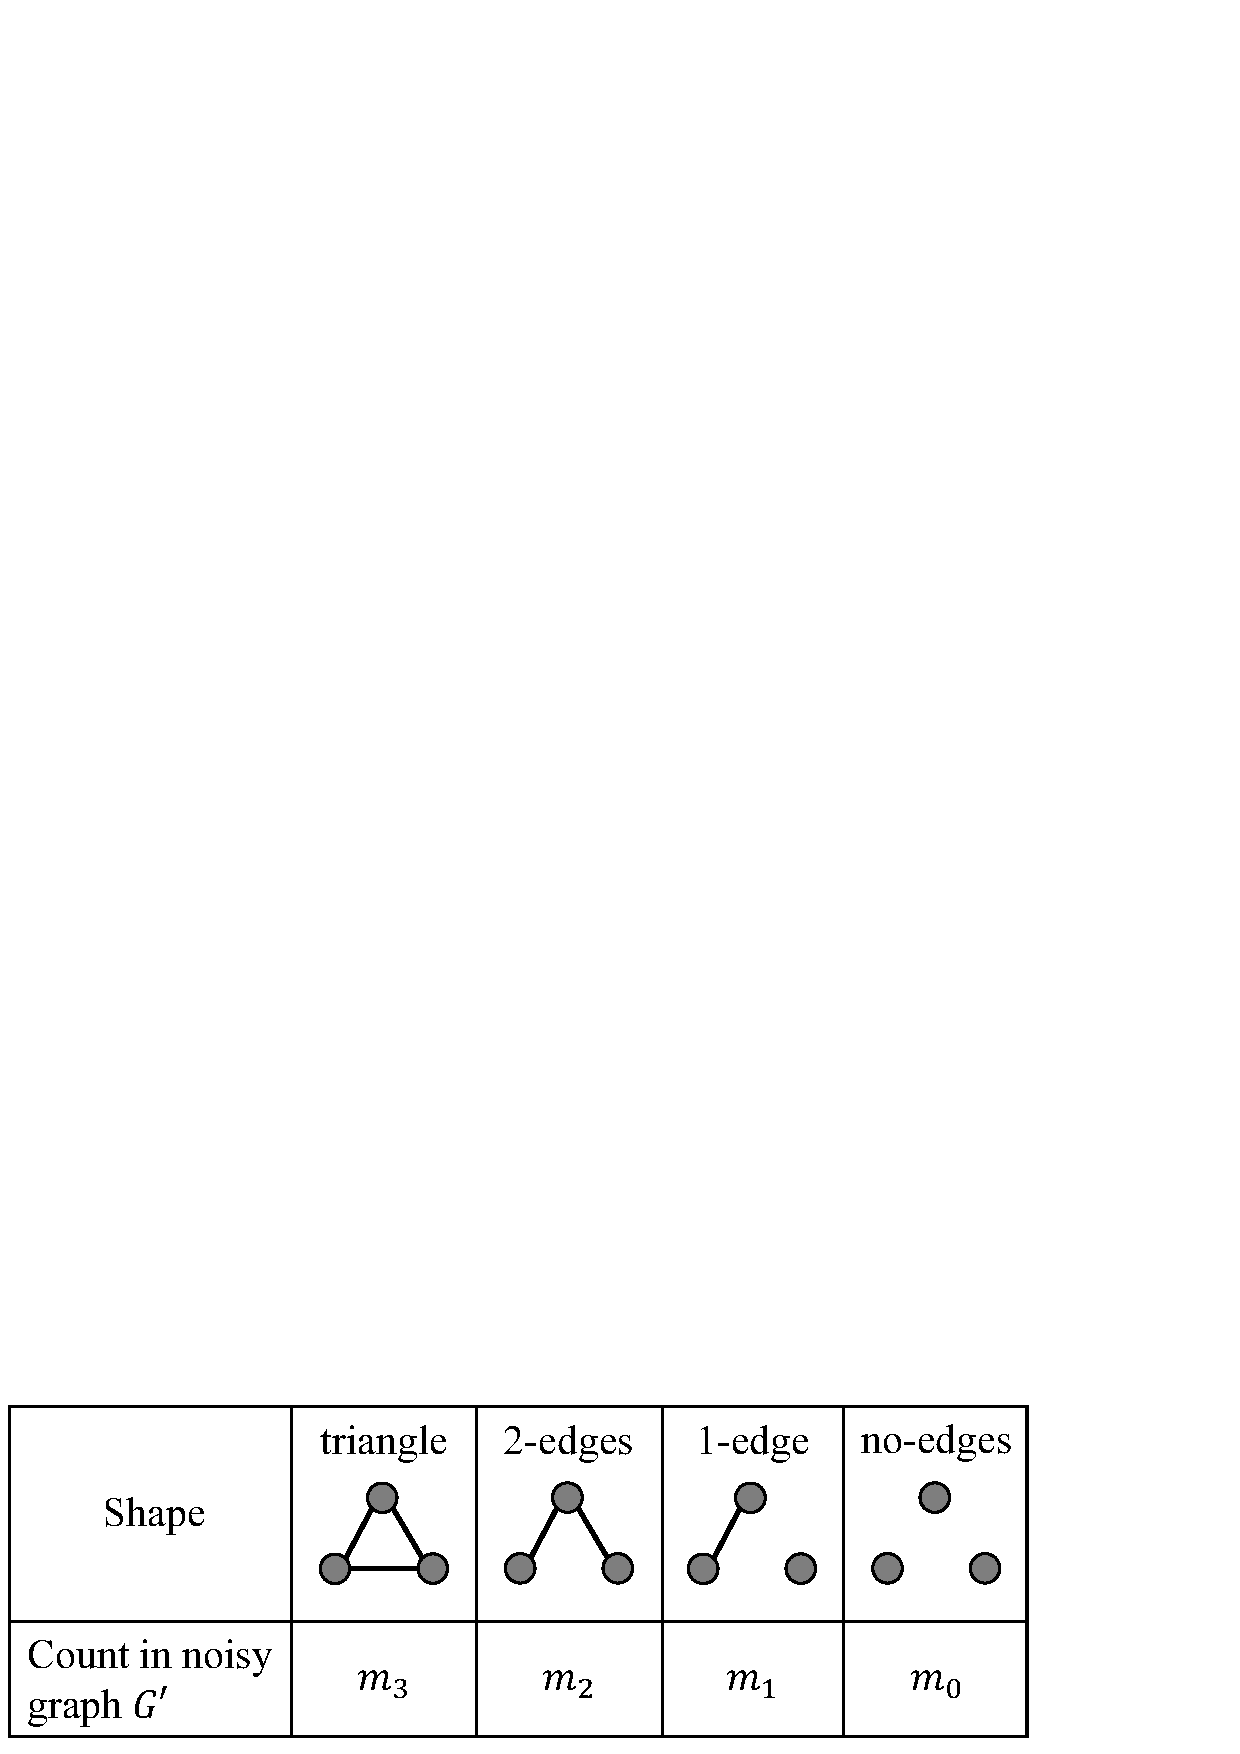
\includegraphics[width=0.9\linewidth]{fig/triplet_shape.pdf}
\caption{Four types of subgraphs with three nodes.}
\label{chap1-fig:triplet_shape}
\end{figure}

Through 
% some 
% a 
clever post-processing 
% method 
known as 
% an 
empirical estimation 
% method~
\cite{Kairouz_ICML16,Murakami_USENIX19,Wang_USENIX17},
we are able to obtain an unbiased estimate of $f_\triangle(G)$ 
% with access to just $P$. 
from $G'$. 
Specifically, a subgraph with three nodes can be divided into four types depending on the number of edges. 
Three nodes with three edges form a triangle. 
We refer to three nodes with two edges, one edge, and no edges as \textit{2-edges},  \textit{1-edge}, and  \textit{no-edges}, respectively. 
Figure~\ref{chap1-fig:triplet_shape} shows their shapes. 
% Let $m_3, m_2, m_1, m_0 \in \nnints$ be respectively the number of triangles, 2-edges, 1-edge, and no-edges in $G'$. 
% Note that $\sum_{i=0}^3 m_i = \binom{n}{3}$. 
% The expectation of 
$f_\triangle(G)$ can be expressed using $m_3$, $m_2$, $m_1$, and $m_0$ as follows:

\begin{proposition}\label{chap1-prop:triangle_emp}
  %Let $\mu = e^\epsilon$. 
  Let $G'=(V,E')$ be a noisy graph generated by applying the RR to the lower triangular part of $\bmA$.
  Let $m_3, m_2, m_1, m_0 \in \nnints$ be respectively the number of triangles, 2-edges, 1-edge, and no-edges in $G'$. 
  Then 
  \begin{align}
      %\textstyle{\mathbb{E}\left[ \frac{\mu^3}{(\mu-1)^3} m_3 - \frac{\mu^2}{(\mu-1)^3} m_2 + \frac{\mu}{(\mu-1)^3} m_1 - \frac{1}{(\mu-1)^3} m_0 \right] = f_\triangle(G).}
      \textstyle{\mathbb{E}\left[ \frac{e^{3\epsilon}}{(e^\epsilon-1)^3} m_3 \hspace{-0.5mm}-\hspace{-0.5mm} \frac{e^{2\epsilon}}{(e^\epsilon-1)^3} m_2 \hspace{-0.5mm}+\hspace{-0.5mm} \frac{e^\epsilon}{(e^\epsilon-1)^3} m_1 \hspace{-0.5mm}-\hspace{-0.5mm} \frac{1}{(e^\epsilon-1)^3} m_0 \right] \hspace{-0.5mm} = \hspace{-0.5mm} f_\triangle(G).}
      \label{chap1-eq:triangle_emp}
  \end{align}
\end{proposition}

% This significantly reduces the $l_2$ error. 
Therefore, the data collector can count $m_3$, $m_2$, $m_1$, and $m_0$ from $G'$, and calculate an unbiased estimate of $f_\triangle(G)$ by (\ref{chap1-eq:triangle_emp}). 
% Algorithm~\ref{chap1-alg:subgraph-rr} contains the precise way to do this.
In Appendix~\ref{chap1-sec:RR_emp}, we show that the $l_2$ loss is significantly reduced by this empirical estimation.

\setlength{\algomargin}{4mm}
\begin{algorithm}
  \SetAlgoLined
  \KwData{Graph $G$ 
  %described by distributed 
  represented as 
  neighbor lists $\bma_1,
    \ldots, \bma_n
  \in \{0,1\}^n$, privacy budget $\epsilon \in \nnreals$.}
  \KwResult{Private estimate of $f_\triangle(G)$.}
  \For{$i=1$ \KwTo $n$}{
    %$R_i \leftarrow (RR_{\epsilon}(a_i^1), \ldots, RR_{\epsilon}(a_i^{i-1}))$\;
    $R_i \leftarrow (RR_{\epsilon}(a_{i,1}), \ldots, RR_{\epsilon}(a_{i,i-1}))$\;
    $release(R_i)$\;
  }
  %$G' \leftarrow \texttt{UndirectedGraph}(R_1, \ldots, R_{i-1})$\;
  $G'=(V,E') \leftarrow \texttt{UndirectedGraph}(R_1, \ldots, R_n)$\;
  %\tcc{Counts $T_3,T_2,T_1,T_0$ in $P$.}
  \tcc{Counts $m_3,m_2,m_1,m_0$ in $G'$.}
  %$\hat{\textbf{m}} \leftarrow \texttt{CountSubgraphs}(G',3)$\;
  $(m_3, m_2, m_1, m_0) \leftarrow \texttt{Count}(G')$\;
  %$\mu \leftarrow e^\epsilon$\;
  %\KwRet{$\frac{1}{(\mu-1)^3}(\mu^3 m_3 -\mu^2 m_2 + \mu m_1 - m_0)$}
  \KwRet{$\frac{1}{(e^\epsilon-1)^3}(e^{3\epsilon} m_3 - e^{2\epsilon} m_2 + e^\epsilon m_1 - m_0)$}

  %\caption{CountSubgraphsRR\label{chap1-alg:subgraph-rr}}
  \caption{\alg{LocalRR$_\triangle$}\label{chap1-alg:subgraph-rr}}
\end{algorithm}

Algorithm~\ref{chap1-alg:subgraph-rr} shows this algorithm. 
In line 2, user $v_i$ applies the RR with privacy budget $\epsilon$ (denoted by $RR_\epsilon$) to $a_{i,1}, \ldots, a_{i,i-1}$ 
% (which corresponds to users $v_1, \ldots, v_{i-1}$ with smaller user IDs) 
in her neighbor list $\bma_i$, and outputs $R_i = (RR_\epsilon(a_{i,1}), \ldots, RR_\epsilon(a_{i,i-1}))$. 
In other words, we apply the RR to the lower triangular part of $\bmA$ and there is no overlap between edges sent by users. 
In line 5, the data collector uses a function (denoted by \texttt{UndirectedGraph}) 
that converts the bits of $(R_1, \ldots, R_n)$ into an undirected graph $G'
= (V, E')$ by adding edge $(v_i,v_j)$ with $i>j$ to $E'$ if and only if the $j$-th bit of
$R_i$ is $1$. 
Note that $G'$ is biased, as explained above. 
In line 6, the data collector uses a function (denoted by 
\texttt{Count}) that calculates $m_3$, $m_2$, $m_1$, and $m_0$ from $G'$. 
Finally, the data collector outputs the expression inside the expectation on
the left-hand side of (\ref{chap1-eq:triangle_emp}), which is an unbiased estimator for 
$f_\triangle(G)$ by Proposition~\ref{chap1-prop:triangle_emp}.
We denote this algorithm by \alg{LocalRR$_\triangle$}.

% One subtlety of Algorithm~\ref{chap1-alg:subgraph-rr} is that, since each edge is known by two users, releasing users' edges through the RR may result in disagreements over the noisy edges. User $i$ may claim that he is
% connected to $j$, and user $j$ may claim he is not connected to $i$. 
% To avoid this problem, we assume an ordering on users, and we let user $i$ ignore edge
% $(i,j)$ if $i<j$. This means each edge is the responsibility of just one user.
% Because edge $(i,j)$ is released by user $\max\{i,j\}$, it is technically a
% directed edge. Thus, we let $P$ be the undirected graph formed by taking the
% direction out of all noisy edges released (Line 5).


\smallskip
\noindent{\textbf{Theoretical properties.}}~~\alg{LocalRR$_\triangle$} 
% Algorithm~\ref{chap1-alg:subgraph-rr} 
provides the following guarantee.

\begin{theorem}\label{chap1-thm:subgraph-rr_LDP}
  \alg{LocalRR$_\triangle$} provides $\epsilon$-edge LDP and $\epsilon$-relationship DP.
\end{theorem}

\alg{LocalRR$_\triangle$} does not have the doubling issue (i.e., it provides not $2\epsilon$ but $\epsilon$-relationship DP), because we apply the RR to the lower triangular part of $\bmA$, as explained in Section~\ref{chap1-sub:LDP}.

Unlike the RR and empirical estimation for tabular data \cite{Kairouz_ICML16}, the expected $l_2$ loss of \alg{LocalRR$_\triangle$} is complicated. 
% due to the fact that multiple triangles can involve the same edge. 
To simplify the utility analysis, we assume that $G$ is generated from the Erd\"os-R\'enyi graph distribution $\bmG(n,\alpha)$ with edge existence probability $\alpha$; i.e., each edge in $G$ with $n$ nodes is independently generated with probability $\alpha \in [0,1]$.
% which generates $G=(V,E)$ with $|V|=n$ with

\begin{theorem}\label{chap1-thm:subgraph-rr}
  Let $\bmG(n,\alpha)$ be the Erd\"os-R\'enyi graph distribution with edge existence probability $\alpha \in [0,1]$. 
  Let $p = \frac{1}{e^\epsilon+1}$ and 
  $\beta = \alpha(1-p) + (1-\alpha)p$. 
  Let 
  %$A(G, \epsilon)$ 
  $\hf_{\triangle}(G, \epsilon)$ 
  be the output of 
  %Algorithm~\ref{chap1-alg:subgraph-rr}.
  \alg{LocalRR$_\triangle$}.
  %Suppose 
  %$G \sim \bmG(n,\frac{d_{max}}{n})$, 
  If 
  $G \sim \bmG(n,\alpha)$, 
  %the Erd\"os-R\'enyi graph
  %distribution with parameter $\frac{d_{max}}{n}$.  Then, 
  then for all 
  $\epsilon \in \nnreals$, 
  %$l_2^2(A(G,\epsilon),
  $\mathbb{E}[l_2^2(\hf_{\triangle}(G, \epsilon),
  f_\triangle(G))] = 
  %O(\frac{e^{6\epsilon}}{(e^\epsilon-1)^6}d_{max}n^3)$.
  O\left(\frac{e^{6\epsilon}}{(e^\epsilon-1)^6}\beta n^4\right)$.
  %Furthermore, Algorithm~\ref{chap1-alg:subgraph-rr} provides $\epsilon$-edge LDP.
\end{theorem}

% Note that Theorem~\ref{chap1-thm:subgraph-rr} is a statement about the expected 
% % average $l_2^2$ error
% $l_2$ loss 
% over graphs 
% % $G \sim \bmG(n,\frac{d_{max}}{n})$. 
% $G \sim \bmG(n,\alpha)$. 
% This is less ideal than the case of
% Theorem~\ref{chap1-thm:k-stars} which upper bounds the 
% % $l_2^2$ error 
% $l_2$ loss for all $G \in \calG$. 
% However, 
% % $\textbf{G}(n,\frac{d_{max}}{n})$ 
% $\textbf{G}(n,\alpha)$ 
% is considered a realistic model from which
% graphs of max degree $d_{max}$ are drawn, so Theorem~\ref{chap1-thm:subgraph-rr} is
% still 
% % a strong bound.
% valid. 

Note that we assume the Erd\"os-R\'enyi model only for the utility analysis of \alg{LocalRR$_\triangle$}, and do not assume this model for the other algorithms. 
The upper-bound of \alg{LocalRR$_\triangle$} in Theorem~\ref{chap1-thm:subgraph-rr} is less ideal than the upper-bounds of the other algorithms in that it does not consider all possible graphs $G \in \calG$. 
Nevertheless, we also show that the $l_2$ loss of \alg{LocalRR$_\triangle$} is roughly consistent with Theorem~\ref{chap1-thm:subgraph-rr} in our experiments using two real datasets (Section~\ref{chap1-sec:experiments}) and 
% artificial graphs based on 
the Barab\'{a}si-Albert graphs \cite{NetworkScience}, which have power-law degree distribution (Appendix~\ref{chap1-sec:BAGraph}). 

% The parameter $\alpha$ is very small in a sparse graph. 
% For example, it is reasonable to assume that $\alpha \leq \frac{d_{max}}{n} \ll 1$. 
% On the other hand, $\beta$ is a parameter in 
The parameters $\alpha$ and $\beta$ are edge existence probabilities in the original graph $G$ and noisy graph $G'$, respectively. 
Although $\alpha$ is very small in a sparse graph, $\beta$ can be large for small $\epsilon$. 
For example, if $\alpha \approx 0$ and $\epsilon=1$, then $\beta \approx \frac{1}{e+1} = 0.27$. 
% In this case, the expected $l_2$ loss of \alg{LocalRR$_\triangle$} can be expressed as: $O\left(\frac{e^{6\epsilon}}{(e^\epsilon-1)^6}d_{max} n^3\right)$.

Theorem~\ref{chap1-thm:subgraph-rr} states that for large $n$, the $l_2$ loss of \alg{LocalRR$_\triangle$} 
($=O(n^4)$) 
% ($=O(d_{max}n^3)$) 
is much larger than the $l_2$ loss of \alg{LocalRR$_k\star$} ($=O(n)$). 
This follows from the fact that user $v_i$ 
% cannot see any edge $(v_j, v_k) \in E$ in graph $G$ and 
is not aware of any triangle formed by $(v_i, v_j, v_k)$, as explained above. 

In contrast, counting $f_\triangle(G)$ in the centralized model is much easier because the data collector sees all triangles in $G$; i.e., the data collector knows $f_\triangle(G)$. 
% After we perform graph projection 
% \cite{Day_SIGMOD16,Kasiviswanathan_TCC13,Raskhodnikova_arXiv15} 
% so that each user's degree does not exceed $\td_{max}$, 
% the 
The 
% local 
% global 
sensitivity of $f_\triangle$ 
% becomes 
is 
at most $\td_{max}$ (after graph projection). 
% Therefore, as with $k$-stars, 
Thus, 
we can consider a simple algorithm that 
% performs graph projection so that each user's degree never exceeds $\td_{max}$, 
% and then 
% adds the Laplacian noise $\Lap(\td_{max}/\epsilon)$ 
% ($\td_{max} > d_{max}$) 
% to $f_{\triangle}(G)$, and 
outputs $f_{\triangle}(G) + \Lap(\td_{max}/\epsilon)$. 
We denote this algorithm by \alg{CentralLap$_{\triangle}$}. 
\alg{CentralLap$_{\triangle}$} attains the expected $l_2$ loss ($=$ variance) of $O\left(\frac{\td_{max}^2}{\epsilon^2}\right)$. 

% \colorB{In Section~\ref{chap1-sub:two_rounds}, we propose a two-rounds LDP algorithm for triangles to significantly reduce the $l_2$ loss in the local model.}

% In Algorithm~\ref{chap1-alg:subgraph-rr}, 
The large $l_2$ loss of \alg{LocalRR$_\triangle$} is caused by the fact that 
each edge is released independently with
some probability of being flipped. 
% Thus, 
In other words, 
there are three independent random
variables that influence 
% any subgraph of size $3$ in $P$. 
any triangle in $G'$. 
The next algorithm,
using interaction, 
% is able to reduce 
reduces 
this influencing number 
% to two, 
from three to one 
% because 
% a single 
by using the fact that 
a user 
% always 
knows 
% two edges of a subgraph of size 3.
the existence of two edges for any triangle that involves the user. 

% \ji{Can we combine the last and third-last paragraphs of this section?}
% \tm{It's a little bit difficult to me because 
% the explanation is in the order of ``Thm 4 --> one-round local (third-last) --> centralized (second-last) --> two-round local (last) (--> Sec 4.3)''. Instead, I shortened the third-last paragraph.}

% \subsection{Two-Rounds LDP Algorithms for Triangles}
\subsection{Two-Rounds Algorithms for Triangles}
% \colorB{Sequentially Interactive Graph LDP Algorithms}}
\label{chap1-sub:two_rounds}

\noindent{\textbf{Algorithm.}}~~Allowing for 
% sequential interaction, 
two-rounds interaction, 
we are able to compute $f_{\triangle}$ with
a significantly improved $l_2$ loss, albeit with a higher per-user
communication overhead.
As described in Section~\ref{chap1-sub:non-interactive_triangles}, it is impossible for user $v_i$ to see edge $(v_j, v_k) \in E$ in graph $G=(V,E)$ at the first round. 
However, if 
% each user $v_i$ applies the RR to her neighbor list $\bma_i$ as in \alg{LocalRR$_\triangle$} and 
the data collector publishes a noisy graph $G'=(V,E')$ calculated by \alg{LocalRR$_\triangle$} at the first round, then 
user $v_i$ can see a noisy edge $(v_j, v_k) \in E'$ in the noisy graph $G'$ at the second round. 
Then user $v_i$ can count the number of \textit{noisy triangles} formed by
$(v_i, v_j, v_k)$ such that $(v_i,v_j) \in E$, $(v_i,v_k) \in E$, and $(v_j,v_k)
\in E'$, and send the noisy triangle counts with the Laplacian noise to the data
collector in an analogous way to \alg{LocalLap$_{k\star}$}.
Since user $v_i$ always knows that two edges $(v_i,v_j)$ and $(v_i,v_k)$ exist in $G$, 
there is only one noisy edge in any noisy triangle 
(whereas all edges are noisy in \alg{LocalRR$_\triangle$}).
% edge $(v_j,v_k)$
% random variable 
% that influences the existence of the triangle $(v_i, v_j, v_k)$ in $G$. 
This is an intuition behind our proposed two-rounds algorithm. 

As with the RR in Section~\ref{chap1-sub:non-interactive_triangles}, simply counting the noisy triangles can introduce a bias. 
Therefore, we calculate an empirical estimate of $f_\triangle(G)$ from the noisy triangle counts. 
Specifically, 
% we calculate the expectation of 
the following is the empirical estimate of $f_\triangle(G)$: 
% can be expressed as follows:
% Specifically, assume that the data collector publishes a noisy graph $G'=(V,E')$ calculated by \alg{LocalRR$_\triangle$} with privacy budget $\epsilon_0 \in \nnreals$ at the first round. 
% Let $t_i \in \nnints$ be the number of triplets $(v_i, v_j, v_k)$ such that $j < i < k$, $(v_i,v_j) \in E$, $(v_i,v_k) \in E$, and $(v_j,v_k) \in E'$; i.e., 
% the number of noisy triangles user $v_i$ can see at the second round. 
% Here we count only triplets $(v_i, v_j, v_k)$ with $j < i < k$ to avoid counting the same triplet multiple times.
% Let $s_i \in \nnints$ be the number of triplets $(v_i, v_j, v_k)$ such that $j < i < k$, $(v_i,v_j) \in E$, and $(v_i,v_k) \in E$; i.e., 
% the number of $2$-stars of which user $v_i$ is a center. 
% Then the expectation of $f_\triangle(G)$ can be calculated from $\epsilon_0$, $t_i$, and $s_i$ as follows:

\begin{proposition}\label{chap1-prop:triangle_emp_2rounds}
  Let $G'=(V,E')$ be a noisy graph generated by applying the RR with privacy budget $\epsilon_1 \in \nnreals$   to the lower triangular part of $\bmA$.
  Let $p_1 = \frac{1}{e^{\epsilon_1}+1}$. 
  Let $t_i \in \nnints$ be the number of triplets $(v_i, v_j, v_k)$ such that 
  %$j < i < k$, 
  $j < k < i$, 
  $(v_i,v_j) \in E$, $(v_i,v_k) \in E$, and $(v_j,v_k) \in E'$.
  Let $s_i \in \nnints$ be the number of triplets $(v_i, v_j, v_k)$ such that 
  %$j < i < k$, 
  $j < k < i$, 
  $(v_i,v_j) \in E$, and $(v_i,v_k) \in E$. 
  Let $w_i = t_i - p_1 s _i$. 
  Then 
  \begin{align}
      %\textstyle{\mathbb{E}[f_\triangle(G)] = \frac{1}{1-2p_1} \sum_{i=1}^n (t_i - p_1 s_i)}.
      \textstyle{\mathbb{E}\left[ \frac{1}{1-2p_1} \sum_{i=1}^n w_i \right] = f_\triangle(G).}
      \label{chap1-eq:triangle_emp_2rounds}
  \end{align}
\end{proposition}

Note that in Proposition~\ref{chap1-prop:triangle_emp_2rounds}, 
we count only triplets $(v_i, v_j, v_k)$ with 
% $j < i < k$ 
$j < k < i$ 
% to avoid counting the same triplet multiple times. 
to use only the lower triangular part of $\bmA$. 
$t_i$ is the number of noisy triangles user $v_i$ can see at the second round. 
$s_i$ is the number of $2$-stars of which user $v_i$ is a center. 
Since $t_i$ and $s_i$ can reveal information about an edge in $G$, user $v_i$ adds the Laplacian noise to $w_i$ $(= t_i - p_1 s _i)$ in (\ref{chap1-eq:triangle_emp_2rounds}), and sends it to the data collector. 
Then the data collector calculates an unbiased estimate of $f_\triangle(G)$ by (\ref{chap1-eq:triangle_emp_2rounds}). 

% Instead of releasing each edge through 
% randomized
% response, user $i$ is given a specific query depending on $P_{i-1}$, the
% subgraph of $G$ on users $1$ through $i-1$ released through randomized response.
% Like Algorithm~\ref{chap1-alg:subgraph-rr}, we assume user $i$ ignores edge $(i,j)$ if
% $i<j$. The query to user $i$ is to noisily count the number of triangles of which he is
% a part, using two of his edges and one edge in $P_{i-1}$. He releases this
% number and a randomized response on his edges so that future users may build
% $P_{i}$. 

\setlength{\algomargin}{5mm}
\begin{algorithm}
  \SetAlgoLined
  \KwData{Graph $G$ 
  %described by distributed 
  represented as 
  neighbor lists $\bma_1,
    \ldots, \bma_n
    \in \{0,1\}^n$, two privacy budgets
  %$\epsilon_0,\epsilon_1 > 0$.}
  $\epsilon_1,\epsilon_2 > 0$, $\td_{max} \in \nnints$.}
  %\KwResult{Private count of number of triangles in $G$.}
  \KwResult{Private estimate of $f_\triangle(G)$.}
  %$\rho \leftarrow \frac{1}{e^{\epsilon_0}+1}$\;
  $p_1 \leftarrow \frac{1}{e^{\epsilon_1}+1}$\;
  \tcc{First round.}
  \For{$i=1$ \KwTo $n$}{
    %$ans_i \leftarrow 0$\;
    %$R_i \leftarrow (RR_{\epsilon_0}(a_i^1), \ldots, RR_{\epsilon_0}(a_i^{i-1}))$\;
    $R_i \leftarrow (RR_{\epsilon_1}(a_{i,1}), \ldots, RR_{\epsilon_1}(a_{i,i-1}))$\;
    $release(R_i)$\;
  }
  %$P_{i-1} \leftarrow \texttt{UndirectedGraph}(R_1, \ldots, R_{i-1})$\;
  $G'=(V,E') \leftarrow \texttt{UndirectedGraph}(R_1, \ldots, R_{i-1})$\;
  \tcc{Second round.}
  \For{$i=1$ \KwTo $n$}{
    $\bma_i \leftarrow \texttt{GraphProjection}(\bma_i, \td_{max})$\;
    %$t_i \leftarrow |\{(u,v) : u,v \in [i], u<v<i, a_{i}^u = a_{i}^v = 1,(u,v) \in P_{i-1}\}|$\;
    $t_i \leftarrow |\{(v_i,v_j,v_k) : 
    %j<i<k, a_{j,i} = a_{i,k} = 1, 
    j<k<i, a_{i,j} = a_{i,k} = 1, 
    (v_j,v_k) \in E'\}|$\;
    %$s_i \leftarrow |\{(u,v) : u,v \in [i], u<v<i, a_{i}^u = a_{i}^v = 1\}|$\;
    $s_i \leftarrow |\{(v_i,v_j,v_k) : 
    %j<i<k, a_{j,i} = a_{i,k} = 1\}|$\;
    j<k<i, a_{i,j} = a_{i,k} = 1\}|$\;
    %$w_i \leftarrow t_i - \rho s_i + Lap(\frac{d_{max}(1-\rho)}{\epsilon_1})$\;
    %$w_i \leftarrow t_i - p_1 s_i + \Lap(\frac{\td_{max}(1-p_1)}{\epsilon_2})$\;
    $w_i \leftarrow t_i - p_1 s_i$\;
    $\hw_i \leftarrow w_i + \Lap(\frac{\td_{max}}{\epsilon_2})$\;
    %$release(R_i, w_i)$\;
    $release(\hw_i)$\;
  }
  %$ans \leftarrow \frac{1}{1-2\rho}\sum_{i=1}^n w_i$\;
  \KwRet{$\frac{1}{1-2p_1}\sum_{i=1}^n \hw_i$}
  %\caption{CountSubgraphsTwoRound\label{chap1-alg:subgraph-interactive}}
  \caption{\alg{Local2Rounds$_\triangle$}}\label{chap1-alg:subgraph-interactive}
\end{algorithm}

Algorithm~\ref{chap1-alg:subgraph-interactive} contains the formal
description of this process. 
It takes as input a graph $G$, 
% (represented as neighbor lists $\bma_1, \ldots, \bma_n$), 
the privacy budgets $\epsilon_1, \epsilon_2 \in \nnreals$ at the first and second rounds, respectively, 
and 
% It also takes as input 
% an upper-bound $\td_{max}$ on the maximum degree $d_{max}$ of $G$ 
a non-negative integer $\td_{max} \in \nnints$. 
% in the same way as \alg{LocalLap$_{k\star}$}. 
% We will describe the private computation of $d_{max}$ with edge LDP at the end of Section~\ref{chap1-sub:two_rounds}. 
At the first round, we 
apply the RR to the lower triangular part of $\bmA$ 
(i.e., there is no overlap between edges sent by users) 
% . 
and use the \texttt{UndirectedGraph} function to 
obtain a noisy graph $G'=(V,E')$ by the RR in the same way as Algorithm~\ref{chap1-alg:subgraph-rr}. 
Note that $G'$ is biased. 
We calculate an unbiased estimate of $f_\triangle(G)$ from $G'$ at the second round.  
% Then we use the \texttt{UndirectedGraph} function, which makes an undirected graph $G'
% = (V, E')$ by adding edge $(i,j)$ with $i>j$ to $E'$ if and only if the $j$-th bit of $R_i$ is $1$. 

At the second round, each user $v_i$ 
calculates $\hw_i = w_i + \Lap(\frac{\td_{max}}{\epsilon_2})$ 
%  and 
by adding the Laplacian noise to $w_i$ 
% $(= t_i - p_1 s _i)$, 
in Proposition~\ref{chap1-prop:triangle_emp_2rounds} 
whose 
% local 
% global 
sensitivity is at most 
% $d_{max} (1-p_1)$, 
$\td_{max}$ 
% (after graph projection), 
(as we will prove in Theorem~\ref{chap1-thm:local2rounds_LDP}). 
Finally, we output $\frac{1}{1-2p_1}\sum_{i=1}^n \hw_i$, which is an unbiased estimate of $f_\triangle(G)$ by Proposition~\ref{chap1-prop:triangle_emp_2rounds}. 
We call this algorithm \alg{Local2Rounds$_\triangle$}.

% The intuitive reason Algorihtm~\ref{chap1-alg:subgraph-interactive} performs better than 
% Algorithm~\ref{chap1-alg:subgraph-rr} is that a noisy triangle is counted using two 
% noisy computations, the noisy edge in
% $P_{i-1}$ and user $i$'s noisy count. In Algorithm~\ref{chap1-alg:subgraph-rr}, each
% subgraph of size $3$ in $P$ is the result of three noisy computations.

\smallskip
\noindent{\textbf{Theoretical properties.}}~~\alg{Local2Rounds$_\triangle$} 
% Algorithm~\ref{chap1-alg:subgraph-interactive} 
has the following 
% performance 
guarantee.

\begin{theorem}\label{chap1-thm:local2rounds_LDP}
  %If the maximum degree $d_{max}$ of $G$ is at most $\td_{max}$, 
  \alg{Local2Rounds$_\triangle$}
  provides $(\epsilon_1 + \epsilon_2)$-edge LDP and $(\epsilon_1 + \epsilon_2)$-relationship DP.
\end{theorem}

As with \alg{LocalRR$_\triangle$}, \alg{Local2Rounds$_\triangle$} does not have the doubling issue; i.e., it provides $\epsilon$-relationship DP (not $2\epsilon$). 
This follows from the fact that we 
use only the lower triangular part of $\bmA$; 
% count each triplet $(v_i,v_j,v_k)$ only once; 
i.e., we assume 
%$j<i<k$ 
$j<k<i$ 
in counting $t_i$ and $s_i$. 

\begin{theorem}\label{chap1-thm:local2rounds}
  Let 
  %$A(G, d_{max}, \epsilon_0, \epsilon_1)$ 
  $\hf_{\triangle}(G, \epsilon_1, \epsilon_2, \td_{max})$ 
  be the output of 
  %Algorithm~\ref{chap1-alg:subgraph-interactive}. 
%   \alg{LocalRR$_\triangle$}. 
  \alg{Local2Rounds$_\triangle$}. 
  Then, for all 
  %$d_{max} \in \nats$,
  $\epsilon_1,\epsilon_2 \in \nnreals$, 
  $\td_{max} \in \nnints$,
  and $G\in \calG$ such that the
  maximum degree $d_{max}$ of $G$ is 
  at most 
  $\td_{max}$,
  %$l_2^2(A(G,d_{max},\epsilon_0,\epsilon_1) 
  $\mathbb{E}[l_2^2(\hf_{\triangle}(G, \epsilon_1, \epsilon_2, \td_{max}), f_\triangle(G))] 
  \leq
    O\left(\frac{e^{\epsilon_1}}{(1-e^{\epsilon_1})^2} \left(\td_{max}^3 n +
    \frac{e^{\epsilon_1}}{\epsilon_2^2}\td_{max}^2 n\right)\right)$.
\end{theorem}

Theorem~\ref{chap1-thm:local2rounds} means that for triangles, the $l_2$ loss 
% of \alg{LocalRR_$\triangle$} 
is reduced from $O(n^4)$ to $O(\td_{max}^3n)$ by introducing an additional round. 

% The upper and lower bounds on the $l_2$ losses for the central,
% % local non-interactive, 
% one-round local, 
% and 
% % local sequentially interactive 
% two-rounds local 
% models discussed in
% this section appear in Table~\ref{chap1-tab:perf}.

\smallskip
\noindent{\textbf{Private calculation of $d_{max}$.}}~~As with $k$-stars, we can privately calculate $d_{max}$ 
% with edge LDP 
by using the method described in Section~\ref{chap1-sub:non-interactive_k_stars}. 
Furthermore, the private calculation of $d_{max}$ does not increase the number of rounds; i.e., we can run \alg{Local2Rounds$_\triangle$} with the private calculation of $d_{max}$ in two rounds. 

Specifically, let $\epsilon_0 \in \nnreals$ be the privacy budget for the private calculation of $d_{max}$. 
At the first round, each user $v_i$ adds $\Lap(\frac{1}{\epsilon_0})$ to her degree $d_i$, 
% (i.e., number of ``$1$''s in her neighbor list $\bma_i$), 
and sends the noisy degree $\hd_i$ ($=d_i + \Lap(\frac{1}{\epsilon_0})$) to the data collector, along with the outputs $R_i = (RR_\epsilon(a_{i,1}), \ldots, RR_\epsilon(a_{i,i-1}))$ of the RR. 
The data collector calculates the noisy max degree $\hd_{max}$ ($= \max\{\hd_1,
\ldots, \hd_n\}$) as an estimate of $d_{max}$, and sends it back to all users. 
At the second round, we run \alg{Local2Rounds$_\triangle$} with input $G$ (represented as $\bma_1, \ldots, \bma_n$), $\epsilon_1$, $\epsilon_2$, and $\lfloor \hd_{max} \rfloor$. 

% At the second round, each user performs graph projection; i.e., if $d_i$ exceeds $\hd_{max}$, user $v_i$ randomly selects $\hd_{max}$ neighbors from her neighbor list $\bma_i$ (otherwise, user $v_i$ uses $\bma_i$ as it is). 
% Let $\bma'_i \in \{0,1\}^n$ be a neighbor list of user $v_i$ after this projection. 
% We run the second round part (lines $7$ to $12$) of \alg{Local2Rounds$_\triangle$} with input $\bma'_1, \ldots, \bma'_n$, $\epsilon_1$, $\epsilon_2$, 
% and $\hd_{max}$. 

At the first round, the calculation of $\hd_{max}$ provides $\epsilon_0$-edge LDP. 
% because each user's degree has the sensitivity $1$ under edge LDP. 
Note that it provides $2\epsilon_0$-relationship DP (i.e., it has the doubling issue) because one edge $(v_i,v_j) \in E$ affects both of the degrees $d_i$ and $d_j$ by 1. 
At the second round, \alg{LocalLap$_{k\star}$} provides $(\epsilon_1 + \epsilon_2)$-edge LDP and 
$(\epsilon_1 + \epsilon_2)$-relationship DP (Theorem~\ref{chap1-thm:local2rounds_LDP}). 
% because each user $v_i$'s degree in $\bma'_i$ never exceeds $\hd_{max}$. 
% (and then Theorem~\ref{chap1-thm:local2rounds_LDP} holds). 
Then by the composition theorem~\cite{DP}, this two-rounds algorithm provides $(\epsilon_0 + \epsilon_1 + \epsilon_2)$-edge LDP and $(2\epsilon_0 + \epsilon_1 + \epsilon_2)$-relationship DP. 
Although the total privacy budget is larger for relationship DP, the difference ($=\epsilon_0$) can be very small. 
In fact, we set $(\epsilon_0, \epsilon_1, \epsilon_2) = (0.1, 0.45, 0.45)$ or $(0.2, 0.9, 0.9)$ in our experiments (i.e., the difference is $0.1$ or $0.2$), and show that this algorithm provides almost the same utility as \alg{Local2Rounds$_\triangle$} with the true max degree $d_{max}$. 

\smallskip
\noindent{\textbf{Time complexity.}}~~We also note that \alg{Local2Rounds$_\triangle$} has an advantage over \alg{LocalRR$_\triangle$} in terms of the time complexity. 
% in addition to the expected $l_2$ loss. 

Specifically, \alg{LocalRR$_\triangle$} is inefficient because the data collector has to count the number of triangles $m_3$ in the noisy graph $G'$. 
Since the noisy graph $G'$ is dense (especially when $\epsilon$ is small) and there are $\binom{n}{3}$ subgraphs with three nodes in $G'$, the number of triangles is $m_3 = O(n^3)$. 
Then, the time complexity of \alg{LocalRR$_\triangle$} is 
% $O(n)$ for each user's part and $O(n^3)$ for the data collector's part, 
also $O(n^3)$, which is not practical for a graph with a large number of users $n$.
In fact, we implemented \alg{LocalRR$_\triangle$} ($\epsilon=1$) with C/C++ and measured its running time using one node of a supercomputer (ABCI: AI Bridging Cloud Infrastructure \cite{ABCI}). 
When $n=5000$, $10000$, $20000$, and $40000$, the running time was $138$, $1107$, $9345$, and $99561$ seconds, respectively; i.e., the running time was almost cubic in $n$. 
We can also estimate the running time for larger $n$. 
For example, when $n=1000000$, \alg{LocalRR$_\triangle$} ($\epsilon=1$) would require about $35$ years $(=1107 \times 100^3 /(3600 \times 24 \times 365))$. 
% Even if we use $1000$ nodes of the supercomputer (the ABCI has $1088$ nodes \cite{ABCI}) in parallel, \alg{LocalRR$_\triangle$} would require over $10$ days. 

In contrast, the time complexity of \alg{Local2Rounds$_\triangle$} 
% for each user 
is 
% $O(n)$ in the first round (l.3-4 in Algorithm~\ref{chap1-alg:subgraph-interactive}) and $O(d_{max}^2)$ in the second round (l.8-13 in Algorithm~\ref{chap1-alg:subgraph-interactive})). 
% $O(n + d_{max}^2)$ for each user's part and $O(n)$ for the data collector's part at the second round. 
$O(n^2 + n d_{max}^2)$\footnote{When we 
% want to 
evaluate 
% the utility of 
\alg{Local2Rounds$_\triangle$} in our experiments, 
% When we evaluate the utility of \alg{Local2Rounds$_\triangle$} on one computer, 
we can apply the RR to only edges that are required at the second round; i.e., $(v_j,v_k) \in G'$ in line 8 of Algorithm~\ref{chap1-alg:subgraph-interactive}. 
Then the time complexity of \alg{Local2Rounds$_\triangle$} 
% is 
can be reduced to 
$O(n d_{max}^2)$ in total. 
We also confirmed that when $n=1000000$, the running time of \alg{Local2Rounds$_\triangle$} was $311$ seconds on one node of the ABCI. 
% , which is $3.5 \times 10^6$ times faster than \alg{LocalRR$_\triangle$}. 
Note, however, that this does \textit{not} protect individual privacy, because it reveals the fact that users $v_j$ and $v_k$ are friends with $u_i$ to the data collector.}. 
% including the private calculation of $d_{max}$. 
The factor of $n^2$ comes from the fact that the size of the noisy graph $G'$ is $O(n^2)$. 
This also causes a large communication overhead, as explained below.
% Further reduction of the time complexity by compressing the graph size (e.g., via graph projection) is left for future work.}

\smallskip
\noindent{\textbf{Communication overhead.}}~~In 
% The \alg{Local2Rounds$_\triangle$} has a quadratic communication overhead.
\alg{Local2Rounds$_\triangle$}, each user need to see the noisy graph $G'$ 
of size $O(n^2)$ 
% with $O(n^2)$ bits 
to count $t_i$ and $s_i$. 
% must count $t_i$ and $s_i$ which depend on $G'$, the private graph computed in the first round. 
% Thus, each user must see $G'$, a graph with $O(n^2)$ bits. 
This results in a per-user communication overhead of $O(n^2)$. 
% We 
Although we 
do not simulate the communication overhead in our experiments that use \alg{Local2Rounds$_\triangle$}, 
% but 
the $O(n^2)$ overhead 
% would 
might 
limit its application in very large graphs. 
An interesting avenue of future work is how to compress the graph size (e.g., via graph projection or random projection) to reduce both the time complexity and the communication overhead.
% Again, compressing the graph size (e.g., via graph projection) is left for future work.

\begin{table*}
  \centering
\begin{tabular}{|l|l|p{3.5cm}|p{3cm}|l|l|l|}
  \hline
  & Centralized & \spantwo{One-round local} & Two-rounds local \\
  \hline
  & Upper Bound & Lower Bound & Upper Bound & Upper Bound \\ \hline

  $f_{k\star}$
  & $O\left( \frac{d_{max}^{2k-2}}{\epsilon^2} \right)$  
  &  $\Omega\left( \frac{e^{2\epsilon}}{(e^{2\epsilon}+1)^2}d_{max}^{2k-2}n \right)$ 
  &  $O\left( \frac{d_{max}^{2k-2}}{\epsilon^2}n \right)$ 
  &  $O\left( \frac{d_{max}^{2k-2}}{\epsilon^2}n \right)$ \\ \hline

 $f_\triangle$ 
  &  $O\left(\frac{d_{max}^2}{\epsilon^2}\right)$ 
  &  $\Omega\left( \frac{e^{2\epsilon}}{(e^{2\epsilon}+1)^2}d_{max}^2n \right)$
  &  $O\left(\frac{e^{6\epsilon}}{(e^{\epsilon}-1)^6}n^4\right)$ 
  (when $G \sim \bmG(n,\alpha)$)
  %(randomized bound)
  &  $O\left(\frac{e^\epsilon}{(e^\epsilon-1)^2}(d_{max}^3 n +
  \frac{e^\epsilon}{\epsilon^2}d_{max}^2 n)\right)$ \\ \hline

\end{tabular}
\caption{Bounds on $l_2$ losses for privately estimating $f_{k\star}$ and
$f_{\triangle}$ with $\epsilon$-edge LDP. For upper-bounds, we assume that  $\td_{max}=d_{max}$. 
For the centralized model, we use the Laplace mechanism. For
the one-round $f_\triangle$ algorithm, we apply Theorem~\ref{chap1-thm:subgraph-rr} 
with constant $\alpha$. For the two-round protocol $f_\triangle$ algorithm, we
apply Theorem~\ref{chap1-thm:local2rounds} with
$\epsilon_1=\epsilon_2=\frac{\epsilon}{2}$. }\label{chap1-tab:perf}
\end{table*}

\subsection{Lower Bounds}
\label{chap1-sub:lower_bounds}

We show a general lower bound on the $l_2$ loss of private estimators $\hat{f}$ of
real-valued functions $f$ in the one-round LDP model. Treating $\epsilon$ as a
constant, we have shown that 
when $\td_{max}=d_{max}$, 
% for graphs $G$ of maximum degree $d_{max}$,
the expected $l_2$ loss of \alg{LocalLaplace$_{k\star}$} is 
% $l_2^2(\alg{LocalLaplace$_{k\star}$}(G), f_{k\star}(G)) = 
$O(nd_{max}^{2k-2})$
(Theorem~\ref{chap1-thm:k-stars}). 
% and 
% the expected $l_2$ loss of 
% \alg{Local2Rounds$_\triangle$} is 
% \alg{LocalRR$_\triangle$} is 
%$l_2^2(\alg{LocalRR$_\triangle$}(G),
% f_{k\star}(G) ) = 
% $O(nd_{max}^2)$ 
% $O(nd_{max}^3)$ 
% $O(n^4)$ 
% (Theorem~\ref{chap1-thm:local2rounds}). 
% (Theorem~\ref{chap1-thm:subgraph-rr}). 
However, in
the centralized 
% edge-DP 
model, we can use
the Laplace mechanism with sensitivity 
$2\binom{d_{max}}{k-1}$ 
% and 
%$d_{max}^2$,
% $d_{max}$ 
% respectively, 
to obtain $l_2^2$ errors of $O(d_{max}^{2k-2})$ 
% and
% $O(d_{max}^2)$, respectively 
for $f_{k\star}$. 
% and $f_\triangle$. 
Thus, we ask
if 
% the factors of $n$ are 
the factor of $n$ is 
necessary 
% in the local model. 
in the one-round LDP model.

We 
% partially 
answer this question affirmatively.
We show for many types of queries $f$, there is a lower bound on 
% $l_2^2(f(\bmA), \hf(\bmA))$ 
$l_2^2(f(G), \hf(G))$ 
for any private estimator $\hf$ of the form
\begin{equation}\label{chap1-eq:one-round-lower}
%   \hf(\bmA) = \tilde{f}(\calR_1(\bma_1), \ldots, \calR_n(\bma_n)).
  \hf(G) = \tilde{f}(\calR_1(\bma_1), \ldots, \calR_n(\bma_n)),
\end{equation}
where 
$\calR_1, \ldots, \calR_n$ satisfy 
% $\epsilon$-relationship or $\epsilon$-edge DP 
$\epsilon$-edge LDP or $\epsilon$-relationship DP 
and $\tilde{f}$ is an aggregate function that takes $\calR_1(\bma_1), \ldots, \calR_n(\bma_n)$ as input and outputs $\hf(G)$. 
Here we assume that $\calR_1, \ldots, \calR_n$ 
% and 
are independently run, meaning that they are in the one-round
setting.
% 
% Our lower bound has the form of $\Omega(nD^2)$, where $D$ is a positive real
% number depending on $f$ that is similar to, but stronger than, the global sensitivity $GS_f$.
% Global sensitivity by itself cannot provide a strong lower bound in the
% local model. As a counterexample, if $f$ were the function that is always $0$ or $GS_f$,
% then an estimator $\hf$ that predicts $0$ would satisfy
% $l_2^2(f(\bmA),\hf(\bmA)) = O(GS_f^2)$
% for all adjacency matrices $\bmA$. 
% 
% Instead, we 
For our 
%this 
lower bound,
% we consider $f$ to be a function on graphs. 
% not matrices. 
% Then 
% We 
we 
require 
that 
input edges to $f$ 
% to 
be ``independent'' in the sense that 
% and 
adding an edge to an input graph $G$  
independently 
% increase 
change 
$f$ by at least $D \in \reals$. 
% over a set of input graphs. 
% Notice that we consider $f$ to be a function on graphs, not
% matrices, for this lower bound. 
The specific structure of input graphs we require is as follows:

\begin{definition}\label{chap1-def:mono-cube}[$(n,D)$-independent cube for $f$]
  Let 
  %$D \in \reals$. 
  $D \in \nnreals$. 
  For 
  %$k \in \nats$, 
  $\kappa \in \nats$, 
  let $G=(V,E) \in \calG$ be a graph on 
  %$n = 2k$ 
  $n = 2\kappa$ 
  nodes, and let 
  %$M = \{(v_{i_1}, v_{i_2}),(v_{i_3},v_{i_4}),\ldots,(v_{i_{2k-1}},v_{i_{2k}})\}$ 
  $M = \{(v_{i_1}, v_{i_2}),(v_{i_3},v_{i_4}),\ldots,(v_{i_{2k-1}},v_{i_{2\kappa}})\}$ 
  for integers $i_j \in [n]$ 
  %denote 
  be 
  a set of edges such that each of $i_1, \ldots, i_{2\kappa}$ is distinct (i.e., perfect matching on the nodes).
%   a perfect
%   matching on the 
%   nodes, 
%   meaning each 
%   of $i_1, \ldots, i_{2k}$ 
%   is distinct. 
  %Furthermore,
  Suppose that 
  %the perfect matching 
  $M$ is disjoint from 
  $E$; 
  %$G$; 
  i.e., 
  % , meaning 
  %$(v_{i_{2j-1}}, v_{i_{2j-2}}) \notin G$. 
  %$(v_{i_{2j-1}}, v_{i_{2j}}) \notin G$ 
  $(v_{i_{2j-1}}, v_{i_{2j}}) \notin E$ 
  for any 
  %$j\in[k]$. 
  $j\in[\kappa]$. 
  Let 
%   $\calA = \{G \cup N : N \subseteq M\}$.
  $\calA = \{(V, E \cup N): N \subseteq M\}$.
  %Notice 
  Note that 
  $\calA$ is a set of 
  %$2^k$ 
  $2^\kappa$ 
  graphs.
  We say $\calA$ 
  %defines 
  %forms 
  is 
  an \emph{$(n,D)$-independent cube for $f$} if for all
  %$G_1, G_2 \in \calA$ such that $|G_1| + 1 = |G_2|$, 
  $G'=(V,E') \in \calA$, 
  %$G \in \calA$, 
  we have
  \[
    % f(G) = f(G') + \sum_{e \in M} \textbf{1}[e \in G] C_e
    f(G') = f(G) + \sum_{e \in E' \cap M} C_e,
  \]
  where $C_e \in \reals$ satisfies $|C_e| \geq D$ for any $e \in M$.
%   for non-negative real numbers 
%   $\{C_e : e \in M, |C_e| \geq D\}$.}
%   for real numbers 
%   $\{C_e : e \in M\}$ satisfying $|C_e| \geq D$.
\end{definition}

\begin{figure}[t]
  \centering
%   \includegraphics[width=0.88\linewidth]{fig/MonoCube.pdf}
  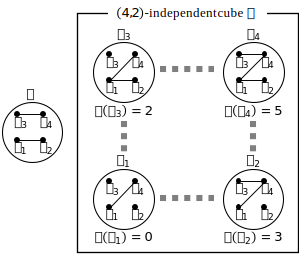
\includegraphics[width=0.9\linewidth]{fig/IndCube.pdf}
  \caption{
    $(4,2)$-independent cube $\calA$ for $f$. 
    In this example, $M = \{(v_1,v_2),(v_3,v_4)\}$, $G_1=(V,E)$, $\calA = \{(V, E \cup N): N \subseteq M\}$, 
    $C_{(v_1,v_2)}=2$, and $C_{(v_3,v_4)}=3$.
    %Definition~\ref{chap1-def:mono-cube} requires that $f$ increase by at least $D=2$ along the dotted gray lines, which it does.
    Adding $(v_1,v_2)$ and $(v_3,v_4)$ increase $f$ by $2$ and $3$, respectively.
  }\label{chap1-fig:mono-cube}
\end{figure}

\begin{figure}[t]
  \centering
  %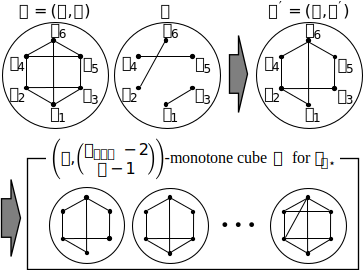
\includegraphics[width=0.88\linewidth]{fig/MonoCube_kstar.pdf}
  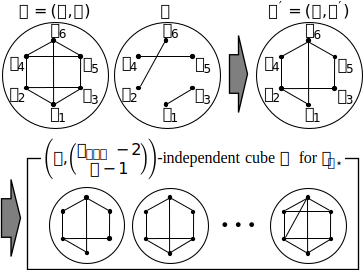
\includegraphics[width=0.9\linewidth]{fig/IndCube_kstar.pdf}
  \caption{
    Construction of an independent cube for a $k$-star function ($n=6$, $d_{max}=4$). 
    From a 
    %$(d_{max} - 1)$-
    $3$-regular graph $G=(V,E)$ and $M=\{(v_1,v_3),(v_2,v_6),(v_4,v_5)\}$, we make a graph $G'=(V,E')$ such that $E' = E \setminus M$. 
    Then $\calA = \{(V, E' \cup N): N \subseteq M\}$ forms an
    $(n, 2\binom{d_{max}-2}{k-1})$-independent cube for $f_{k\star}$.
  }\label{chap1-fig:mono-cube_kstar}
\end{figure}

% We show how to construct an $(n, \binom{d_{max}-3}{k-1})$ monotone cube
% $\mathcal{A}_{k\star}$ for
% $f_{k\star}$. First, we have to take care of a technicality.
% Note that $f_{k\star}(\bmA)$ only operates on symmetric graphs. We extend it to 
% general graphs in a natural way: let $f_{k\star}^{ext}(\bmA)$
% count the number of pointed-out $k$-stars in $\bmA$. Let
% $sym(\mathcal{A})$ be only those matrices in $\mathcal{A}$ that are symmetric,
% corresponding to undirected graphs. We show in the Appendix
% that if $\hf$ privately estimates $f_{k\star}^{ext}$ in the one-round
% edge LDP model, then there is a private estimator $\hat{g}$ that estimates
% $f_{k\star}$ in the one-round edge-LDP model such that
% \begin{multline}\label{chap1-eq:sym-lower-bound}
%   \E_{\bmA \sim U(\mathcal{A}_{k\star})}[l_2^2(f^{ext}_{k\star}(\bmA),
%   \hf(\bmA))] \\ \leq 
%   \E_{\bmA \sim U(sym(\mathcal{A}_{k\star}))} [l_2^2(f_{k\star}(\bmA),
%   \hf(\bmA))] + O(D^2)
% \end{multline}

Such a set of inputs has an ``independence'' property because,
regardless of which edges from $M$ has been added before, adding edge $e \in M$
always changes $f$ by $C_e$. 
Figure~\ref{chap1-fig:mono-cube} shows an example of a $(4,2)$-independent cube for $f$. 

% For example, 
We can also construct 
% an
% Our 
% $(n,\binom{d_{max}-3}{k-1})$ 
% $(n,\binom{d_{max}-4}{k-1})$ 
a independent cube for 
a $k$-star function 
% on directed graphs 
as follows. 
% $f_{k\star}^{ext}$ is the
% following:
% Assume $d_{max}$ and $n$ are both even. 
Assume that $n$ is even. 
It is well known in graph theory that if $n$ is even, then 
for any $d\in[n-1]$, there exists a 
$d$-regular graph where every node has degree $d$ \cite{Ganesan_arXiv18}. 
%Assume $n$ and $d_{max}$ are even and 
Therefore, there exists a 
% Let $G \in \calG$ be a $(d_{max}-1)$-regular graph 
$(d_{max}-1)$-regular graph $G=(V,E)$ 
of size $n$. 
% or a graph 
% in which every node has degree $d_{max}-1$. 
% It is a standard result in graph theory that 
% for any $d\in[n-1]$, 
% $d$-regular graphs exist 
% % for all $d$ 
% when $n$ is even.
Pick an arbitrary perfect matching $M$ on the nodes. Now, let 
% $G' = G \setminus M$. 
$G' = (V,E')$ such that $E' = E \setminus M$. 
Every node in $G'$ has degree between $d_{max}-2$ and $d_{max}-1$. 
Adding an edge in $M$ to $G'$ will produce at least
$2\binom{d_{max}-2}{k-1}$ new $k$-stars.
%the resulting graph be $\bmA = \{\bma_1,\ldots, \bma_n\}$.
%The collection $\prod_{i=1}^n \{\bma_i, \bma_i'\}$ (where the product is the Cartesian product) 
%forms an
% $(n,\binom{d_{max}-3}{k-1})$ 
% $(n,\binom{d_{max}-4}{k-1})$ 
Thus, $\calA = \{(V, E' \cup N): 
% G' \cup N : 
N \subseteq M\}$ forms an
$(n, 2\binom{d_{max}-2}{k-1})$-independent cube for $f_{k\star}$. 
% for $f_\triangle^{ext}$ 
% $\binom{d_{max}-3}{k-1}$ 
% $\binom{d_{max}-4}{k-1}$ 
%Similarly, for even natural number $l \in \nats$ such that $d_{max}>l+2$, we can construct an $(n,\binom{d_{max}-l-2}{k-1})$ monotone cube from the adjacency matrix of a collection of cliques of size $d_{max}-l$.
Note that the maximum degree of each graph in $\calA$ is at most $d_{max}$. 
Figure~\ref{chap1-fig:mono-cube_kstar} shows how to construct an independent cube for a $k$-star function when $n=6$ and $d_{max}=4$. 

% Let $U(\mathcal{A})$ be the uniform distribution over an $(n,D)$ monotone cube $\mathcal{A}$. 
Using the structure that the $(n,D)$-independent cube imposes on $f$,
we can prove a lower bound:
\begin{theorem}\label{chap1-thm:lower-bound}
  Let 
  %$\hf(\bmA)$ 
  $\hf(G)$ 
  have the form of~\eqref{chap1-eq:one-round-lower}, 
  where $\calR_1, \ldots, \calR_n$ are independently run.
  %Assume that 
  %$(\calR_1, \ldots, \calR_n)$ 
  %satisfy 
  %provide 
  %$\epsilon$-relationship DP. 
  %and are independently run.
  Let $\cal{A}$ be an $(n,D)$-independent cube for $f$. 
  If 
  $(\calR_1, \ldots, \calR_n)$ 
  provides 
  $\epsilon$-relationship DP, 
  then 
  %, with 
  %$\bmA$ 
  %$G$ 
  %uniformly drawn from $\calA$, 
  we have
  \[
    % \E_{\bmA, \calR_1, \ldots, \calR_n}[l_2^2(f(\bmA), \hf(\bmA))] =
    % \Omega(\frac{e^{\epsilon}}{(e^{\epsilon}+1)^2}nD^2).
    \frac{1}{\calA} \sum_{G \in \calA} \E[l_2^2(f(G), \hf(G))] =
    \Omega\left(\frac{e^{\epsilon}}{(e^{\epsilon}+1)^2}nD^2\right).
  \]
\end{theorem}

% \begin{corollary}\label{chap1-cor:lower-bound2}
%   If $\hf$ satisfies $\epsilon$-edge LDP in the one-round model, then $\E_{\bmA \sim U(\mathcal{A})}[l_2^2(f(\bmA), \hf(\bmA))] =
%   \Omega(\min\{1, \frac{e^{4\epsilon}}{(e^{4\epsilon}-1)^2}\}nD^2)$.
% \end{corollary}

A corollary of Theorem~\ref{chap1-thm:lower-bound} is that if $\calR_1, \ldots,
\calR_n$ satisfy $\epsilon$-edge LDP, then they satisfy $2\epsilon$
-relationship DP and thus for edge LDP we have a lower bound of
$\Omega\left(\frac{e^{2\epsilon}}{(e^{2\epsilon}+1)^2}nD^2\right)$.
% predictor $\hf$ predicting the average $\E_{\bmA \sim U(\mathcal{A})}[f(\bmA)]$
% will satisfy $\E_{\bmA \sim U(\mathcal{A})}[l_2^2(f(\bmA), \hf(\bmA))] =
% O(nD^2)$ regardless of $\epsilon$. To overcome this problem, one would have to 
% consider a different input structure for $f$ than the $(n,D)$ monotone cube, 
% but we leave this for future work.

Theorem~\ref{chap1-thm:lower-bound}, combined with the fact that there exists an
% $(n,\binom{d_{max}-2}{k-1})$ 
$(n,2\binom{d_{max}-2}{k-1})$-independent cube for 
a $k$-star function 
% $f_{k\star}$ 
% and~\eqref{chap1-eq:sym-lower-bound}, 
implies Corollary~\ref{chap1-cor:kstars-lb}. 
% (see Appendix~\ref{chap1-sub:proof_cor_kstars-lb} for details).
In Appendix~\ref{chap1-sub:cube_triangle}, we also construct an $(n, \frac{d_{max}}{2}-2)$
independent cube 
for $f_\triangle$ and establish a lower bound of 
$\Omega(\frac{e^{2\epsilon}}{(e^{2\epsilon}+1)^2} nd_{max}^2)$ for
$f_\triangle$. 

The upper and lower bounds on the $l_2$ losses 
% for the central,
% local non-interactive, 
% one-round local, 
% and 
% local sequentially interactive 
% two-rounds local 
% models discussed 
shown in
this section appear in Table~\ref{chap1-tab:perf}.

\section{Double Clipping}
\label{chap2-sec:double_clip}

% However, 
% all of our three algorithms still suffer from a very large estimation error. due to a large amount of the Laplacian noise. 
In Section~\ref{chap2-sec:algorithms}, 
% \ref{chap2-sub:algorithms_theoretical_analysis}, 
we showed that the estimation error caused by empirical estimation (i.e., the first term in Theorem~\ref{chap2-thm:l2loss_algorithms}) is significantly reduced by the $4$-cycle trick. 
However, 
% all of the upper-bounds in 
the estimation error is 
% caused by the Laplacian noise (i.e., the second term)  
% Theorem~\ref{chap2-thm:l2loss_algorithms} are 
still very large in our algorithms presented in Section~\ref{chap2-sec:algorithms}, as shown in our experiments. 
% due to a large amount of the Laplacian noise (as shown in our experiments). 
% In particular, 
This is because 
the estimation error by the Laplacian noise (i.e., the second term in Theorem~\ref{chap2-thm:l2loss_algorithms}) 
% the Laplacian noise 
is very large, especially for small $\epsilon_2$ or 
% $\mu_F$ ($=\mu_O^2 = \mu_T^3$), 
$\mu$. 
% as shown in Theorem~\ref{chap2-thm:l2loss_algorithms}. 
% In Section~\ref{chap2-sec:double_clip}, we introduce a double clipping technique to significantly reduce the amount of Laplacian noise.
This error term is tight and unavoidable as long as we use $d_{max}$ as a global sensitivity, which suggests that we need a better global sensitivity analysis.
% In 
% Section~\ref{chap2-sec:double_clip}, 
% the next section, 
% we introduce \textit{double clipping} to significantly reduce the amount of Laplacian noise.
% 
% Our three algorithms in Section~\ref{chap2-sec:algorithms} suffer from a large amount of the Laplacian noise. 
% due to the large global sensitivity. 
% To address this issue, 
% Thus, we propose a double clipping technique, which significantly reduces the global sensitivity of the Laplacian noise. 
To significantly reduce the global sensitivity, we propose a novel \textit{double clipping} technique. 
% Therefore, we propose a double clipping technique, which significantly reduces the global sensitivity of the Laplacian noise. 

We describe the overview and details of our double clipping in Sections~\ref{chap2-sub:clip_overview} and \ref{chap2-sub:algorithms}, respectively. 
Then we perform theoretical analysis in Section~\ref{chap2-sub:clip_theoretical_analysis}.

\subsection{Overview}
\label{chap2-sub:clip_overview}

% \smallskip
\noindent{\textbf{Motivation.}}~~Figure~\ref{chap2-fig:reduce_noisy_triangles} shows noisy triangles involving edge $(v_i,v_j)$ counted by user $v_i$ in our three algorithms. 
Our algorithms in Section~\ref{chap2-sec:algorithms} 
% (and the two-rounds algorithm in \cite{Imola_USENIX21}) 
use the fact that the number of such noisy triangles (hence the global sensitivity) is upper-bounded by the maximum degree $d_{max}$ because 
%user $v_i$'s degree is at most $d_{max}$). 
adding one edge increases the triangle count by at most $d_{max}$. 
Unfortunately, this upper-bound is too large, as shown in our experiments. 
% Although this is correct, we 

% Our basic idea is that we can 
In this paper, we 
significantly reduce this upper-bound by using the parameter $\mu$ in the ARR and user $v_i$'s degree $d_i \in \nnints$ for users with smaller IDs. 
For example, 
% we can expect that 
the number of noisy triangles involving $(v_i,v_j)$ in \AlgOne is 
expected to be around 
$\mu d_i$ 
% ($\mu \ll 1$, $d_i < d_{max}$) 
% with high probability (larger than $0.5$) 
because one noisy edge is included in each noisy triangle (as shown in Figure~\ref{chap2-fig:reduce_noisy_triangles}) and all noisy edges are independent. 
$\mu d_i$ is very small, especially when we set $\mu \ll 1$ to reduce the communication cost.  
% Similarly, the expected number of noisy triangles involving $(v_i,v_j)$ in \AlgTwo is $\mu_O^2 d_i$ because two independent noisy edges are in each noisy triangle (as in Figure~\ref{chap2-fig:reduce_noisy_triangles}).

However, we cannot directly use $\mu d_i$ as an upper-bound of the global sensitivity in \AlgOne for two reasons. 
First, $\mu d_i$ leaks the exact value of user $v_i$'s degree $d_i$ 
and 
% , hence 
violates edge LDP. 
% friendship information of $v_i$ (e.g., as an extreme example, $d_i=0$ reveals the fact that $v_i$ has no friends). 
Second, the number of noisy triangles involving $(v_i,v_j)$ exceeds $\mu d_i$ with high probability (about $0.5$). 
Thus, the noisy triangle count cannot be upper-bounded by $\mu d_i$. 

\begin{figure}[t]
  \centering
  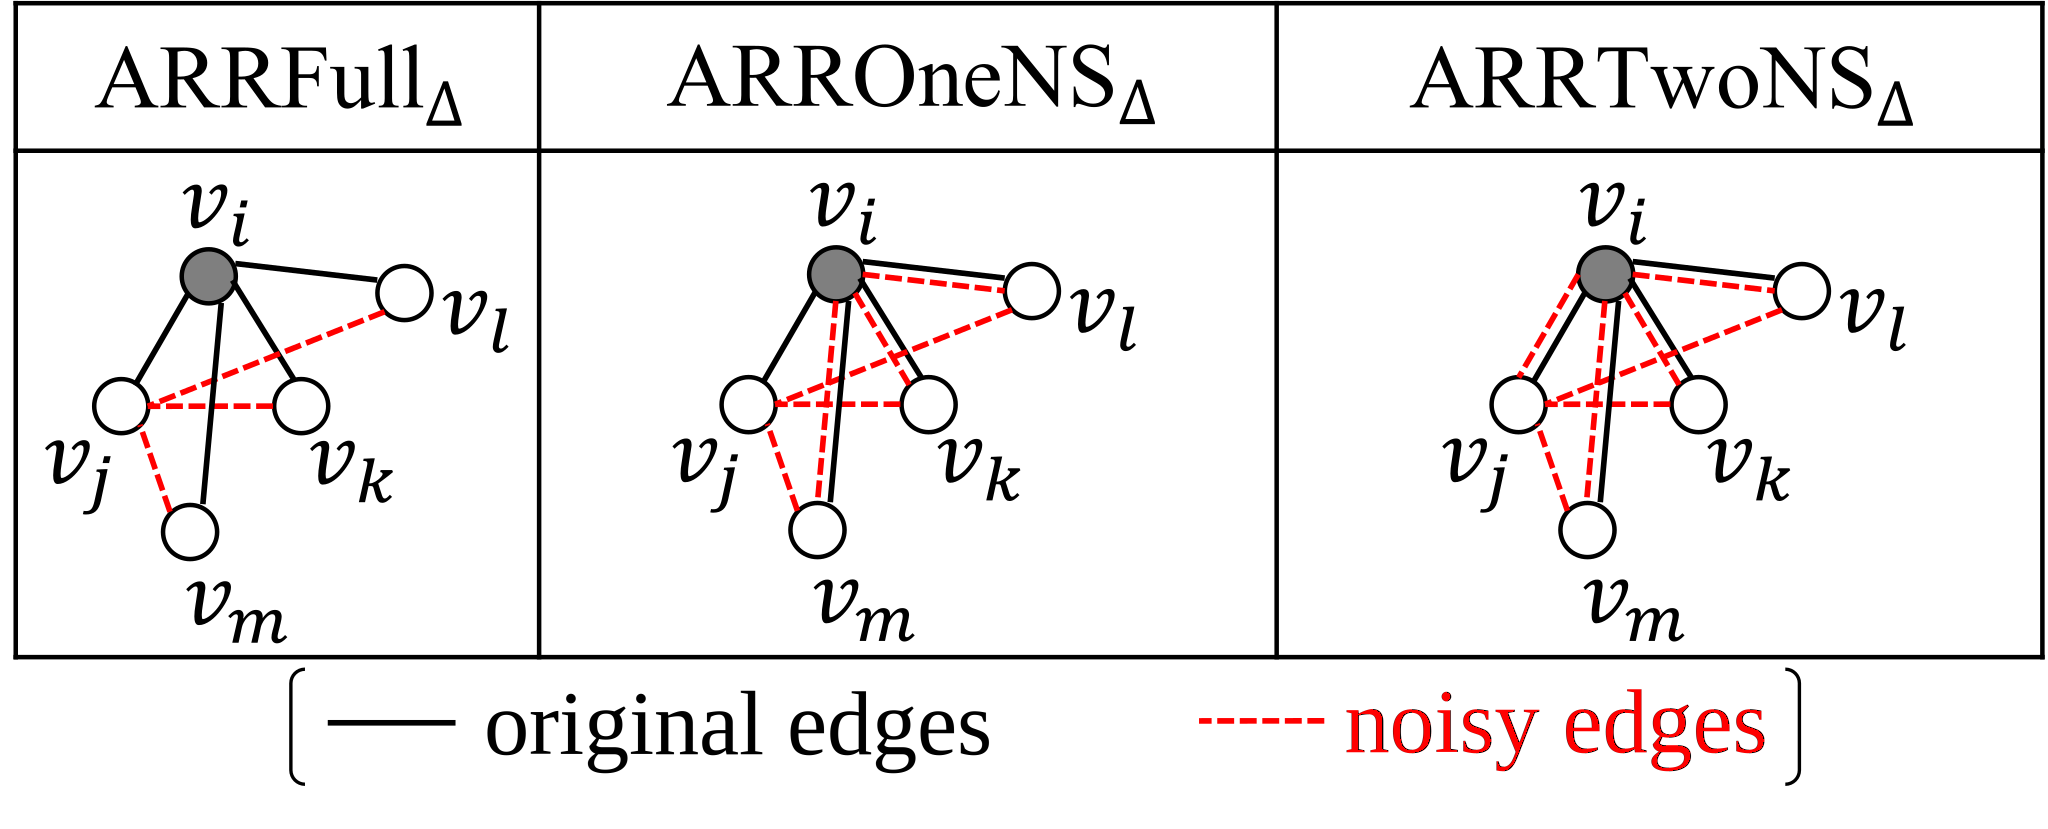
\includegraphics[width=0.78\linewidth]{fig/double_clipping.pdf}
  
  \caption{Noisy triangles involving edge $(v_i,v_j)$ counted by user $v_i$ ($j<k,l,m<i$).} 
  \label{chap2-fig:reduce_noisy_triangles}
%\end{figure}
\vspace{2mm}
%\begin{figure}[t]
  \centering
  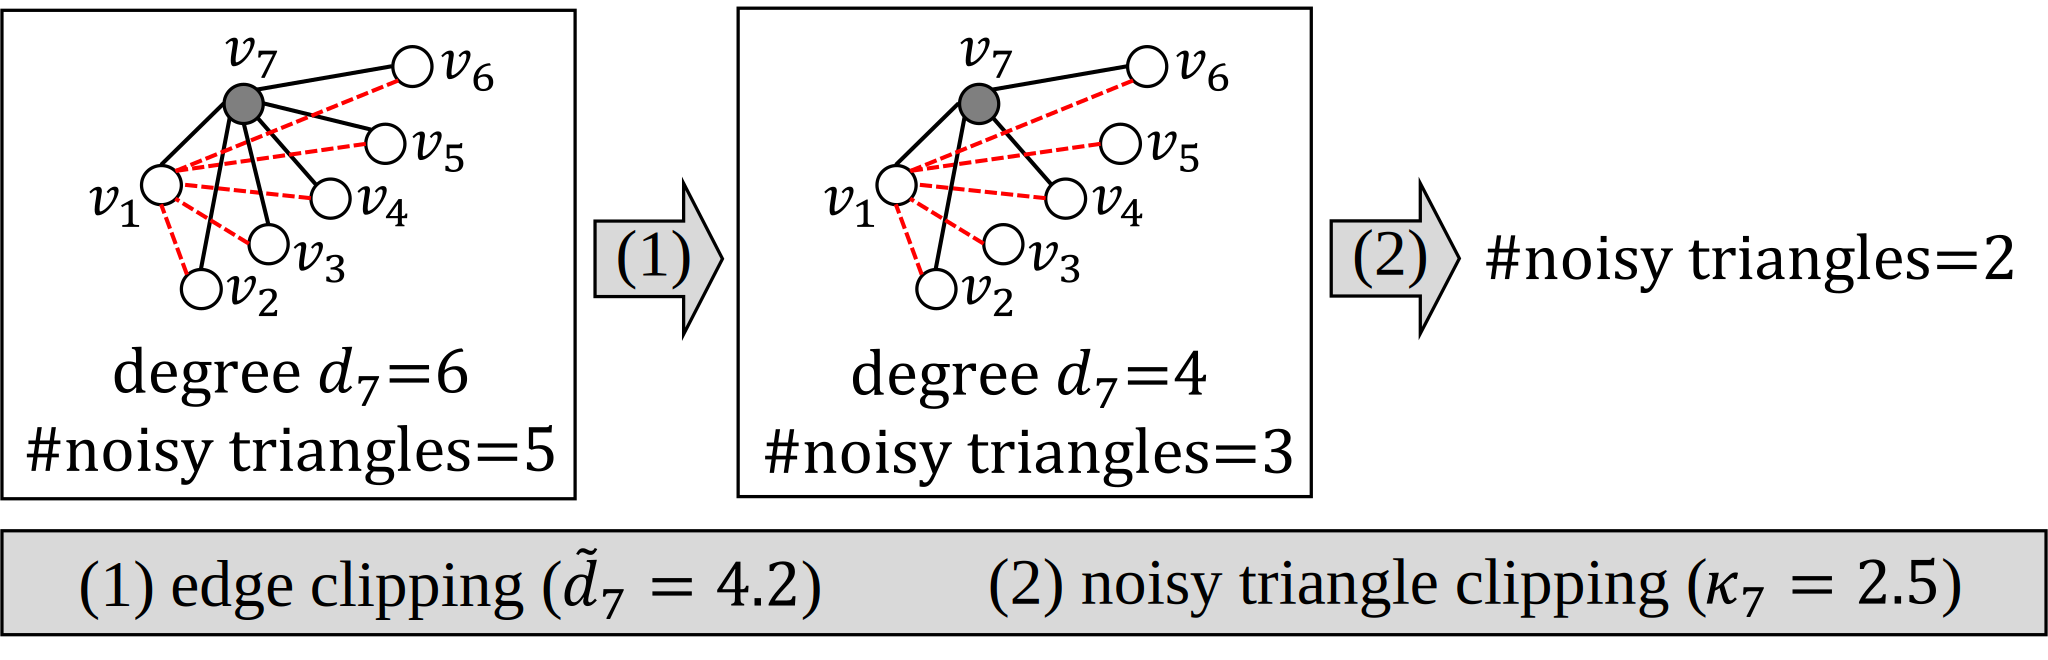
\includegraphics[width=0.99\linewidth]{fig/clip_overview.pdf}
  
  \caption{Overview of double clipping applied to edge ($v_1,v_7$).} 
  \label{chap2-fig:double-clip_overview}
\end{figure}

% To address the first and second issues explained above, we introduce an edge clipping and triangle clipping, respectively. 
To address these two issues, 
%(i.e., the leakage of $d_i$ and the excess of the noisy triangle count), 
we propose a double clipping technique, which is explained below. 
% which consists of an \textit{adaptive edge clipping} and \textit{noisy triangle clipping}. 

\smallskip
\noindent{\textbf{Algorithm Overview.}}~~Figure~\ref{chap2-fig:double-clip_overview} shows 
% its overview. 
the overview of our double clipping, which consists of an 
% \textit{adaptive edge clipping} 
\textit{edge clipping} 
and \textit{noisy triangle clipping}. 
% The adaptive edge clipping 
The edge clipping 
addresses the first issue (i.e., leakage of $d_i$) 
as follows. 
% by borrowing the idea of adaptive clipping \cite{Andrew_arXiv21,Pichapati_arXiv19} 
% in DP-SGD (Differentially Private Stochastic Gradient Descent). 
% which privately estimates an appropriate clipping threshold in DP-SGD (Stochastic Gradient Descent) \cite{Abadi_CCS16} with DP. 
% Specifically, it 
It privately computes 
a noisy version of 
$d_i$ (denoted by $\td_i$) with edge LDP. 
% Let $\td_i \in \nnreals$ be the private value of $d_i$. 
% user $v_i$ 
% adds the Laplacian noise and some positive constant $\eta \in \nnreals$ to $d_i$ to provide edge LDP 
% and 
Then it 
%performs edge clipping 
%(a.k.a. graph projection \cite{Day_SIGMOD16,Ding_TKDE21,Kasiviswanathan_TCC13,Raskhodnikova_arXiv15}), which 
removes some neighbors from a neighbor list $\bma_i$ so that the degree of $v_i$ never exceeds 
% the private estimate of $d_i$. 
% the private value of $d_i$ 
% (denoted by $\td_i \in \nnreals$). 
% (denoted by $\td_i$). 
the noisy degree $\td_i$. 
This removal process is also known as graph projection \cite{Day_SIGMOD16,Ding_TKDE21,Kasiviswanathan_TCC13,Raskhodnikova_arXiv15}. 
% This kind of technique is called adaptive clipping \cite{Andrew_arXiv21,Pichapati_arXiv19} 
% in DP-SGD (Stochastic Gradient Descent) \cite{Abadi_CCS16} because it privately estimates an appropriate clipping threshold with DP. 
% Adaptive edge clipping 
Edge clipping 
is 
% also 
used in \cite{Imola_USENIX21} to obtain a 
% private value of 
noisy version of 
% the maximum degree 
$d_{max}$. 
%(though ours is to obtain a noisy version of $d_i$). 

% The triangle clipping addresses the second issue (i.e., excess of the noisy triangle count) by reducing the noisy triangle count so that it never exceeds a 
% user-dependent threshold $\kappa_i \in \nnints$. 
The main novelty in our double clipping lies at the \textit{noisy triangle clipping} to address the second issue (i.e., excess of the noisy triangle count). 
% Note that 
This issue appears 
% only 
when 
% each edge is sampled and 
we attempt to reduce the global sensitivity by using 
a very small sampling probability for each edge. 
% value of $\mu$ in the ARR.  
% using a stochastic algorithm such as the ARR. 
Therefore, the noisy triangle clipping has not been studied in the existing works on private triangle counting 
% \cite{Ding_TKDE21,Imola_USENIX21,Karwa_PVLDB11,Kasiviswanathan_TCC13,Song_arXiv18,Sun_CCS19,Ye_ICDE20,Ye_TKDE21,Zhang_SIGMOD15}, 
\cite{Ding_TKDE21,Imola_USENIX21,Karwa_PVLDB11,Kasiviswanathan_TCC13,Sun_CCS19,Ye_ICDE20,Ye_TKDE21,Zhang_SIGMOD15}, 
because they do not apply a sampling technique. 

Our noisy triangle clipping reduces the noisy triangle count so that it never exceeds a 
user-dependent clipping threshold 
$\kappa_i \in \nnreals$. 
% $\kappa_i = \lambda_i \mu^* \td_i$, where $\lambda_i \in \nats$. 
% We call $\kappa_i$ and $\lambda_i$ the \textit{clipping threshold} and \textit{clipping coefficient}, respectively. 
Then a crucial issue is how to set 
an appropriate 
% clipping 
threshold 
$\kappa_i$. 
We theoretically analyze the probability that the noisy triangle count exceeds $\kappa_i$ 
(referred to as the \textit{triangle excess probability}) 
as a function of 
the ARR parameter $\mu$ and the 
% private value $\td_i$ of $d_i$. 
noisy degree $\td_i$. 
% of user $v_i$. 
Then we set $\kappa_i$ so that 
the triangle excess probability 
% the probability 
is very small ($=10^{-6}$ in our experiments). 

We use the clipping threshold $\kappa_i$ as a global sensitivity. 
% of the Laplacian noise. 
Note that $\kappa_i$ provides edge LDP because $\td_i$ provides edge LDP, 
% and $\kappa_i$ depends on only $\mu$ and $\td_i$ 
i.e., immunity to post-processing \cite{DP}. 
$\kappa_i$ is also very small when $\mu \ll 1$, as it is determined based on $\mu$. 

% We also emphasize that our double clipping does \textit{not} assume that $d_{max}$ is public, because it privately computes $\td_i$. 
% by adaptive edge clipping.

\subsection{Algorithms}
\label{chap2-sub:algorithms}
Algorithm~\ref{chap2-alg:clip} shows our double clipping algorithm. 
All the processes are run by user $v_i$ at the second round. 
Thus, there is no interaction with the server in Algorithm~\ref{chap2-alg:clip}.

\setlength{\algomargin}{5mm}
\begin{algorithm}[t]
  \SetAlgoLined
  \KwData{Neighbor list $\bma_i \in \{0,1\}^n$, privacy budget
  $\epsilon_0 \in \nnreals$ 
  $\mu \in [0,\frac{e^{\epsilon_1}}{e^{\epsilon_1} + 1}]$, 
  %$\eta \in \nnreals$.
  $\alpha \in \nnreals$, 
  $\beta \in \nnreals$.
  }
  \KwResult{$\hw_i$.}
  $\mu^* \leftarrow \mu$, $\mu^2$, and $\mu^3$ in F, O, and T, respectively\;
  \tcc{Edge clipping.}
  %$\td_i = \max\{d_i + \Lap(\frac{1}{\epsilon_0}) + \eta$, 0\}\;
  $\td_i = \max\{d_i + \Lap(\frac{1}{\epsilon_0}) + \alpha$, 0\}\;
  \tcc{Remove $d_i - \lfloor \td_i \rfloor$ neighbors if $d_i > \td_i$.}
  $\bma_i \leftarrow \texttt{GraphProjection}(\bma_i, \td_i)$\;
  \tcc{Noisy triangle clipping.}
  \For{$j$ \rm{such that} $a_{i,j} = 1$ \rm{and} $j<i$}{
    $t_{i,j} \leftarrow |\{(v_i,v_j,v_k) : a_{i,k} = 1, (v_j,v_k) \in M_i, j<k<i \}|$\;
  }
%  \tcc{Calculate $\kappa_i$ such that $\kappa_i \in [\mu^* \td_i, \td_i]$.}
   \tcc{Calculate $\kappa_i \in [\mu^* \td_i, \td_i]$ s.t. the triangle excess probability is $\beta$ or less.}
%  \tcc{Calculate $\lambda_i \in \nats$ such that the triangle excess probability is $\beta$ or less.}
  $\kappa_i \leftarrow \texttt{ClippingThreshold}(\mu, \td_i, \beta)$\;
%  $\lambda_i \leftarrow \texttt{ClippingThreshold}(\mu, \td_i, \beta)$\;
%   $\kappa_i \leftarrow \lambda_i \mu^* \td_i$\;
  $t_i \leftarrow \sum_{a_{i,j} = 1, j<i} \min \{t_{i,j}, \kappa_i\}$\;
  $s_i \leftarrow |\{(v_i,v_j,v_k) : a_{i,j} = a_{i,k} = 1, j<k<i\}|$\;
  $w_i \leftarrow t_i - \mu^* \rho s_i$\;
  $\hw_i \leftarrow w_i + \Lap(\frac{\kappa_i}{\epsilon_2})$\;
  \KwRet{$\hw_i$}
  \caption{Our double clipping algorithm. 
  ``F'', ``O'', ``T'' are shorthands for 
  \AlgOne{}, \AlgTwo{}, and \AlgThree{}, respectively.
  All the processes are run by user $v_i$.
  }\label{chap2-alg:clip}
\end{algorithm}

\smallskip
\noindent{\textbf{Edge Clipping.}}~~The edge clipping appears in lines 2-3 of Algorithm~\ref{chap2-alg:clip}. 
It uses a privacy budget $\epsilon_0 \in \nnreals$. 
% for privately computing $d_i$. 

In line 2, user $v_i$ adds the Laplacian noise $\Lap(\frac{1}{\epsilon_0})$ to her degree $d_i$. 
Since adding/removing one edge changes $d_i$ by at most $1$, this process provides $\epsilon_0$-edge LDP. 
$v_i$ also adds some non-negative constant 
% $\eta \in \nnreals$ 
$\alpha \in \nnreals$ 
to $d_i$. 
We add this value so that edge removal (in line 3) occurs with a very small probability; 
e.g., in our experiments, we set $\alpha = 150$, where 
% when $\epsilon_0 = 0.1$ and $\alpha = 150$, 
edge removal occurs with probability $1.5 \times 10^{-7}$ when $\epsilon_0 = 0.1$. 
A similar technique is introduced in \cite{Sun_CCS19} to provide ($\epsilon, \delta)$-DP \cite{DP} with small $\delta$. 
The difference between ours and \cite{Sun_CCS19} is that we perform edge clipping 
% (graph projection) 
to always provide $\epsilon$-DP; i.e., $\delta = 0$.
Let $\td_i \in \nnreals$ be the noisy degree of $v_i$.

In line 3, user $v_i$ calls the function \texttt{GraphProjection}, which performs graph projection as follows; 
if $d_i > \td_i$, randomly remove $d_i - \lfloor \td_i \rfloor$ neighbors from $\bma_i$; otherwise, do nothing. 
Consequently, the degree 
% $d_i$ 
of $v_i$ never exceeds $\td_i$. 

\begin{table*}[t]
  \centering
	\rotatebox{270}{
  \begin{tabular}{|l|c|c|c|}
    \hline
    & \AlgOne & \AlgTwo & \AlgThree \\ \hline
    Privacy 
    & \multicolumn{3}{|c|}{$(\epsilon_0 + \epsilon_1 + \epsilon_2)$-edge LDP and $(\epsilon_0 + \epsilon_1 + \epsilon_2)$-relationship DP} \\ \hline
    %& $\epsilon_0 + \epsilon_1 + \epsilon_2$ & $\epsilon_0 + \epsilon_1 + \epsilon_2$ &
    %$\epsilon_0 + \epsilon_1 + \epsilon_2$ \\ \hline
    Expected $l_2$ loss 
    % & $\frac{2 C_4(G) + S_2(G)}{\mu(1-e^{-\epsilon_1})^2}$ + $\frac{2 \sum_{i=1}^n \kappa_{i}^2}{\mu^2 (1-e^{-\epsilon_1})^2 \epsilon_2^2}$
    % & $O\left(\frac{n d_{max}^3}{\mu(1-e^{-\epsilon_1})^2} + \frac{2 \sum_{i=1}^n \lambda_{i}^2 \td_i^2}{(1-e^{-\epsilon_1})^2 \epsilon_2^2}\right)$
    & $O\left(\frac{n d_{max}^3}{\mu(1-e^{-\epsilon_1})^2} + \frac{2 \sum_{i=1}^n \kappa_{i}^2}{\mu^2(1-e^{-\epsilon_1})^2 \epsilon_2^2}\right)$
    % & $\frac{\mu(12 S_3(G) + 6 P_3(G)) + 6 S_2(G)}{\mu^2(1-e^{-\epsilon_1})^2}$ + $\frac{2 \sum_{i=1}^n \kappa_{i}^2}{\mu^4 (1-e^{-\epsilon_1})^2 \epsilon_2^2}$
    % & $O\left(\frac{n d_{max}^2}{\mu^2(1-e^{-\epsilon_1})^2} + \frac{2 \sum_{i=1}^n \lambda_{i}^2 \td_i^2}{(1-e^{-\epsilon_1})^2 \epsilon_2^2} \right)$
    & $O\left(\frac{n d_{max}^2}{\mu^2(1-e^{-\epsilon_1})^2} + \frac{2 \sum_{i=1}^n \kappa_{i}^2}{\mu^4 (1-e^{-\epsilon_1})^2 \epsilon_2^2} \right)$
    % & $\frac{\mu^2 (12 S_3(G) + 6 P_3(G)) + 6 S_2(G)}{\mu^3(1-e^{-\epsilon_1})^2}$ + $\frac{2 \sum_{i=1}^n \kappa_{i}^2}{\mu^6 (1-e^{-\epsilon_1})^2 \epsilon_2^2}$ \\ \hline
    % & $O\left(\frac{n d_{max}^2}{\mu^3(1-e^{-\epsilon_1})^2} + \frac{2 \sum_{i=1}^n \lambda_{i}^2 \td_i^2}{(1-e^{-\epsilon_1})^2 \epsilon_2^2} \right)$ \\ \hline
    & $O\left(\frac{n d_{max}^2}{\mu^3(1-e^{-\epsilon_1})^2} + \frac{2 \sum_{i=1}^n \kappa_{i}^2}{\mu^6 (1-e^{-\epsilon_1})^2 \epsilon_2^2} \right)$ \\ \hline
    % $l_2$ loss of emp 
    % & $\frac{2 C_4(G) + S_2(G)}{\mu_F(1-e^{-\epsilon_1})^2}$
    % & $\frac{\mu_O(12 S_3(G) + 6 P_3(G)) + 6 S_2}{\mu_O^2(1-e^{-\epsilon_1})^2}$
    % & $\frac{\mu_T^2 (12 S_3(G) + 6 P_3(G)) + 6 S_2}{\mu_T^3(1-e^{-\epsilon_1})^2}$ \\ \hline
    % $l_2$ loss of \Lap{} 
    % & $\frac{2 \sum_{i=1}^n \kappa_{i,F}^2}{\mu_F^2 (1-e^{-\epsilon_1})^2 \epsilon_2^2}$
    % & $\frac{2 \sum_{i=1}^n \kappa_{i,O}^2}{\mu_F^2 (1-e^{-\epsilon_1})^2 \epsilon_2^2}$
    % & $\frac{2 \sum_{i=1}^n \kappa_{i,T}^2}{\mu_F^2 (1-e^{-\epsilon_1})^2 \epsilon_2^2}$ \\ \hline
    $\text{Cost}_{DL}$ & 
    $\mu n^2 \log n$ 
    % $\mu e^{-\epsilon_1} n^2 \log n$ 
    % $\mu_F e^{-\epsilon_1} n(n-1) \log n$ 
    % $(n(n-1) \mu_F \rho + |E| \mu_F (1 - \rho)) \log n$ 
    & 
    $\mu^2 n^2 \log n$ 
    % $\mu^2 e^{-\epsilon_1} n^2 \log n$ 
    % $\mu_O^2 e^{-\epsilon_1} n(n-1) \log n$ 
    & 
    $\mu^3 n^2 \log n$ 
    % $\mu^3 e^{-\epsilon_1} n^2 \log n$ 
    % $\mu_T^3 e^{-\epsilon_1} n(n-1) \log n$ 
    \\ \hline
    $\text{Cost}_{UL}$ & 
    $\mu n \log n$ & $\mu n \log n$ & $\mu n \log n$ 
    % $\mu e^{-\epsilon_1} n \log n$ & $\mu e^{-\epsilon_1} n \log n$ & $\mu e^{-\epsilon_1} n \log n$ 
    \\ \hline
  \end{tabular}
	}	
  \caption{Performance guarantees 
  %Privacy, expected $l_2$ loss, and download/upload cost 
  of our three algorithms with double clipping when the edge removal and triangle removal do not occur. 
  %($C_4$: \#$4$-cycles, $P_3$: \#$3$-paths, $S_k$: \#$k$-stars). 
  %($\lambda_i$: clipping coefficient, $\td_i$: noisy degree).
  The expected $l_2$ loss assumes that $\mu$ is small. 
  The download (resp.~upload) cost is an upper-bound in (\ref{chap2-eq:CostDL_F}) 
  %, (\ref{chap2-eq:CostDL_O}), (\ref{chap2-eq:CostDL_T}), 
  (resp.~(\ref{chap2-eq:CostUL_proposal})).
  %approximation when $d_{max} \ll n$. 
  %the graph $G$ is sparse.
  }
  \label{chap2-tab:privacy_utility_cost}
\end{table*}

\smallskip
\noindent{\textbf{Noisy Triangle Clipping.}}~~The noisy triangle clipping appears in lines 4-11 of Algorithm~\ref{chap2-alg:clip}. 

% First, 
In lines 4-6, 
user $v_i$ calculates the number $t_{i,j} \in \nnints$ of noisy triangles ($v_i, v_j, v_k$) ($j<k<i$) involving $(v_i,v_j)$ 
(as shown in Figure~\ref{chap2-fig:reduce_noisy_triangles}). 
%such that only one edge ($v_j, v_k$) is noisy 
% for her neighbor $v_j$. 
% (lines 4-6). 
Note that the total number $t_i$ of noisy triangles of $v_i$ can be expressed as: 
$t_i = \sum_{a_{i,j}=1, j<i} t_{i,j}$. 
In line 7, $v_i$ calls the function \texttt{ClippingThreshold}, which calculates a clipping threshold 
% $\kappa_i$ 
$\kappa_i \in [\mu^* \td_i, \td_i]$ 
($\mu^* = \mu$, $\mu^2$, and $\mu^3$ in 
``F'', ``O'', and ``T'', respectively) 
based on the ARR parameter $\mu$ and the noisy degree $\td_i$ so that 
% $\kappa_i \in [\mu^* \td_i, \td_i]$ 
% ($\mu^* = \mu$, $\mu^2$, and $\mu^3$ in 
% ``F'', ``O'', and ``T'', respectively) 
% and 
the triangle excess probability does not exceed some constant $\beta \in \nnreals$. 
% $\kappa_i$ takes a value between $\mu^* \td_i$ and $\td_i$; i.e., $\kappa_i \in [\mu^* \td_i, \td_i]$. 
We explain how to calculate 
% $\kappa_i$ from $\mu$ and $\td_i$ 
the triangle excess probability 
in Section~\ref{chap2-sub:clip_theoretical_analysis}. 
% in detail. 
In line 8, $v_i$ calculates the total number $t_i$ of noisy triangles by summing up $t_{i,j}$, with the exception that $v_i$ adds $\kappa_i$ 
%(rather than $t_{i,j}$) 
if $t_{i,j} > \kappa_i$. 
%$t_{i,j}$ exceeds $\kappa_i$. 
In other words, triangle removal occurs 
% when 
if 
$t_{i,j} > \kappa_i$. 
% Consequently, 
Then, 
the number 
% $t_{i,j}$ 
of noisy triangles involving $(v_i,v_j)$ never exceeds $\kappa_i$. 

Lines 9-11 in Algorithm~\ref{chap2-alg:clip} are the same as lines 12-14 in Algorithm~\ref{chap2-alg:unify}, except that 
the global sensitivity in the former (resp.~latter) is $\kappa_i$ (resp.~$d_{max}$). 
% the global sensitivity in Algorithm~\ref{chap2-alg:clip} is $\kappa_i$. 
Line 11 in Algorithm~\ref{chap2-alg:clip} provides $\epsilon_2$-edge LDP because the number of triangles involving $(v_i,v_j)$ is now upper-bounded by $\kappa_i$. 

\smallskip
\noindent{\textbf{Our Entire Algorithms with Double Clipping.}}~~We can run our algorithms \AlgOne{}, \AlgTwo{}, \AlgThree{} with double clipping just by replacing lines 11-14 in Algorithm~\ref{chap2-alg:unify} with lines 2-11 in Algorithm~\ref{chap2-alg:clip}. 
That is, after calculating $\hw_i$ by Algorithm~\ref{chap2-alg:clip}, $v_i$ uploads $\hw_i$ to the server. 
Then the server calculates an estimate of $f_\triangle(G)$ as $\hf_\triangle(G) = \frac{1}{\mu^*(1-\rho)}\sum_{i=1}^n \hw_i$. 
%as in line 17 of Algorithm~\ref{chap2-alg:unify}. 
% where $\mu^* = \mu$, $\mu^2$, and $\mu^3$ in 
% ``F'', ``O'', and ``T'', respectively). 

We also note that the input $d_{max}$ in Algorithm~\ref{chap2-alg:unify} is no longer necessary thanks to the edge clipping; i.e., our entire algorithms with double clipping do not assume that $d_{max}$ is public. 
% , because $v_i$ privately calculates $d_i$ by edge clipping.

\subsection{Theoretical Analysis}
\label{chap2-sub:clip_theoretical_analysis}
% \paragraph{Privacy}
% \smallskip
We now perform a theoretical analysis on the privacy and utility of our double clipping. 
% All the proofs appear in \arxiv{Appendix~\ref{chap2-sec:proof_double_clip}}\conference{the full version \cite{Imola_arXiv22}}. 

\smallskip
\noindent{\textbf{Privacy.}}~~We begin with the privacy guarantees:
% Our algorithms with double clipping have the following privacy guarantees:
\begin{theorem}\label{chap2-thm:privacy_DC}
  For $i \in [n]$, 
  let $\calR_i^1, \calR_i^2(M_i)$ be the randomizers used by user $v_i$ in
  rounds $1$ and $2$ of our algorithms with double clipping (Algorithms~\ref{chap2-alg:unify} and \ref{chap2-alg:clip}). 
  Let $\calR_i(\bma_i) = (\calR_i^1(\bma_i), \calR_i^2(M_i)(\bma_i))$ 
  be the composition of the two randomizers. 
  Then,
  $\calR_i$ satisfies $(\epsilon_0 + \epsilon_1 + \epsilon_2)$-edge LDP, 
  %for $i \in [n]$, 
  and $(\calR_1,
  \ldots, \calR_n)$ satisfies $(\epsilon_0 + \epsilon_1 + \epsilon_2)$-relationship DP.
\end{theorem}

\smallskip
\noindent{\textbf{Utility.}}~~Next, we show the triangle excess probability: 
% the probability that the noisy triangle count $t_{i,j}$ exceeds $\kappa_i$:

\begin{theorem}\label{chap2-thm:triangle_excess}
%Let $\mu^* = \mu_F$ and $\mu_O^2$ in \AlgOne{} and \AlgTwo{}, respectively. 
%In \AlgOne{} and \AlgTwo{}, 
%In \AlgOne{}, \AlgTwo{}, \AlgThree{}, 
% Let $\mu_F, \mu_O, \mu_T \in [0,\frac{e^{\epsilon}}{e^{\epsilon_1} + 1}]$. 
% For $i \in [n]$, let $\td_i \in \nnreals$ be a noisy degree of user $v_i$ output by edge clipping. 
% Let $\kappa_i$
In Algorithm~\ref{chap2-alg:clip}, the triangle excess probability (i.e., probability that the number of noisy triangles $t_{i,j}$ involving edge $(v_i, v_j)$ exceeds a clipping threshold $\kappa_i$) is:
  \begin{align}
    \hspace{-1mm} \Pr(t_{i,j} > \kappa_i) &\leq \textstyle{\exp \left[-\td_i D \left(\frac{\kappa_i}{\td_i} \parallel \mu \right) \right]} \label{chap2-eq:AlgI_clip_bound} \\
    \hspace{-1mm} \Pr(t_{i,j} > \kappa_i) &\leq \textstyle{\exp \left[-\td_i D \left(\frac{\kappa_i}{\td_i} \parallel \mu^2 \right) \right]} \label{chap2-eq:AlgII_clip_bound}\\
%   \end{align}
%   \begin{align}
    \hspace{-1mm} \Pr(t_{i,j} > \kappa_i) &\leq 
    \textstyle{\mu \exp \left[-\td_i D \left(\frac{\max\{\kappa_i,\mu^2 \td_i\}}{\td_i} \parallel \mu^2 \right) \right]}
    % \begin{cases}
    %     \mu_T \exp \left[-\td_i D \left(\frac{\kappa_i}{\td_i} \parallel \mu_T^2 \right) \right]   &   \mathrm{(if}~ \kappa_i \geq \mu_T^2 \td_i)\\
    %     \mu_T   &   \mathrm{(if}~ \mu_T^3 \td_i \leq \kappa_i < \mu_T^2 \td_i),
    % \end{cases}
    \label{chap2-eq:AlgIII_clip_bound}
  \end{align}
  in \AlgOne{}, \AlgTwo{}, and \AlgThree{}, respectively, 
  where 
  % $\mu^* = \mu_F$ and $\mu_O^2$ in \AlgOne{} and \AlgTwo{}, respectively, and 
  $D(p_1 \parallel p_2)$ is the Kullback-Leibler divergence between two Bernoulli distributions; i.e., 
  %$D(p_1 \parallel p_2) = p_1 \log \frac{p_1}{p_2} + (1-p_1) \log \frac{1-p_1}{1-p_2}$.
  %with $p_1$ and $p_2$:
  %the Bernoulli($p_1$) and Bernoulli($p_2$) distribution; 
\begin{align*}
    \textstyle{D(p_1 \parallel p_2) = p_1 \log \frac{p_1}{p_2} + (1-p_1) \log \frac{1-p_1}{1-p_2}.}
\end{align*}
\end{theorem}
In all of (\ref{chap2-eq:AlgI_clip_bound}), (\ref{chap2-eq:AlgII_clip_bound}), and (\ref{chap2-eq:AlgIII_clip_bound}), we use the Chernoff bound, which is known to be reasonably tight \cite{Arratia_BMB89}. 

\smallskip
\noindent{\textbf{Setting $\kappa_i$.}}~~The function \texttt{ClippingThreshold} in Algorithm~\ref{chap2-alg:clip} sets a clipping threshold $\kappa_i$ of user $v_i$ based on Theorem~\ref{chap2-thm:triangle_excess}. 
Specifically, we set $\kappa_i = \lambda_i \mu^* \td_i$, where $\lambda_i \in \nats$, and calculate $\lambda_i$ as follows. 
We initially set $\lambda_i = 1$ and keep increasing $\lambda_i$ by $1$ 
% initially set $\kappa_i = \mu^* \td_i$ and keep increasing $\kappa_i$ by $\mu^* \td_i$ 
until the upper-bound (i.e., right-hand side of (\ref{chap2-eq:AlgI_clip_bound}), (\ref{chap2-eq:AlgII_clip_bound}), or (\ref{chap2-eq:AlgIII_clip_bound})) is smaller than or equal to the triangle excess probability $\beta$. 
In our experiments, we set $\beta = 10^{-6}$. 
% We call $\lambda_i$ the \textit{clipping coefficient} of $v_i$. 

\smallskip
\noindent{\textbf{Large $\kappa_i$ of \AlgThree{}.}}~~By 
% In our experiments, we set $\mu$ so that $\mu$ in \AlgOne{} is equal to $\mu^2$ in \AlgTwo{} and also equal to $\mu^3$ in \AlgThree{}. 
% Then by 
(\ref{chap2-eq:AlgI_clip_bound}) and (\ref{chap2-eq:AlgII_clip_bound}), the upper-bound on the triangle excess probability is the same between \AlgOne{} and \AlgTwo{}. 
% However, 
In contrast, 
\AlgThree{} has a larger upper-bound. 
For example, 
when $\kappa_i = 15 \mu^* \td_i$, $\mu^* = 10^{-3}$, and $\td_i=1000$, 
the right-hand sides of (\ref{chap2-eq:AlgI_clip_bound}), (\ref{chap2-eq:AlgII_clip_bound}), and (\ref{chap2-eq:AlgIII_clip_bound}) are $2.5 \times 10^{-12}$, $2.5 \times 10^{-12}$, and $3.3 \times 10^{-2}$, respectively. 
Consequently, \AlgThree{} has a larger global sensitivity $\kappa_i$ for the same value of $\beta$.

% \smallskip
% \noindent{\textbf{\AlgTwo{} vs. \AlgThree{}.}}~~Now we explain the reason that \AlgTwo can reduce the global sensitivity more effectively than \AlgThree (as described in Section~\ref{chap2-sub:algorithms_overview}).  
% using Figure~\ref{chap2-fig:reduce_noisy_triangles}. 
% As with \AlgOne, 
We can explain a large global sensitivity $\kappa_i$ of \AlgThree{} as follows. 
The number $t_{i,j}$ of noisy triangles involving $(v_i,v_j)$ in 
\AlgOne{} is expected to be around $\mu d_i$ because one noisy edge is in each noisy triangle (as in Figure~\ref{chap2-fig:reduce_noisy_triangles}) and all noisy edges are independent. 
For the same reason, $t_{i,j}$ in \AlgTwo{} is expected to be around $\mu^2 d_i$.  
% \AlgTwo{} is expected to be around $\mu_O^2 d_i$ because two noisy edges are in each noisy triangle (as in Figure~\ref{chap2-fig:reduce_noisy_triangles}) and all noisy edges are independent. 
% 
However, 
% the number of noisy triangles involving $(v_i,v_j)$ 
$t_{i,j}$ in \AlgThree{} is \textit{not} expected to be around $\mu^3 d_i$, because all the noisy triangles have noisy edge $(v_i,v_j)$ in common (as in Figure~\ref{chap2-fig:reduce_noisy_triangles}). 
Then, 
% the expected noisy triangle count 
the expectation of $t_{i,j}$ 
largely depends on the presence/absence of the noisy edge $(v_i,v_j)$; i.e., if noisy edge $(v_i,v_j)$ exists, 
it is $\mu^2 d_i$; otherwise, $0$. 
% Consequently, 
% the noisy triangle count (i.e., global sensitivity) 
% the global sensitivity 
Thus, 
$\kappa_i$ 
cannot be effectively reduced by double clipping. 
% Section~\ref{chap2-sub:clip_theoretical_analysis} shows a more formal result on this. 

\smallskip
\noindent{\textbf{Summary.}}~~The 
% privacy, expected $l_2$ loss, download/upload cost 
performance guarantees 
of our three algorithms with double clipping can be summarized in Table~\ref{chap2-tab:privacy_utility_cost}.

% The expected $l_2$ loss can be expressed $O(n d_{max}^3)$, $O(n d_{max}^2)$, and $O(n d_{max}^2)$, 
% For the $l_2$ loss, 
The first and second terms of the expected 
$l_2$ loss are the $l_2$ loss of empirical estimation and that of the Laplacian noise, respectively. 
For small 
% $\mu_F$ ($=\mu_O^2 = \mu_T^3$), 
$\mu$, 
the $l_2$ loss of empirical estimation can be expressed as $O(n d_{max}^3)$, $O(n d_{max}^2)$, and $O(n d_{max}^2)$ in \AlgOne{}, \AlgTwo{}, \AlgThree{}, respectively, as explained in Section~\ref{chap2-sub:algorithms_theoretical_analysis}. 
% (when we regard $\epsilon_1$ and $\epsilon_2$ as constants). 
% The large $l_2$ loss of \AlgOne{} is caused by the number $C_4$ of $4$-cycles that is written as $O(n d_{max}^3)$. 
The $l_2$ loss of the Laplacian noise is 
$O(\sum_{i=1}^n \kappa_i^2)$, 
% $O(\sum_{i=1}^n \lambda_i^2 \td_i^2)$, 
which is much smaller than $O(n d_{max}^2)$. 
% when $\lambda_i$ is small. 
Thus, our \AlgTwo{} that effectively reduces $\kappa_i$ provides the smallest error, 
% for a large graph or dense graph where $C_4$ is large, 
as shown in our experiments.

We also note that 
both the space and the time complexity to compute and send $M_i$ in our algorithms 
% time and space complexity of 
% our algorithms at the server side 
are $O(\mu^* n^2)$ (as $|E'| =  O(\mu^* n^2)$), which is much smaller than \cite{Imola_USENIX21} ($=O(n^2)$). 


%-------------------------------------------------------------------------------
\section{Experiments}
\label{chap1-sec:experiments}
%-------------------------------------------------------------------------------

% We conducted experiments to evaluate our proposed algorithms. 
% In particular, we 
Based on our theoretical results in Section~\ref{chap1-sec:algorithms}, we would like to pose the following questions:
\begin{itemize}
    \item For triangle counts, how much does the two-rounds interaction help over a single round in practice?
    \item What is the privacy-utility trade-off 
    %for subgraph counts in the local model 
    of our LDP algorithms 
    (i.e., how beneficial are our LDP algorithms)?
    %\item Is it possible to accurately estimate triangle counts and $k$-star counts in the local model?
\end{itemize}
We conducted experiments to answer to these questions. 

\subsection{Experimental Set-up}
\label{chap1-sub:setup}
% We conducted experiments to evaluate our proposed algorithms. 
% In our experiments, 
We used the following two large-scale datasets:

\smallskip
% \noindent{\textbf{Remark.}}~~
\noindent{\textbf{IMDB.}}~~The Internet Movie Database (denoted by \IMDB{}) 
% was used for the Graph Drawing 2005 contest 
\cite{IMDB_GD05} 
% . It 
includes a bipartite graph between $896308$ actors and $428440$ movies. 
% where an edge between an actor and a movie represents that the actor participated in the movie. 
% We assumed $896308$ actors as users ($n=896308$). 
We assumed actors as users. 
From the bipartite graph, we extracted 
% an adjacency matrix $\bmA=(a_{ij})$, where $a_{ij} = 1$ 
% a graph $G=(V,E)$ with $896308$ nodes, where node $v_i$ represents the $i$-th actor and edge $(v_i, v_j) \in E$ represents that actors $v_i$ and $v_j$ have played in the same movie. 
a graph $G^*$ with $896308$ nodes (actors), where an edge between two actors represents that they have played in the same movie. 
There are $57064358$ edges in $G^*$, and the average degree in $G^*$ is $63.7$ $(=\frac{57064358}{896308})$.

\smallskip
\noindent{\textbf{Orkut.}}~~The 
% Orkut is a social networking service operated by Google from $2004$ to $2014$. 
Orkut online social network dataset (denoted by \Orkut{})  \cite{snapnets} includes a graph $G^*$ with $3072441$ users and $117185083$ edges. 
The average degree in $G^*$ is $38.1$ $(=\frac{117185083}{3072441})$. 
Therefore, \Orkut{} is more sparse than \IMDB{} (whose average degree in $G^*$ is $63.7$). 
% Since the average degree is different between \IMDB{} and \Orkut{} (\Orkut{} is more sparse), we can 
% see the difference of the results.
% examine its effect on the results. 

\smallskip
For each dataset, we randomly selected $n$ users from the whole graph $G^*$, and extracted a graph $G=(V,E)$ with 
% the 
$n$ users. 
Then we estimated the number of triangles $f_\triangle(G)$, the number of $k$-stars $f_{k\star}(G)$, and the clustering coefficient ($=\frac{3 f_\triangle(G)}{f_{2\star}(G)}$) using $\epsilon$-edge LDP (or $\epsilon$-edge centralized DP) algorithms in Section~\ref{chap1-sec:algorithms}. 
Specifically, we used the following algorithms:

\smallskip
\noindent{\textbf{Algorithms for triangles.}}~~For algorithms for estimating $f_\triangle(G)$, we used the following three algorithms: 
(1) the RR (Randomized Response) with the empirical estimation method in the local model (i.e., \alg{LocalRR$_\triangle$} in Section~\ref{chap1-sub:non-interactive_triangles}), 
(2) the two-rounds algorithm in the local model (i.e., \alg{Local2Rounds$_\triangle$} in Section~\ref{chap1-sub:two_rounds}), and 
(3) the Laplacian mechanism in the centralized model (i.e., \alg{CentralLap$\triangle$} in Section~\ref{chap1-sub:non-interactive_triangles}).

\smallskip
\noindent{\textbf{Algorithms for $k$-stars.}}~~For algorithms for estimating $f_{k\star}(G)$, we used the following two algorithms: 
(1) the Laplacian mechanism in the local model (i.e., \alg{LocalLap$_k\star$} in Section~\ref{chap1-sub:non-interactive_k_stars}) and 
(2) the Laplacian mechanism in the centralized model (i.e., \alg{CentralLap$_k\star$} in Section~\ref{chap1-sub:non-interactive_k_stars}). 
% \alg{central (Lap)} for $k$-stars differs from \alg{central (Lap)} for triangles only in the sensitivity. 

\smallskip
For each algorithm, we evaluated the $l_2$ loss and the relative error (as described in Section~\ref{chap1-sub:graph_statistics}), while changing the values of $n$ and $\epsilon$. 
To stabilize the performance, we attempted $\gamma \in \nats$ ways to randomly select $n$ users from $G^*$, and averaged the utility value over all the $\gamma$ ways to randomly select $n$ users. 
When we changed $n$ from $1000$ to $10000$, we set $\gamma = 100$ because the variance was large. For other cases, we set $\gamma = 10$. 

In Appendix~\ref{chap1-sec:BAGraph}, 
we also report experimental results using artificial graphs based on the Barab\'{a}si-Albert model \cite{NetworkScience}.

\begin{figure}[t]
\centering
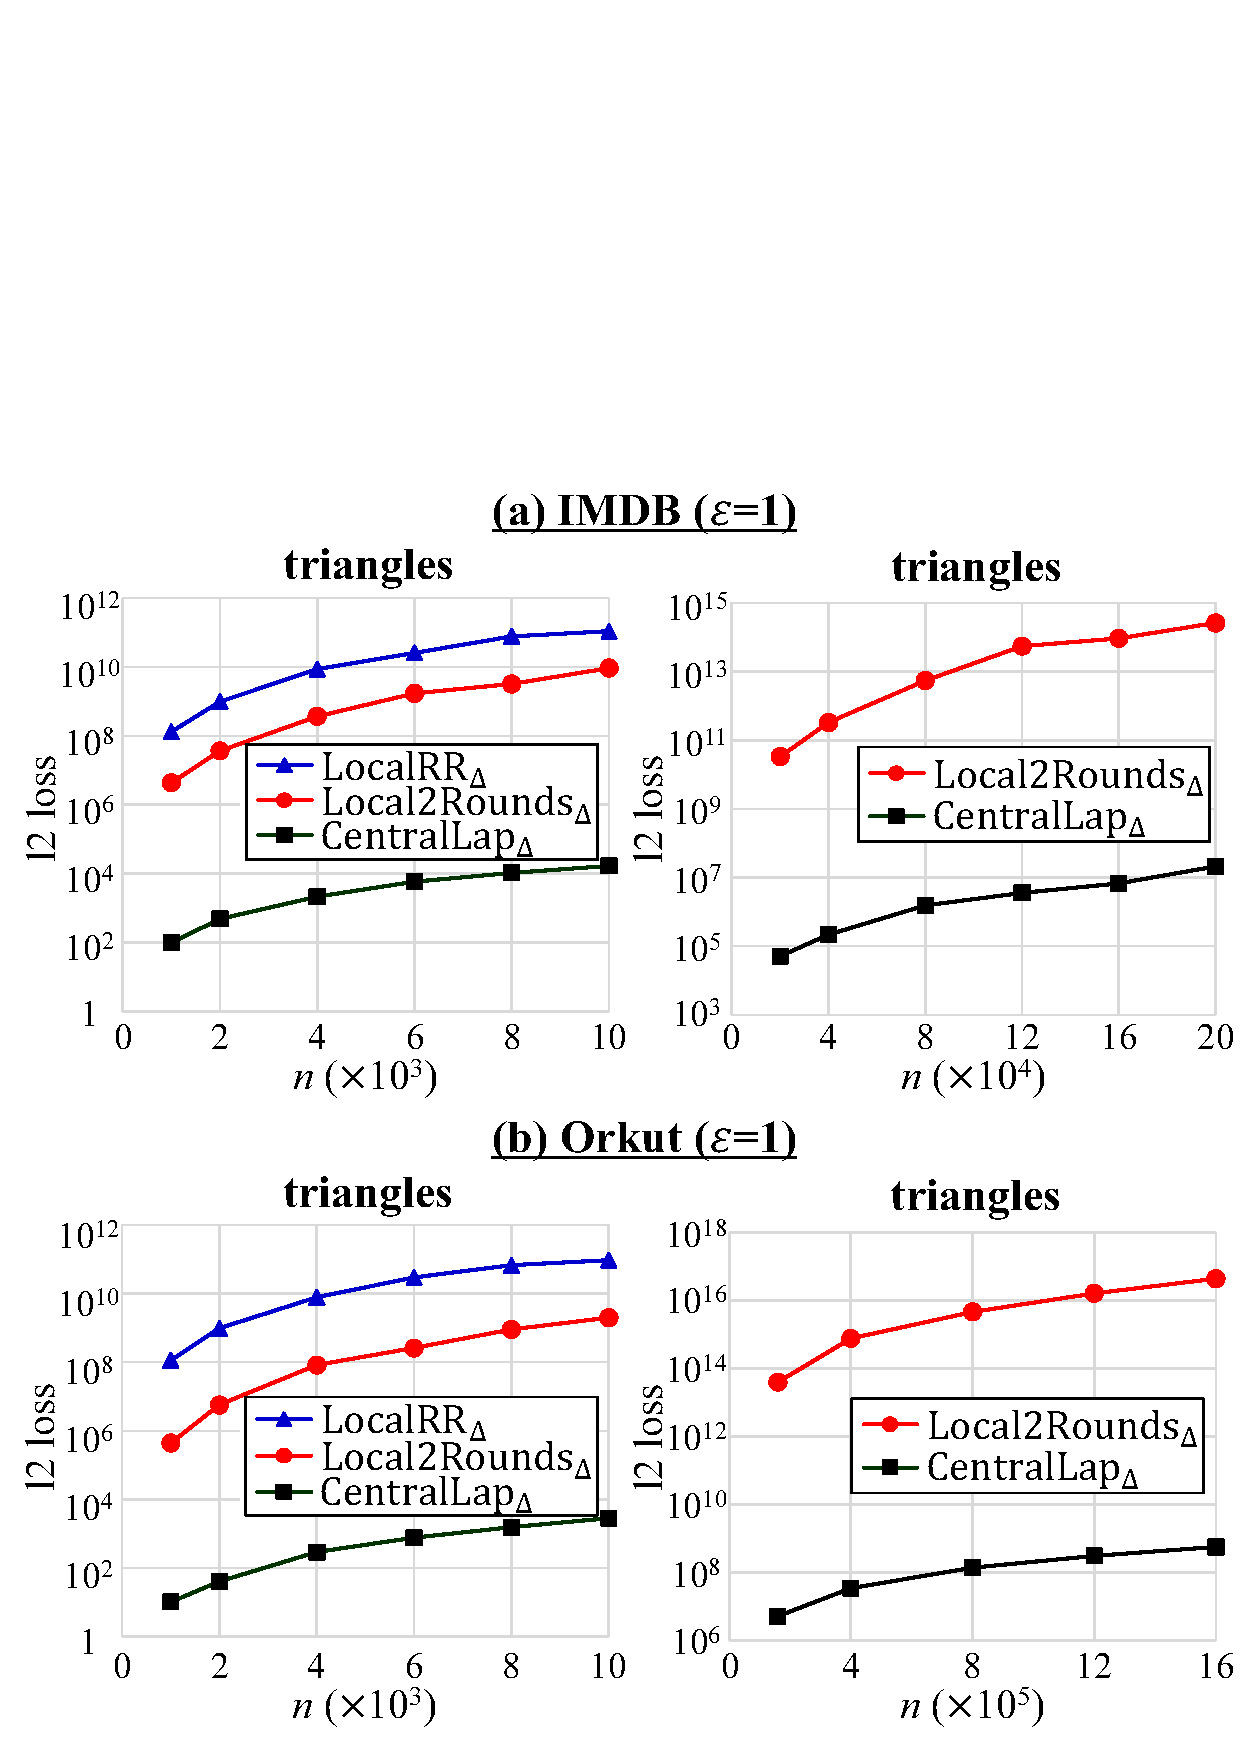
\includegraphics[width=0.99\linewidth]{fig/res1_n_l2loss_tri.pdf}

\caption[Relation between the number of users $n$ and the $l_2$ loss in triangle counts.]
{Relation between the number of users $n$ and the $l_2$ loss in triangle counts when $\epsilon = 1$ ($\epsilon_1 = \epsilon_2 = \frac{1}{2}$, $\td_{max} = d_{max}$). 
Here we do not evaluate \alg{LocalRR$_\triangle$} when $n > 10000$, because it is inefficient (see Section~\ref{chap1-sub:two_rounds} ``Time complexity'').}
\label{chap1-fig:res1_n_l2loss_tri}
\end{figure}

\begin{figure}[t]
\centering
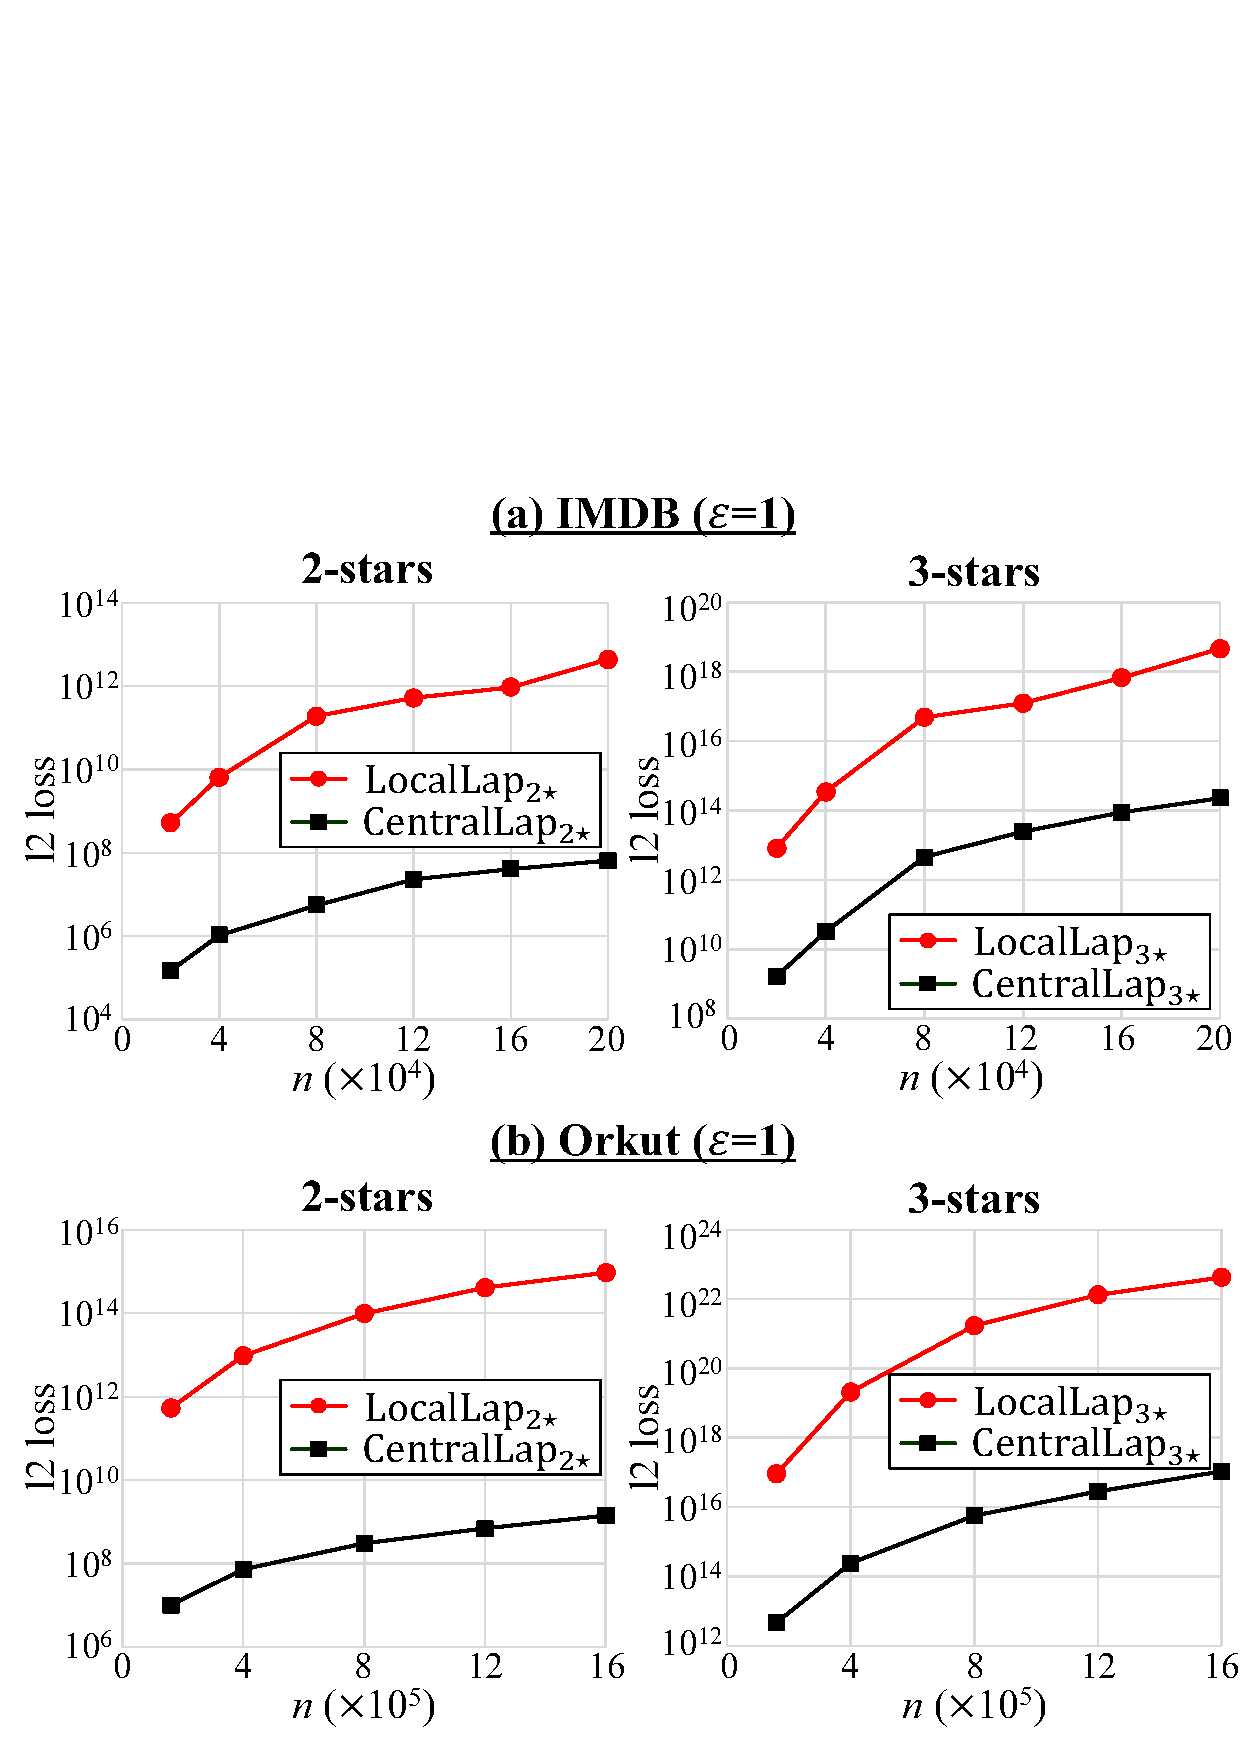
\includegraphics[width=0.99\linewidth]{fig/res1_n_l2loss_kst.pdf}

\caption[Relation between the number of users $n$ and the $l_2$ loss in $k$-star counts.]
{Relation between the number of users $n$ and the $l_2$ loss in $k$-star counts when $\epsilon=1$ ($\epsilon_1 = \epsilon_2 = \frac{1}{2}$, $\td_{max} = d_{max}$).}
\label{chap1-fig:res1_n_l2loss_kst}
\end{figure}

\subsection{Experimental Results}
\label{chap1-sub:results}
\noindent{\textbf{Relation between $n$ and the $l_2$ loss.}}~~We first evaluated the $l_2$ loss of the estimates of 
% the numbers of triangles ($f_\triangle(G)$), $2$-stars ($f_{2\star}(G)$), and $3$-stars ($f_{3\star}(G)$), 
$f_\triangle(G)$, 
% (triangle counts), 
$f_{2\star}(G)$, 
% ($2$-star counts), 
and $f_{3\star}(G)$ 
% ($3$-star counts) 
while changing the number of users $n$. 
Figures~\ref{chap1-fig:res1_n_l2loss_tri} and \ref{chap1-fig:res1_n_l2loss_kst} shows the results ($\epsilon=1$). 
Here 
% we changed $n$ from $1000$ to $200000$ in \IMDB{}, and from $1000$ to $1600000$ in \Orkut{}. 
% Note that 
we did not evaluate \alg{LocalRR$_\triangle$} when $n$ was larger than $10000$, because \alg{LocalRR$_\triangle$} was inefficient 
% (the time complexity of \alg{LocalRR$_\triangle$} is $O(n^3)$, as described in Section~\ref{chap1-sub:two_rounds}). 
(as described in Section~\ref{chap1-sub:two_rounds} ``Time complexity''). 
% In Figures~\ref{chap1-fig:res1_n_l2loss_tri} and \ref{chap1-fig:res1_n_l2loss_kst}, 
In \alg{Local2Rounds$_\triangle$}, we set $\epsilon_1 = \epsilon_2 = \frac{1}{2}$. 
% so that $\epsilon = \epsilon_1 + \epsilon_2 = 1$. 
% In \alg{Local2Rounds$_\triangle$},  \alg{CentralLap$_\triangle$}, \alg{LocalLap$_k\star$}, and \alg{CentralLap$_k\star$}, 
As for $\td_{max}$, 
we set $\td_{max} = d_{max}$ (i.e., we assumed that $d_{max}$ is publicly available and did not perform graph projection) 
% , 
because we want to examine how well our theoretical results hold in our experiments. 
% we added the Laplacian noise with the local sensitivity in \alg{Proposal}, \alg{central (Lap)}, and \alg{local (Lap)}. 
We also evaluate the effectiveness of the private calculation of $d_{max}$ at the end of Section~\ref{chap1-sub:results}. 

Figure~\ref{chap1-fig:res1_n_l2loss_tri} shows that \alg{Local2Rounds$_\triangle$} significantly outperforms \alg{LocalRR$_\triangle$}. 
% for estimating $f_\triangle(G)$. 
Specifically, the $l_2$ loss of \alg{Local2Rounds$_\triangle$} is smaller than that of \alg{LocalRR$_\triangle$} by a factor of about $10^2$. 
% and $10^2 \sim 10^3$ in \IMDB{} and \Orkut{}, respectively. 
The difference between \alg{Local2Rounds$_\triangle$} and \alg{LocalRR$_\triangle$} is larger in \Orkut{}. 
This is because \Orkut{} is more sparse, as described in Section~\ref{chap1-sub:setup}. 
For example, when $n=10000$, the maximum degree $d_{max}$ in $G$ was $73.5$ and $27.8$ on average in \IMDB{} and \Orkut{}, respectively. 
Recall that for a fixed $\epsilon$, 
the expected $l_2$ loss of \alg{Local2Rounds$_\triangle$} and \alg{LocalRR$_\triangle$} 
can be expressed as $O(nd_{max}^3)$ and $O(n^4)$, respectively. 
Thus \alg{Local2Rounds$_\triangle$} significantly outperforms \alg{LocalRR$_\triangle$}, especially in sparse graphs. 
% datasets. 

% Figures~\ref{chap1-fig:res1_n_l2loss_tri} and \ref{chap1-fig:res1_n_l2loss_kst} show that \alg{central (Lap)} provides the best performance, which is consistent with our theoretical results; i.e., 

Figures~\ref{chap1-fig:res1_n_l2loss_tri} and \ref{chap1-fig:res1_n_l2loss_kst} show that the $l_2$ loss is roughly consistent with 
our upper-bounds in terms of $n$. 
Specifically, 
\alg{LocalRR$_\triangle$}, 
\alg{Local2Rounds$_\triangle$},  \alg{CentralLap$_\triangle$}, 
\alg{LocalLap$_{k\star}$}, and 
\alg{CentralLap$_{k\star}$} achieve 
the expected $l_2$ loss of $O(n^4)$, $O(nd_{max}^3)$, $O(d_{max}^2)$, $O(nd_{max}^{2k-2})$, and $O(d_{max}^{2k-2})$, respectively. 
Here note that 
% the maximum degree $d_{max}$ increases roughly in proportion to $n$ (though $d_{max}$ is much smaller than $n$), 
each user's degree increases roughly in proportion to $n$ (though the degree is much smaller than $n$), 
as we randomly select $n$ users from the whole graph $G^*$. Assuming that $d_{max} = O(n)$,  Figures~\ref{chap1-fig:res1_n_l2loss_tri} and \ref{chap1-fig:res1_n_l2loss_kst} are roughly consistent with the upper-bounds. 
The figures also show the limitations of the local model in terms of the utility when compared to the centralized model.

% when we increase $n$ by a factor of $10$, 
% the $l_2$ loss in triangle counts increases by a factor of about $10^4$, $10^4$, $10^2$ in \alg{LocalRR$_\triangle$}, \alg{Local2Rounds$_\triangle$}, and \alg{central (Lap)}, respectively. 
% Therefore, the experimental results are roughly consistent with our theoretical results that the expected $l_2$ loss of \alg{LocalRR$_\triangle$}, \alg{Local2Rounds$_\triangle$}, and \alg{CentralLap$_\triangle$} is $O(n^4)$, $O(nd_{max}^3)$, and $O(d_{max}^2)$, respectively. 
% The same applies to $k$-star counts. 

\smallskip
\noindent{\textbf{Relation between $\epsilon$ and the $l_2$ loss.}}~~Next we evaluated the $l_2$ loss 
% of the estimates of $f_\triangle(G)$ (triangle counts) and $f_{2\star}(G)$ ($2$-star counts), 
when we changed the privacy budget $\epsilon$ in edge LDP. 
Figure~\ref{chap1-fig:res2_eps_l2loss} shows the results for triangles and $2$-stars ($n=10000$). 
% (the result of $3$-stars is similar to that of $2$-stars, and therefore we omit the result of $3$-stars). 
Here we omit the result of $3$-stars because it is similar to that of $2$-stars. 
In \alg{Local2Rounds$_\triangle$}, we set $\epsilon_1 = \epsilon_2 = \frac{\epsilon}{2}$. 

Figure~\ref{chap1-fig:res2_eps_l2loss} shows that the $l_2$ loss is roughly consistent with 
% the expected $l_2$ loss in 
% our theoretical analysis 
our upper-bounds in terms of $\epsilon$. 
For example, when we decrease $\epsilon$ from $0.4$ to $0.1$, the $l_2$ loss 
% in triangle counts 
increases by a factor of about $5000$, $200$, and $16$ for both the datasets in \alg{LocalRR$_\triangle$}, \alg{Local2Rounds$_\triangle$}, and \alg{CentralLap$_\triangle$}, respectively. 
% This is 
They are 
roughly consistent with our theoretical results 
that for small $\epsilon$, the expected $l_2$ loss of \alg{LocalRR$_\triangle$}, \alg{Local2Rounds$_\triangle$}, and \alg{CentralLap$_\triangle$} is  $O(\epsilon^{-6})$\footnote{We used $e^\epsilon \approx \epsilon + 1$ to derive the upper-bound of \alg{LocalRR$_\triangle$} for small $\epsilon$.}, $O(\epsilon^{-4})$, and $O(\epsilon^{-2})$, respectively. 
% The same applies to large $\epsilon$ (e.g., $\epsilon = 1$ or $2$). 

\begin{figure}[t]
\centering
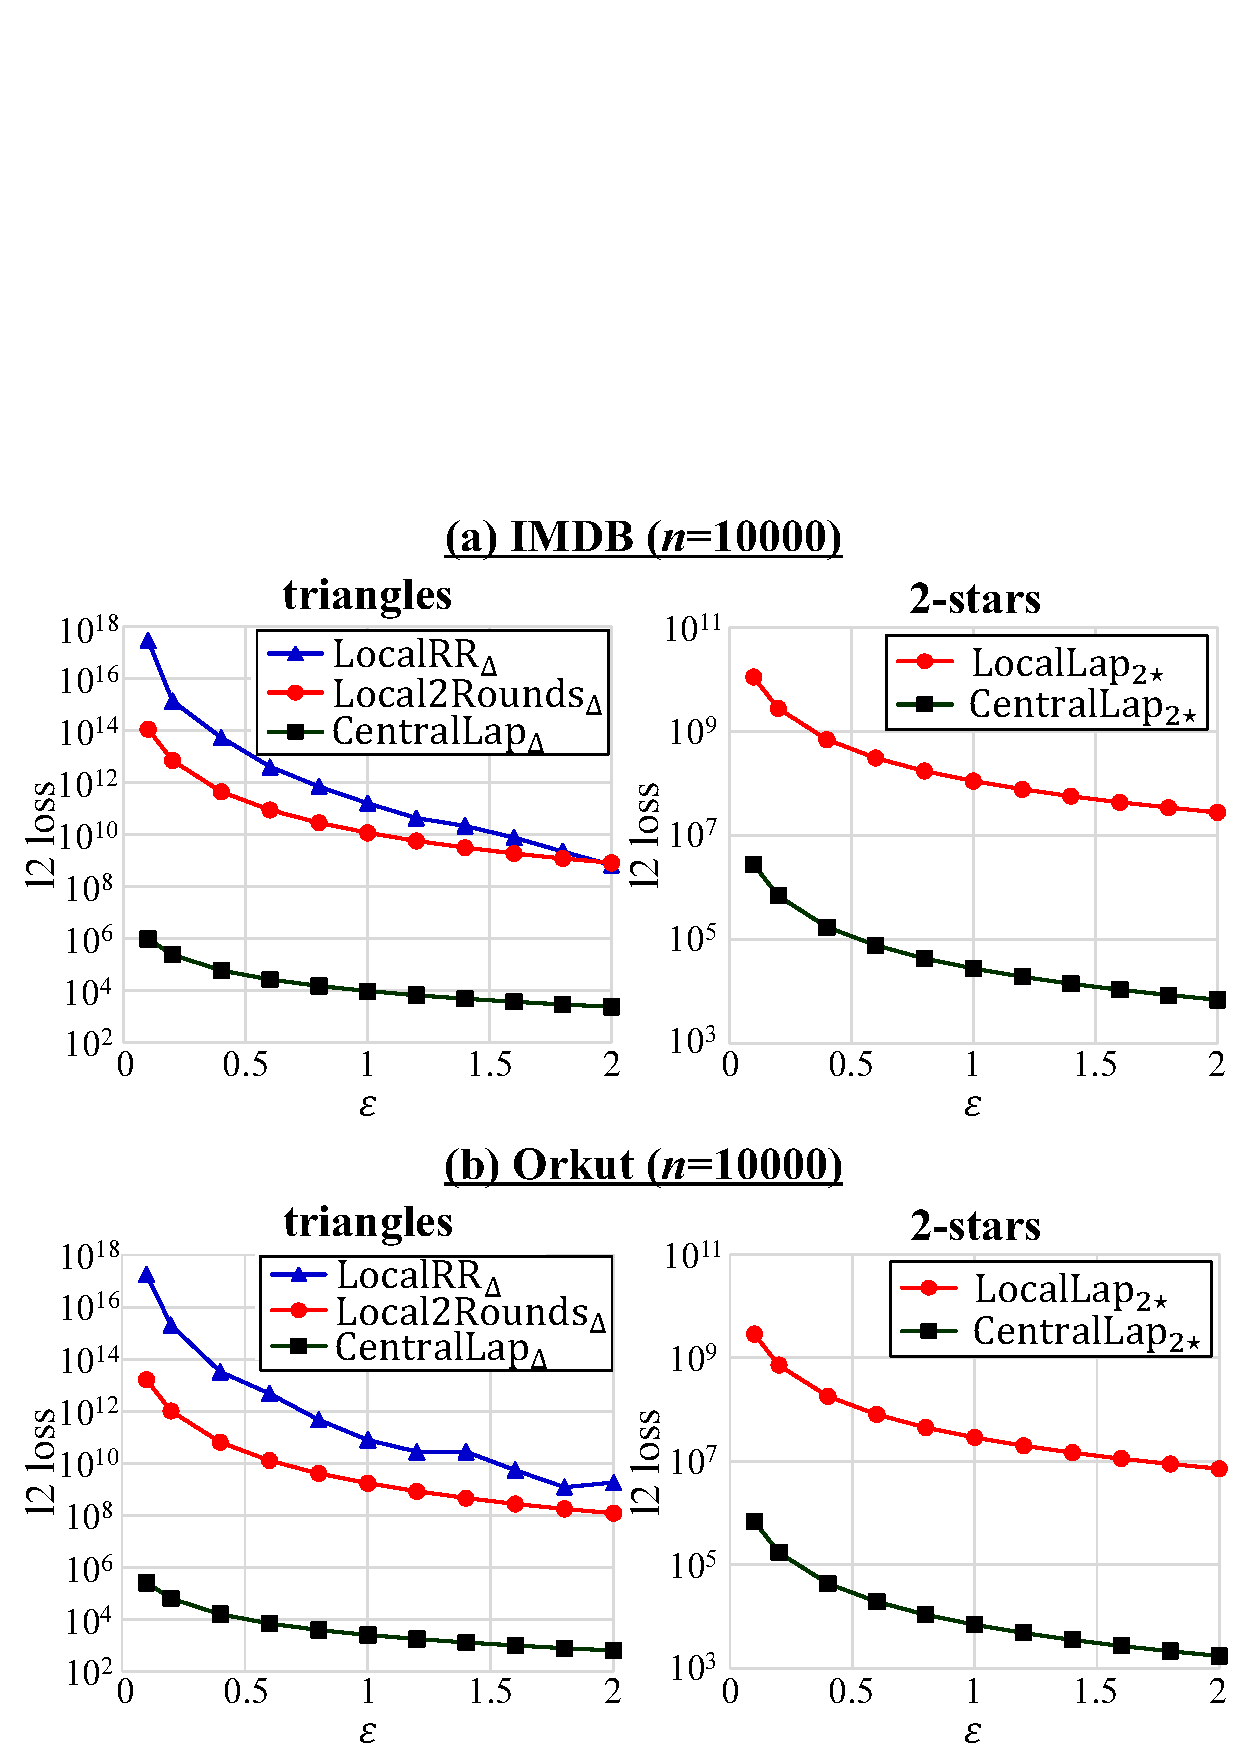
\includegraphics[width=0.99\linewidth]{fig/res2_eps_l2loss.pdf}

\caption[Relation between $\epsilon$ in edge LDP and the $l_2$ loss.]
{Relation between $\epsilon$ in edge LDP and the $l_2$ loss when $n=10000$ ($\epsilon_1 = \epsilon_2 = \frac{\epsilon}{2}$, $\td_{max} = d_{max}$).}
\label{chap1-fig:res2_eps_l2loss}
\end{figure}

\begin{figure}[t]
\centering
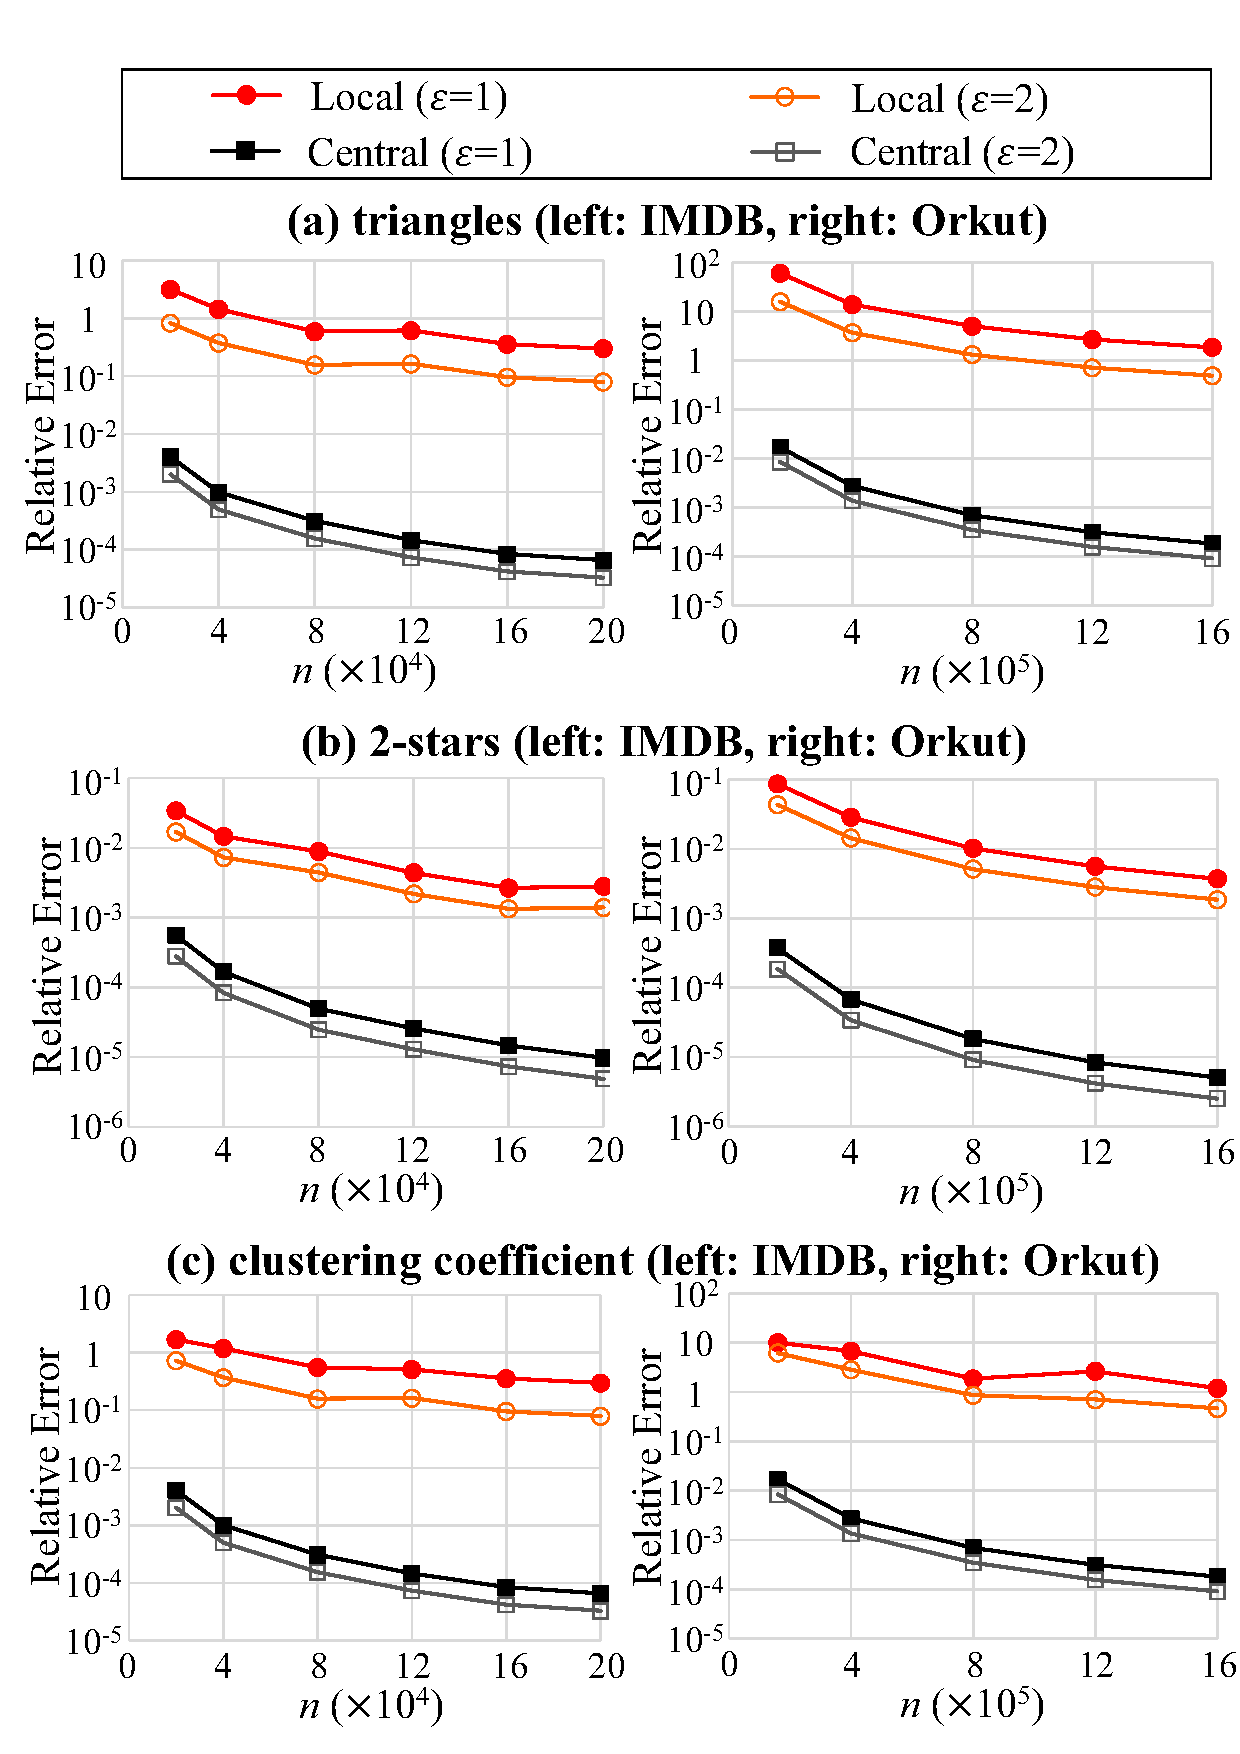
\includegraphics[width=0.99\linewidth]{fig/res3_n_relerr.pdf}

\caption[Relation between $n$ and the relative error.]{Relation between 
$n$ and the relative error. In the local model, we used \alg{Local2Rounds$_\triangle$} ($\epsilon = 1$ or $2$) and \alg{LocalLap$_k\star$} ($\epsilon = 1$ or $2$) for estimating triangle counts $f_\triangle(G)$ and $k$-star counts $f_{k\star}(G)$, respectively ($\td_{max} = d_{max}$).}
\label{chap1-fig:res3_n_relerr}
\end{figure}

Figure~\ref{chap1-fig:res2_eps_l2loss} also shows that 
\alg{Local2Rounds$_\triangle$} significantly outperforms \alg{LocalRR$_\triangle$} especially when $\epsilon$ is small, which is also consistent with our theoretical results. 
Conversely, the difference between \alg{LocalRR$_\triangle$} and \alg{Local2Rounds$_\triangle$} is small when $\epsilon$ is large. 
This is because when $\epsilon$ is large, the RR outputs the true value with high probability. 
For example, when 
% $\epsilon \geq 3$, 
$\epsilon \geq 5$, 
the RR outputs the true value with 
% $\frac{e^\epsilon}{e^\epsilon+1} > 0.95$. 
$\frac{e^\epsilon}{e^\epsilon+1} > 0.993$. 
% We also confirmed that when $\epsilon \geq 3$, the $l_2$ loss of \alg{LocalRR$_\triangle$} is smaller than \alg{Local2Rounds$_\triangle$} in both the datasets. 
However, \alg{LocalRR$_\triangle$} with 
% $\epsilon \geq 3$ 
such a large value of $\epsilon$ 
does not guarantee strong privacy, because it outputs the true value in most cases. 
% with more than $95\%$. 
\alg{Local2Rounds$_\triangle$} significantly outperforms \alg{LocalRR$_\triangle$} 
% for a reasonable range of $\epsilon$. 
when we want to estimate $f_\triangle(G)$ or $f_{k\star}(G)$ 
with a strong privacy guarantee; e.g., $\epsilon \leq 1$ \cite{DP_Li}. 

\smallskip
\noindent{\textbf{Relative error.}}~~As the number of users $n$ increases, the numbers of triangles $f_\triangle(G)$ and $k$-stars $f_{k\star}(G)$ increase. 
% , and this 
This causes the increase of the $l_2$ loss. 
Therefore, we also evaluated the relative error, as described in Section~\ref{chap1-sub:graph_statistics}. 

Figure~\ref{chap1-fig:res3_n_relerr} shows the relation between $n$ and the relative error 
(we omit the result of $3$-stars because it is similar to that of $2$-stars). 
In the local model, we used \alg{Local2Rounds$_\triangle$} and \alg{LocalLap$_k\star$} for estimating 
% triangle counts 
$f_\triangle(G)$ 
and 
% $k$-star counts, 
$f_{k\star}(G)$, 
respectively 
(we did not use \alg{Local2RR$_\triangle$}, because it is both inaccurate and inefficient). 
For both algorithms, we set $\epsilon = 1$ or $2$ 
($\epsilon_1 = \epsilon_2 = \frac{\epsilon}{2}$ in \alg{Local2Rounds$_\triangle$}) and $\td_{max} = d_{max}$. 
Then we estimated the clustering coefficient as: $\frac{3\hf_{\triangle}(G, \epsilon_1, \epsilon_2, d_{max})}{\hf_{k\star}(G, \epsilon, d_{max})}$, where 
$\hf_{\triangle}(G, \epsilon_1, \epsilon_2, d_{max})$ and 
$\hf_{k\star}(G, \epsilon, d_{max})$ are the estimates of $f_\triangle(G)$ and $f_{k\star}(G)$, respectively. 
If the estimate of the clustering coefficient is smaller than $0$ (resp.~larger than $1$), we set the estimate to $0$ (resp.~$1$) because the clustering coefficient is always between $0$ and $1$. 
In the centralized model, we used \alg{CentralLap$_\triangle$} and \alg{CentralLap$_k\star$} ($\epsilon=1$ or $2$, $\td_{max} = d_{max}$) and calculated the clustering coefficient in the same way. 

Figure~\ref{chap1-fig:res3_n_relerr} shows that for all cases, the relative error decreases with increase in $n$. 
This is because both $f_\triangle(G)$ and $f_{k\star}(G)$ significantly increase with increase in $n$. 
Specifically, let $f_{\triangle,v_i}(G) \in \nnints$ the number of triangles that involve user $v_i$, and $f_{k\star,v_i}(G) \in \nnints$ be the number of $k$-stars of which user $v_i$ is a center. 
Then $f_\triangle(G) = \frac{1}{3}\sum_{i=1}^n f_{\triangle,v_i}(G)$ and $f_{k\star,v_i}(G) = \sum_{i=1}^n f_{k\star,v_i}(G)$. 
Since both $f_{\triangle,v_i}(G)$ and $f_{k\star,v_i}(G)$ increase with increase in $n$, both $f_\triangle(G)$ and $f_{k\star}(G)$ increase \textit{at least} in proportion to $n$. 
Thus $f_\triangle(G)^2 \geq \Omega(n^2)$ and $f_{k\star}(G)^2 \geq \Omega(n^2)$. 
In contrast, \alg{Local2Rounds$_\triangle$}, \alg{LocalLap$_k\star$}, \alg{CentralLap$_\triangle$}, and \alg{CentralLap$_k\star$} achieve the expected $l_2$ loss of $O(n)$, $O(n)$, $O(1)$, and $O(1)$, respectively (when we ignore $d_{max}$ and $\epsilon$), all of which are smaller than $O(n^2)$. 
% the value $\frac{|\hf(G) - f(G)|}{|f(G)|}$ decreases with increase in $n$. 
% This explains the reason that 
Therefore, the relative error decreases with increase in $n$. 

This result demonstrates that we can accurately estimate graph statistics for large $n$ in the local model. 
In particular, the relative error is smaller in \IMDB{} 
% , 
because \IMDB{} is denser and includes a larger number of triangles and $k$-stars; i.e., the denominator of the relative error is large. 
For example, when $n=200000$ and $\epsilon=1$, the relative error is 
% $0.19$, 
$0.30$ and 
$0.0028$ 
% , and $0.015$ 
for triangles and $2$-stars, 
% , and $3$-stars, 
respectively. 
Note that the clustering coefficient requires $2\epsilon$ 
% , 
because we need to estimate both $f_\triangle(G)$ and $f_{k\star}(G)$. 
Yet, we can still accurately calculate the clustering coefficient with a moderate privacy budget; 
% $\epsilon$; 
e.g., the relative error of the clustering coefficient is 
%$0.19$ 
$0.30$ 
when the privacy budget is $2$ (i.e., $\epsilon = 1$).
If $n$ is larger, then $\epsilon$ would be smaller at the same value of the relative error. 

\begin{figure}[t]
\centering
% 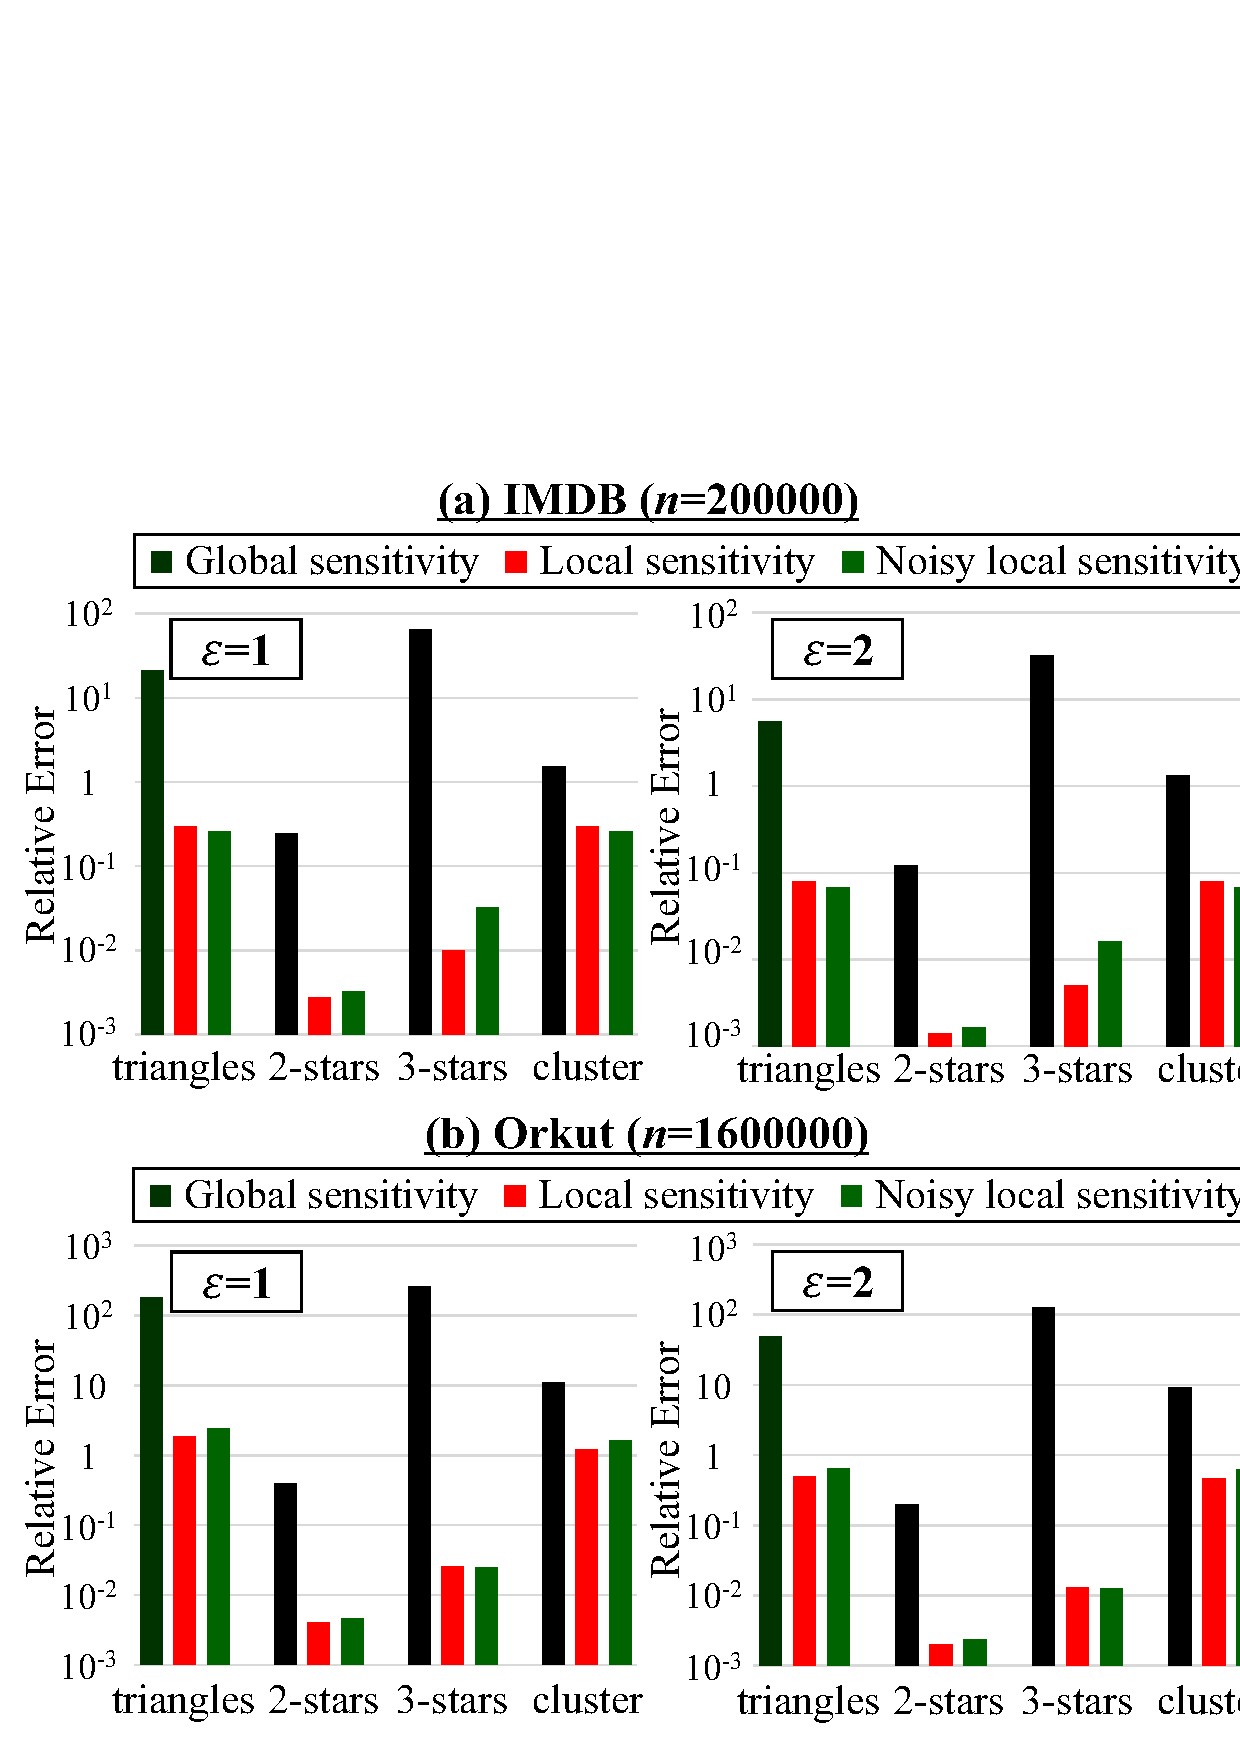
\includegraphics[width=0.99\linewidth]{fig/res4_noisy_local.pdf}
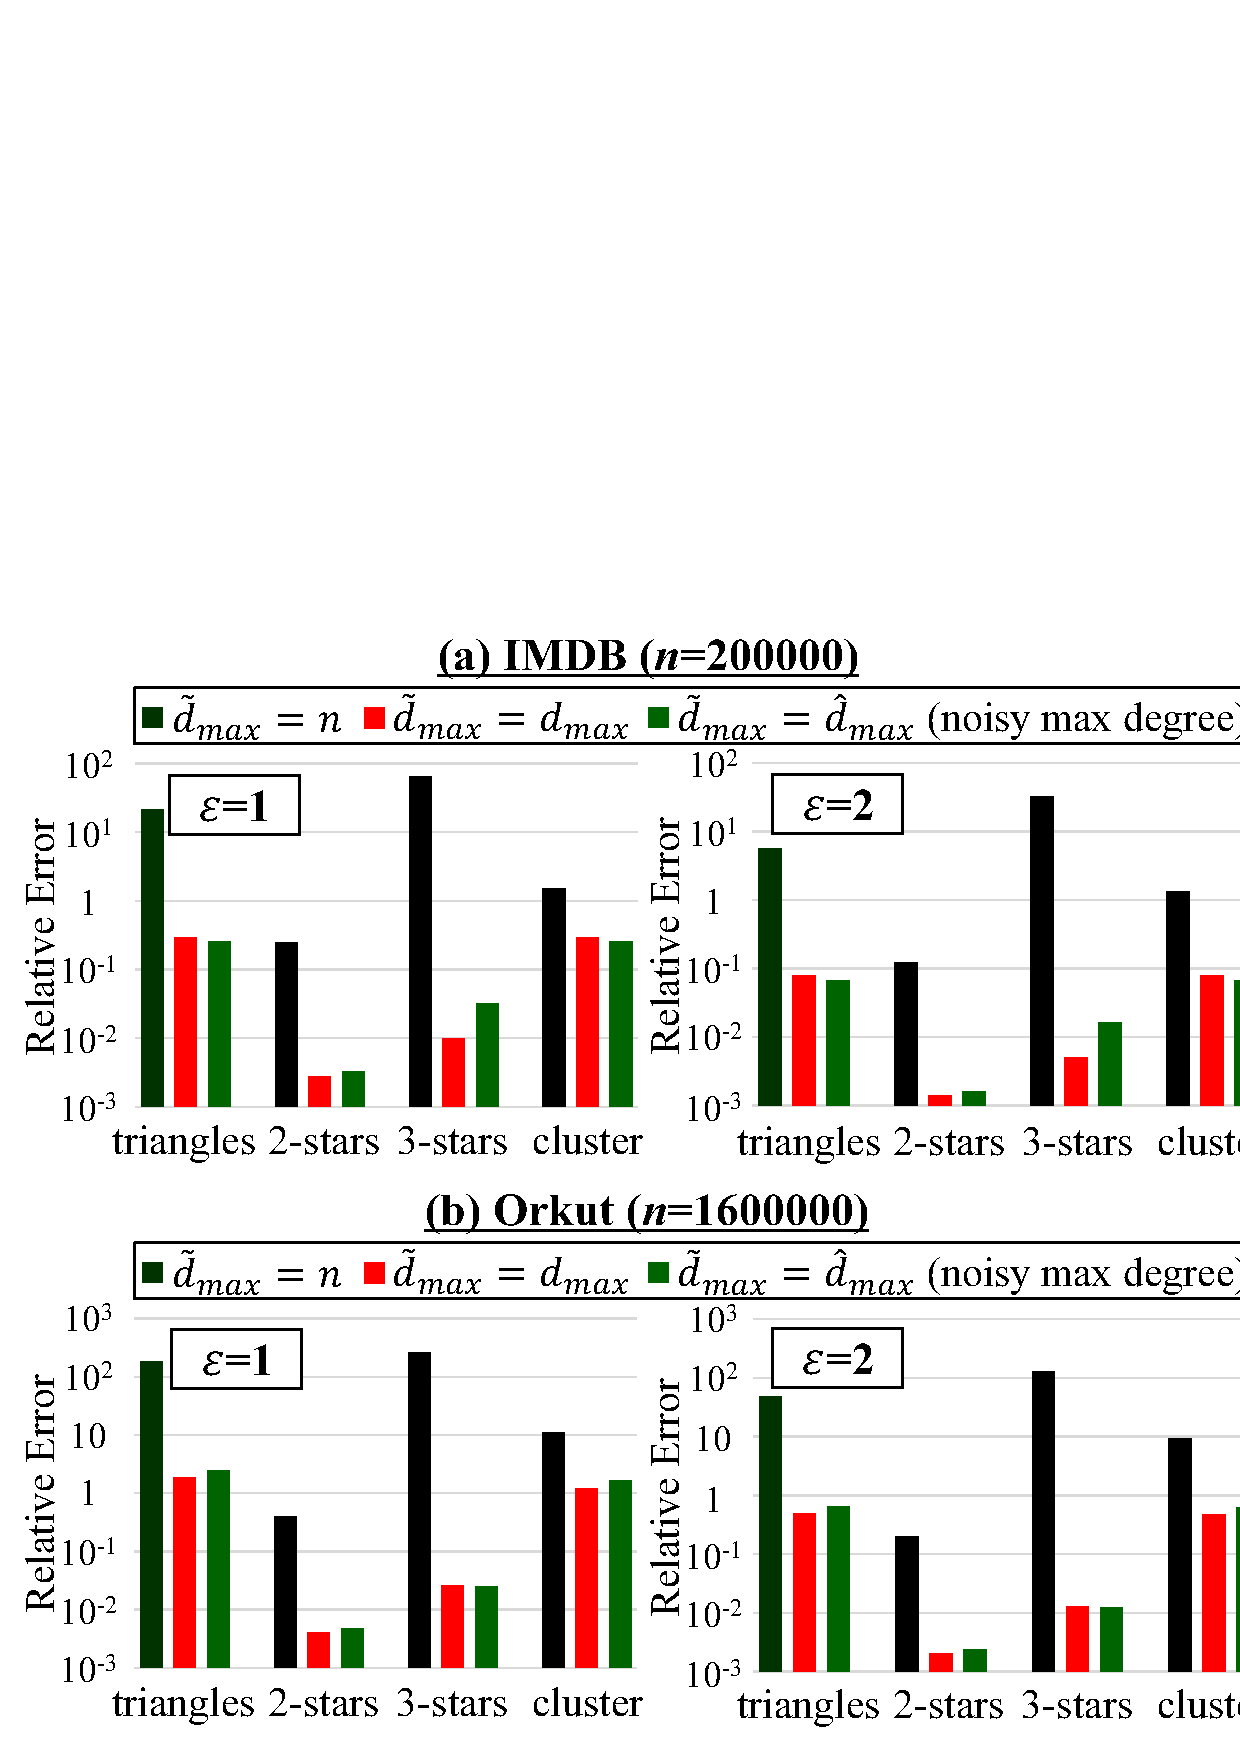
\includegraphics[width=0.99\linewidth]{fig/res4_noisy_max.pdf}

\caption[Relative error when $\td_{max}$ equals \#users, max degree, or noisy max degree.]
{Relative error when $\td_{max} = n$ (\#users), $d_{max}$ (max degree), or $\hd_{max}$ (noisy max degree). 
We used \alg{Local2Rounds$_\triangle$} ($\epsilon = 1$ or $2$) and \alg{LocalLap$_k\star$} ($\epsilon = 1$ or $2$) for estimating triangle counts $f_\triangle(G)$ and $k$-star counts $f_{k\star}(G)$, respectively. 
}
\label{chap1-fig:res4_noisy_local}
\end{figure}

\smallskip
\noindent{\textbf{Private calculation of $d_{max}$.}}~~We have so far assumed that $\td_{max} = d_{max}$ (i.e., $d_{max}$ is publicly available) in our experiments. 
% However, it is difficult for the users and the data collector to know the exact value of $d_{max}$ in advance. 
% Therefore, we 
We 
finally evaluate the methods to privately calculate $d_{max}$ with $\epsilon_0$-edge LDP 
% , which are 
(described in Sections~\ref{chap1-sub:non-interactive_k_stars} and \ref{chap1-sub:two_rounds}). 
% show that even if we privately calculate $d_{max}$ with edge LDP, we can accurately estimate graph statistics in the local model. 

Specifically, we used \alg{Local2Rounds$_\triangle$} and \alg{LocalLap$_k\star$} for estimating $f_\triangle(G)$ and $f_{k\star}(G)$, respectively, and evaluated the following three methods for setting $\td_{max}$: 
% the sensitivity: 
% \begin{enumerate}
%     \item Set $\td_{max} = n$. We call this method the \textit{global sensitivity method} because it results in adding the Laplacian noise with the global sensitivity in Definition~\ref{chap1-def:global_sen}.
%     \item Set $\td_{max} = d_{max}$. We call this method the \textit{local sensitivity method} because it results in adding the Laplacian noise with the local sensitivity. 
% \end{enumerate}
(i) 
% set 
$\td_{max} = n$; 
(ii) 
% set 
$\td_{max} = d_{max}$; 
(iii) 
% set 
$\td_{max} = \hd_{max}$, where $\hd_{max}$ is the private estimate of $d_{max}$ 
% (i.e., 
(noisy max degree) in Sections~\ref{chap1-sub:non-interactive_k_stars} and \ref{chap1-sub:two_rounds}. 
% Note that the first (resp.~second) method results in adding the Laplacian noise with the global (resp.~local) sensitivity without using graph projection. 
% Therefore, we refer to the first method (i) as the \textit{global sensitivity method}, the second method (ii) as the \textit{local sensitivity method}, and the third method (iii) as the \textit{noisy local sensitivity method}. 

We set $n=200000$ in \IMDB{} and $n=1600000$ in \Orkut{}. 
Regarding the total privacy budget $\epsilon$ in edge LDP for estimating $f_\triangle(G)$ or $f_{k\star}(G)$, we set $\epsilon=1$ or $2$. 
We used $\frac{\epsilon}{10}$ for privately calculating $d_{max}$ (i.e., $\epsilon_0 = \frac{\epsilon}{10}$), and the remaining privacy budget $\frac{9\epsilon}{10}$ as input to \alg{Local2Rounds$_\triangle$} or \alg{LocalLap$_k\star$}. 
% estimating $f_\triangle(G)$ or $f_{k\star}(G)$. 
In \alg{Local2Rounds$_\triangle$}, we set $\epsilon_1 = \epsilon_2$; i.e., we set $(\epsilon_0, \epsilon_1, \epsilon_2) = (0.1, 0.45, 0.45)$ or $(0.2, 0.9, 0.9)$. 
% For example, \alg{Local2Rounds$_\triangle$} with $(\epsilon_0, \epsilon_1, \epsilon_2) = (0.1, 0.45, 0.45)$ provides $1$-edge LDP and $1.1$-entire edge LDP (see Section~\ref{chap1-sub:two_rounds}). 
Then we estimated the clustering coefficient in the same way as Figure~\ref{chap1-fig:res3_n_relerr}. 

Figure~\ref{chap1-fig:res4_noisy_local} shows the results. 
Figure~\ref{chap1-fig:res4_noisy_local} shows that 
% the noisy local sensitivity method 
the algorithms with $\td_{max} = \hd_{max}$ (noisy max degree) 
achieves the relative error close to (sometimes almost the same as) 
% the local sensitivity method, 
the algorithms with $\td_{max} = d_{max}$ 
and significantly outperforms 
% the global sensitivity method. 
the algorithms with $\td_{max} = n$. 
This means that we can privately estimate $d_{max}$ without a significant loss of utility. 
% Recall that the private calculation of $d_{max}$ does not increase the number of rounds in \alg{Local2Rounds$_\triangle$}. 
% Therefore, we can privately estimate $d_{max}$ and then accurately estimate all the graph statistics (i.e., triangles, $k$-stars, and the clustering coefficient) within two rounds.

\smallskip
\noindent{\textbf{Summary of results.}}~~In summary, 
% our experimental results were roughly consistent with our theoretical results. 
our experimental results showed that the estimation error of triangle counts is significantly reduced by introducing the interaction between users and a data collector. 
The results also showed that 
% we can accurately estimate graph statistics in the local model. 
% In particular, 
we can achieve small relative errors 
(much smaller than 1) for subgraph counts 
% for a large number of users $n$ 
with privacy budget $\epsilon=1$ or $2$ in edge LDP. 
% The results also showed that we can privately estimate the maximum degree $d_{max}$, which is required in both \alg{Local2Rounds$_\triangle$} and \alg{LocalLap$_k\star$}, without a significant loss of utility. 

As described in Section~\ref{chap1-sec:intro}, non-private 
% triangle or $k$-star 
subgraph 
counts may reveal some friendship information, and a central server may face data breaches. 
Our LDP algorithms are highly beneficial because they enable us to analyze the connection patterns in a graph 
(i.e., subgraph counts) 
or to understand how likely two friends of an individual will also be a friend 
% (which is useful for friend suggestion) 
(i.e., clustering coefficient) 
while strongly protecting individual privacy.


\section{Conclusions}
\label{sec:conclusions}
% In this paper, we proposed
% locally private
We proposed
triangle counting algorithms under edge LDP with a small estimation error and small communication cost.
We showed that
% the estimation error can be significantly reduced by our 4-cycle trick and double clipping, and that
our entire algorithms with the 4-cycle trick and double clipping
can dramatically reduce the download cost
% when compared with
of
\cite{Imola_USENIX21}
% (e.g., from $400$ Gbits to $100$ Mbits).
(e.g., from 6 hours to 8 seconds or less). 
% when $20$ Mbps).
% In \cite{Imola_USENIX21},

% In this paper,
We assumed that each user $v_i$ honestly inputs her neighbor list $\bma_i$, as in most previous work on LDP.
However, recent studies \cite{Cao_USENIX21,Cheu_SP21} show that the estimate in LDP can be skewed by data poisoning attacks.
% with a number of malicious accounts.
As future work, we would like to analyze the impact of data poisoning on our algorithms and develop defenses (e.g., detection) against it.


% %-------------------------------------------------------------------------------
\section*{Acknowledgments}
Kamalika Chaudhuri and Jacob Imola would like to thank ONR under N00014-20-1-2334 and UC Lab Fees under LFR 18-548554  for research support.
Takao Murakami was supported in part by JSPS KAKENHI JP19H04113.

%-------------------------------------------------------------------------------

%-------------------------------------------------------------------------------
\bibliographystyle{plain}
%\bibliographystyle{abbrv}
% \bibliography{main}
% \bibliography{main_short}
\bibliography{main_sshort}

\graphicspath{{./chapters/chapter2/}}
\chapter{ }

\section{Basic Notations}
\label{chap2-sec:notations_subgraphs}

Table~\ref{chap2-tab:notations} shows the basic notations used in this paper.
% We also show subgraphs that appear in our theoretical analysis (Theorem~\ref{chap2-thm:l2loss_algorithms}) in Figure~\ref{chap2-fig:subgraphs}.

\begin{table}[t]
\caption{Basic notations.}
\centering
\hbox to\hsize{\hfil
\begin{tabular}{l|l}
\hline
Symbol		&	Description\\
\hline
% $n$         &	    Number of users.\\
$G=(V,E)$   &	    Graph with $n$ users $V$ and edges $E$.\\
$v_i$       &       $i$-th user in $V$ (i.e., $V=\{v_1,\ldots,v_n\}$).\\
$d_{max}$   &       Maximum degree of $G$.\\
$\calG$     &       Set of possible graphs with $n$ users.\\
$f_\triangle(G)$   &  Triangle count in $G$.\\
$\bmA=(a_{i,j})$	    &		Adjacency matrix.\\
$\bma_i$	&		Neighbor list of $v_i$ (i.e., $i$-th row of $\bmA$).\\
% $\calR_i$     &       Randomized mechanism of $v_i$.\\
$\calR_i$     &       Local randomizer of $v_i$.\\
$M_i$     &       Message sent from the server to user $v_i$.\\
% $\mu_F$     &       ARR parameter $\mu$ in \AlgOne{}.\\
% $\mu_O$     &       ARR parameter $\mu$ in \AlgTwo{}.\\
% $\mu_T$     &       ARR parameter $\mu$ in \AlgThree{}.\\
$\mu$     &       Parameter in the ARR.\\
$\mu^*$     &   $=\mu, \mu^2, \mu^3$ in \AlgOne{}, \AlgTwo{}, \\
    &   and \AlgThree{}, respectively.\\
$\td_i$     &   Noisy degree of user $v_i$.\\
$\kappa_i$ &   Clipping threshold of user $v_i$.\\
% $\lambda_i$ &   Clipping coefficient of user $v_i$.\\
$\epsilon_0$     &       Privacy budget for edge clipping.\\
$\epsilon_1$     &       Privacy budget for the ARR.\\
$\epsilon_2$     &       Privacy budget for the Laplacian noise.\\
$\epsilon$     &       Total privacy budget.\\
\hline
\end{tabular}
\hfil}
\label{chap2-tab:notations}
\end{table}

\section{Comparison with One-Round Algorithms}
\label{chap2-sec:one-round}
% Some studies \cite{Imola_USENIX21,Ye_ICDE20,Ye_TKDE21} propose one-round triangle counting algorithms.

Below we show that one-round triangle counting algorithms suffer from a prohibitively large estimation error.

First, we note that all of the existing one-round triangle algorithms in \cite{Imola_USENIX21,Ye_ICDE20,Ye_TKDE21} are inefficient and \textit{cannot be directly applied to a large-scale graph} such as \GPlus{} and \IMDB{} in Section~\ref{chap2-sec:experiments}.
Specifically, in their algorithms, each user $v_i$ applies Warner's RR to each bit of her neighbor list $\bma_i$ and sends the noisy neighbor list to the server.
Then the server counts the number of noisy triangles, each of which has three noisy edges,
% from the noisy graph $G'$,
and estimates $f_\triangle(G)$ based on the noisy triangle count. 
The noisy graph $G'$ in the server is dense, and there are $O(n^3)$ noisy triangles in $G'$. 
Thus, the time complexity of the existing one-round algorithms \cite{Imola_USENIX21,Ye_ICDE20,Ye_TKDE21} is $O(n^3)$.
It is also reported in \cite{Imola_USENIX21} that when $n=10^6$, the one-round algorithms  would require about $35$ years even using a supercomputer, due to the enormous number of noisy triangles.

Therefore, we evaluated the existing one-round algorithms by taking the following two steps.
First, we evaluate all the existing algorithms in \cite{Imola_USENIX21,Ye_ICDE20,Ye_TKDE21} using small graph datasets ($n=10000$) and show that the algorithm in \cite{Imola_USENIX21} achieves the lowest estimation error.
Second, we improve the time complexity of the algorithm in \cite{Imola_USENIX21} using the ARR (i.e., edge sampling after Warner's RR) and compare it with our two-rounds algorithms using large graph datasets in Section~\ref{chap2-sec:experiments}.

\smallskip
\noindent{\textbf{Small Datasets.}}~~We first evaluated the existing algorithms in \cite{Imola_USENIX21,Ye_ICDE20,Ye_TKDE21} using small datasets.
For both \GPlus{} and \IMDB{} in Section~\ref{chap2-sec:experiments}, we first randomly selected $n=10000$ users from all users and extracted a graph with $n$ users.
Then we evaluated the relative error of the following three algorithms:
(i) \textsf{RR (biased)} \cite{Imola_USENIX21,Ye_ICDE20},
(ii) \textsf{RR (bias-reduced)} \cite{Ye_TKDE21}, and
(iii) \textsf{RR (unbiased)} \cite{Imola_USENIX21}.
All of them provide $\epsilon$-edge LDP.

% The first algorithm
\textsf{RR (biased)} simply uses the number of noisy triangles in the noisy graph $G'$ obtained by Warner's RR
% each of which has three edges
as an estimate of $f_\triangle(G)$.
Clearly, it suffers from a very large bias, as $G'$ is dense.
% The second algorithm
\textsf{RR (bias-reduced)} reduces
% the bias of \textsf{RR (biased)}
this bias
by using a noisy degree sent by each user.
However, it introduces some approximation to estimate $f_\triangle(G)$, and consequently, it is not clear whether the estimate is unbiased.
We used the mean of the noisy degrees as a representative degree to obtain the optimal privacy budget allocation (see \cite{Ye_TKDE21} for details).
% The third algorithm
\textsf{RR (unbiased)} calculates an unbiased estimate of $f_\triangle(G)$ via empirical estimation. It is proved that the estimate is unbiased \cite{Imola_USENIX21}.

In all of the three algorithms, each user $v_i$ obfuscates bits for smaller user IDs in her neighbor list $\bma_i$. 
% (i.e., the lower triangular part of $\bmA$) 
% to avoid the doubling issue in Section~\ref{chap2-sub:LDP}.
We averaged the relative error over $10$ runs.

\begin{figure}[t]
  \centering
  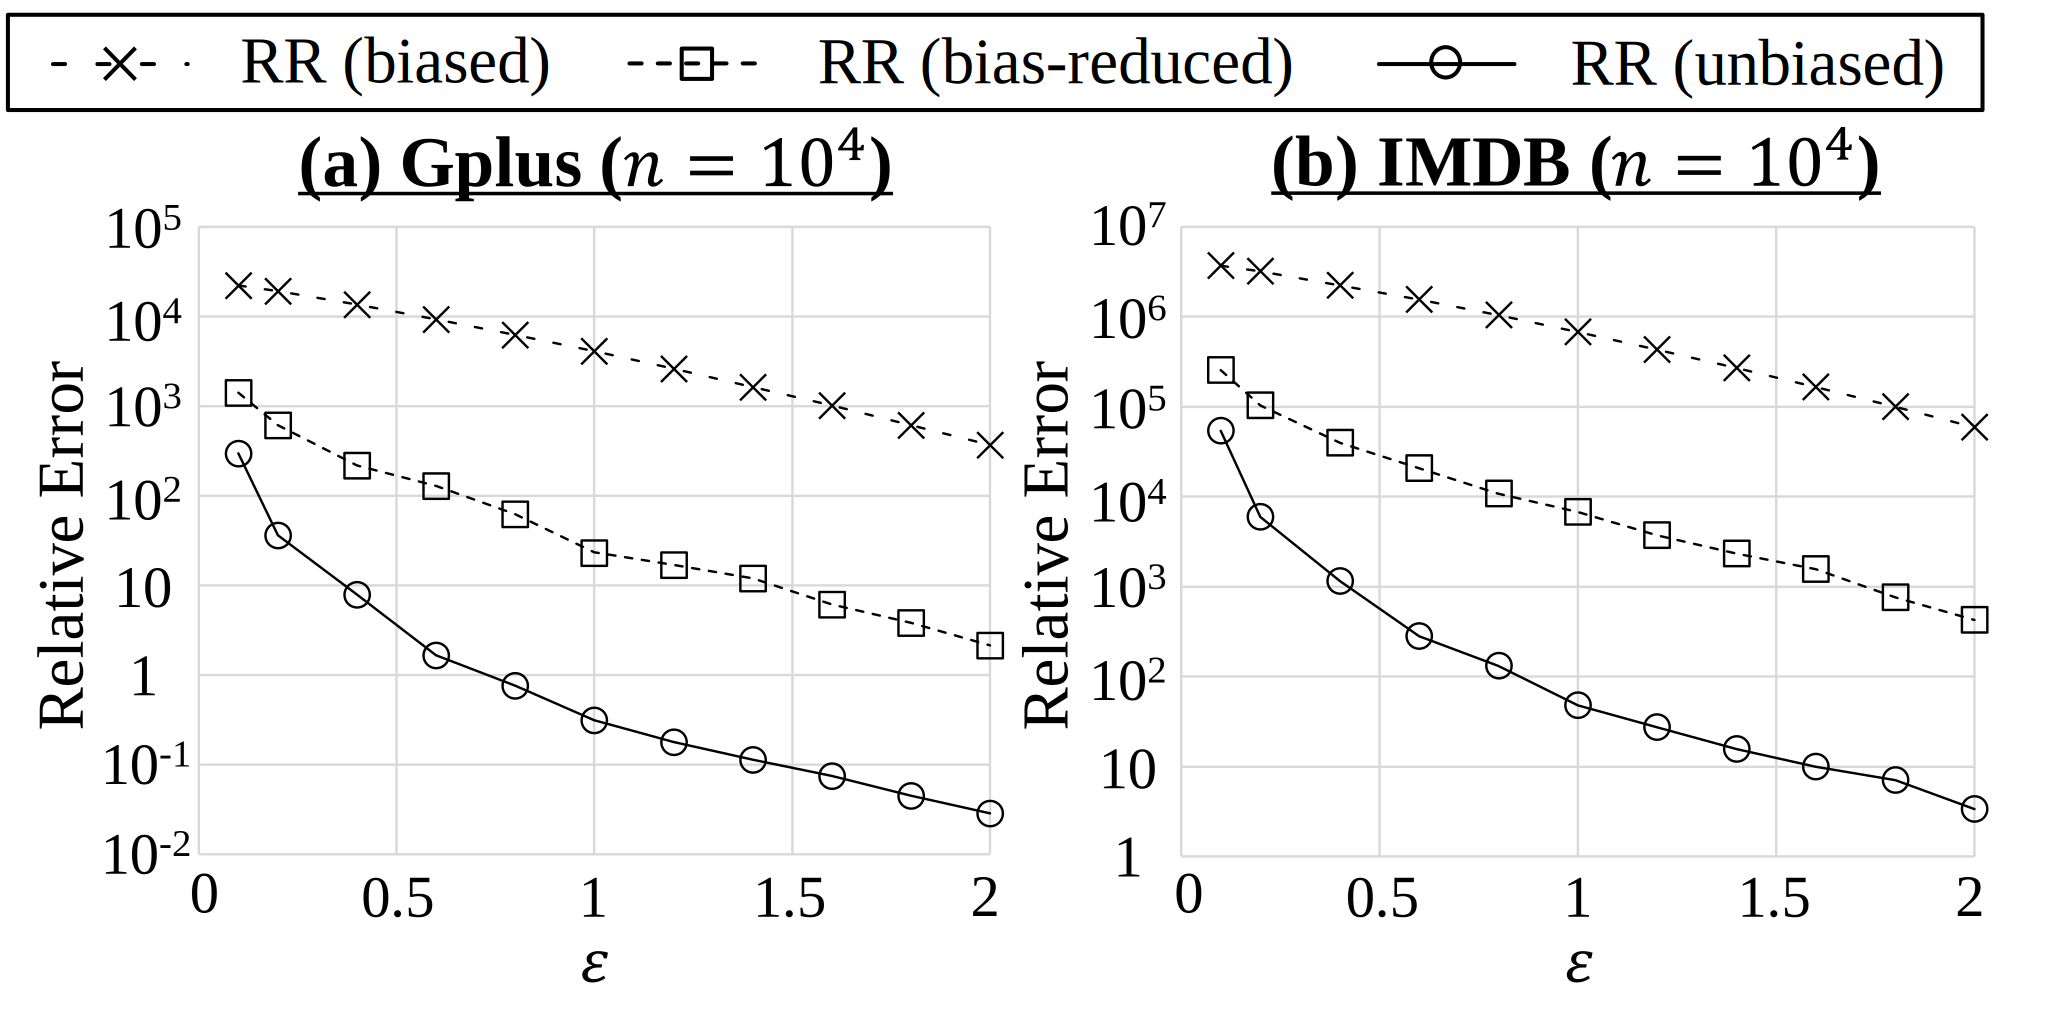
\includegraphics[width=0.99\linewidth]{fig/resB_one_round_small.pdf}
  
  \caption{Relative error of one-round algorithms for small datasets ($n=10000$).}
  \label{chap2-fig:resB_small}
\end{figure}

Figure~\ref{chap2-fig:resB_small} shows the results.
\textsf{RR (bias-reduced)} significantly outperforms \textsf{RR (biased)} and is significantly outperformed by \textsf{RR (unbiased)}.
We believe 
% that 
this is caused by the fact that \textsf{RR (bias-reduced)} introduces some approximation and does not calculate an unbiased estimate of $f_\triangle(G)$.

\smallskip
\noindent{\textbf{Large Datasets.}}~~Based on Figure~\ref{chap2-fig:resB_small}, we improve the time complexity of \textsf{RR (unbiased)} using the ARR and compare it with our two-rounds algorithms in large datasets.

Specifically, \textsf{RR (unbiased)} counts \textit{triangles}, \textit{$2$-edges} (three nodes with two edges), \textit{$1$-edges} (three nodes with one edge), and \textit{no-edges} (three nodes with no edges) in $G'$ obtained by Warner's RR.
Let $m_3, m_2, m_1, m_0 \in \nnints$ be the numbers of triangles, $2$-edges, $1$-edges, and no-edges, respectively, after applying Warner's RR.
\textsf{RR (unbiased)} calculates an unbiased estimate of $f_\triangle(G)$ from these four values.
Thus, we improve \textsf{RR (unbiased)} by using the ARR, which samples each edge with probability $p_2$ after Warner's RR, and then calculating unbiased estimates of $m_3$, $m_2$, $m_1$, and $m_0$.

Let $\hat{m}_3, \hat{m}_2, \hat{m}_1, \hat{m}_0 \in \reals$ be the unbiased estimates of $m_3$, $m_2$, $m_1$, and $m_0$, respectively. 
% after applying Warner's RR.
Let $m_3^*, m_2^*, m_1^*, m_0^* \in \nnints$ be the number of triangles, 2-edges, 1-edges, no-edges, respectively, after applying the ARR.
Since the ARR samples each edge with probability $p_2$, we obtain:
\begin{align*}
    m_3^* &= \textstyle{p_2^3 \hat{m}_3} \\
    m_2^* &= \textstyle{3p_2^2(1-p_2) \hat{m}_3 + p_2^2 \hat{m}_2} \\
    m_1^* &= \textstyle{3p_2(1-p_2)^2 \hat{m}_3 + 2p_2(1-p_2) \hat{m}_2 + p_2 \hat{m}_1.}
\end{align*}
By these equations,
% and $\hat{m}_3 + \hat{m}_2 + \hat{m}_1 + \hat{m}_0 = \frac{n(n-1)(n-2)}{6}$,
we obtain:
\begin{align}
    \hat{m}_3 &= \textstyle{\frac{m_3^*}{p_2^3}} \label{chap2-eq:hm_3} \\
    \hat{m}_2 &= \textstyle{\frac{m_2^*}{p_2^2} - 3(1-p_2)\hat{m}_3} \label{chap2-eq:hm_2} \\
    \hat{m}_1 &= \textstyle{\frac{m_1^*}{p_2} - 3(1-p_2)^2\hat{m}_3 - 2(1-p_2)\hat{m}_2} \label{chap2-eq:hm_1} \\
    \hat{m}_0 &= \textstyle{\frac{n(n-1)(n-2)}{6} - \hat{m}_3 - \hat{m}_2 - \hat{m}_1.} \label{chap2-eq:hm_0}
\end{align}
Therefore, after applying the ARR to the lower triangular part of $\bmA$, the server counts $m_3^*$, $m_2^*$, $m_1^*$, and $m_0^*$ in $G'$, and then calculates the unbiased estimates $\hat{m}_3$, $\hat{m}_2$, $\hat{m}_1$, and $\hat{m}_0$ by (\ref{chap2-eq:hm_3}), (\ref{chap2-eq:hm_2}), (\ref{chap2-eq:hm_1}), and (\ref{chap2-eq:hm_0}), respectively.
Finally, the server estimates $f_\triangle(G)$ from $\hat{m}_3$, $\hat{m}_2$, $\hat{m}_1$, and $\hat{m}_0$ in the same way as \textsf{RR (unbiased)}.
We denote this algorithm by \textsf{ARR (unbiased)}.
The time complexity of \textsf{ARR (unbiased)} is $O(\mu^3 n^3)$, where $\mu$ is the ARR parameter.

We compared \textsf{ARR (unbiased)} with our three algorithms with double clipping using \GPlus{} ($n=107614$) and \IMDB{} ($n=896308$).
For the sampling probability $p_2$, we set $p_2 = 10^{-3}$ or $10^{-6}$.
We averaged the relative error over $10$ runs.

\begin{figure}[t]
  \centering
  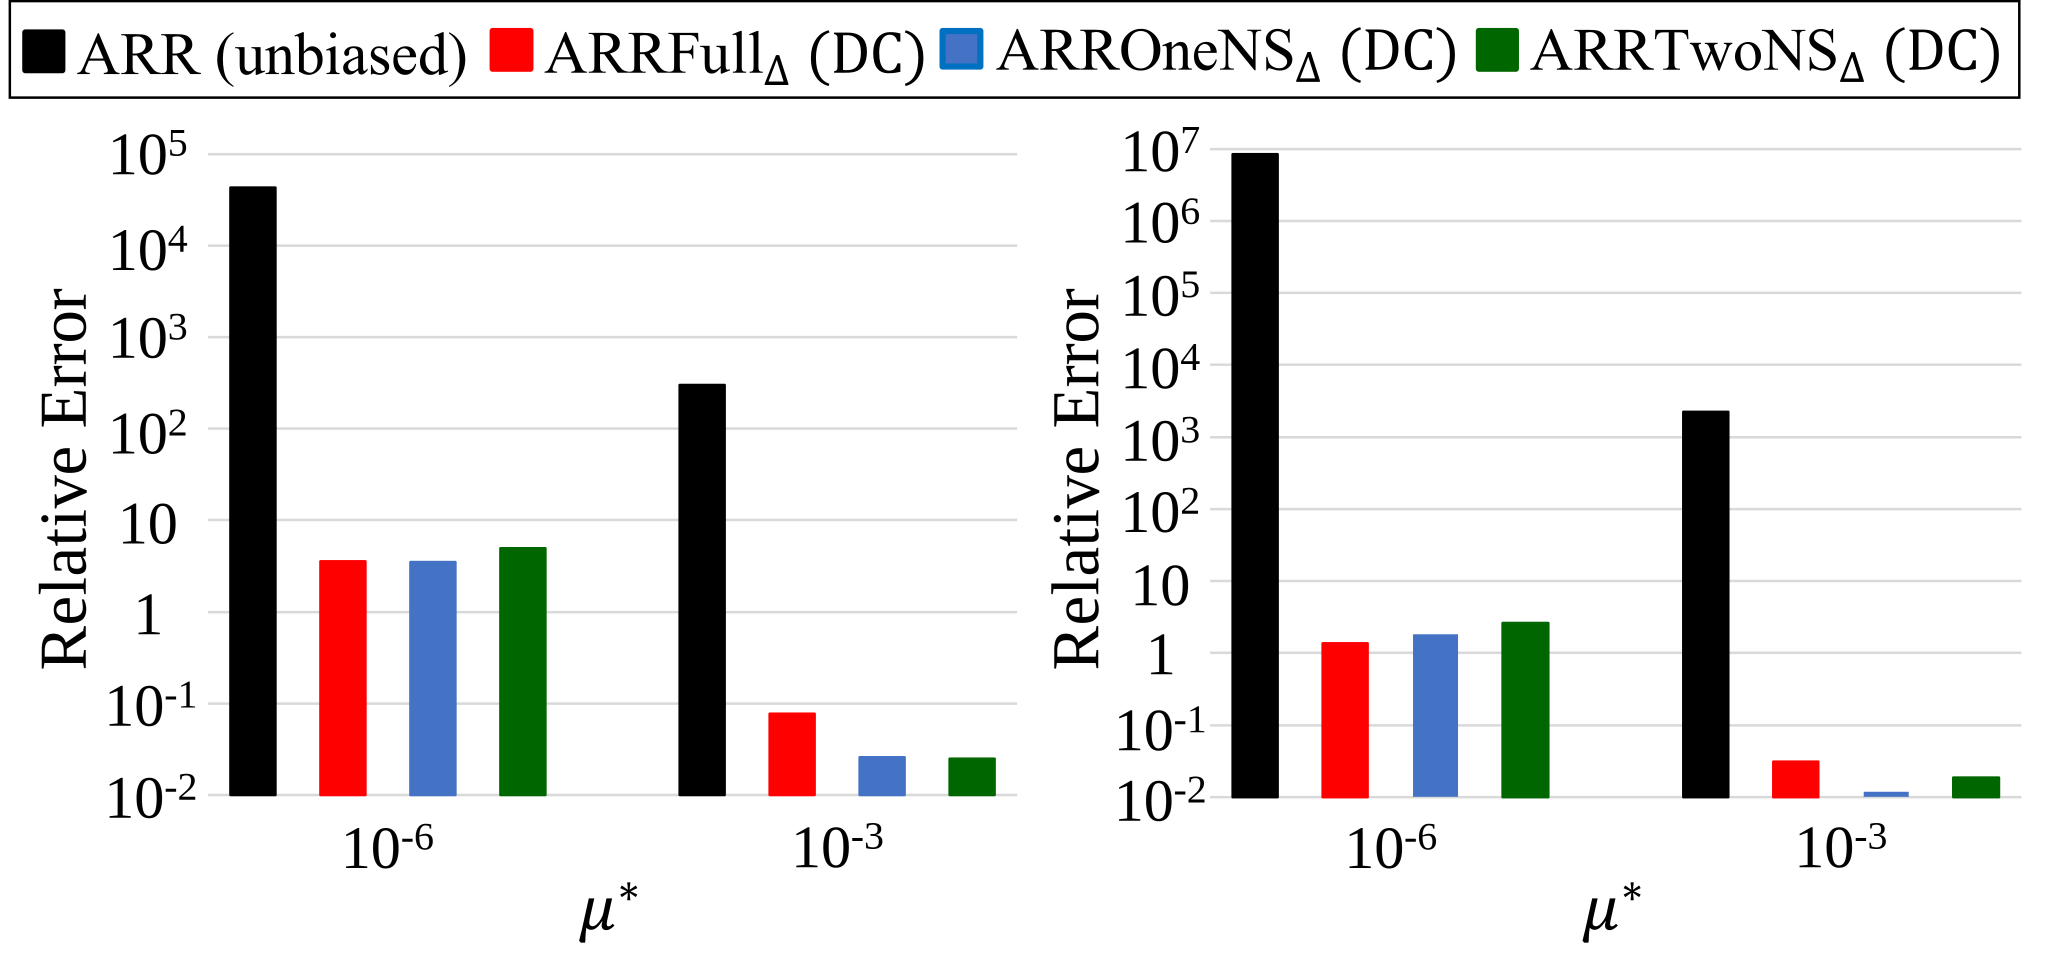
\includegraphics[width=0.99\linewidth]{fig/resB_one_round_large.pdf}
  
  \caption{Relative error of the one-round algorithm \textsf{ARR (unbiased)} and our three two-rounds algorithms with double clipping for large datasets ($n=107614$ in \GPlus{}, $n=896308$ in \IMDB{}).}
  \label{chap2-fig:resB_large}
\end{figure}

Figure~\ref{chap2-fig:resB_large} shows the results, where we set
% $\mu_F$ ($=\mu_o^2=\mu_T^3$)
$\mu^* = 10^{-6}$ or $10^{-3}$.
In \textsf{ARR (unbiased)}, we used $\mu^*$ as 
% a parameter $\mu$ of the ARR.
the ARR parameter $\mu$. 
Thus, we can see \textit{how much the relative error is reduced by introducing an additional round with \AlgOne{}}.
Figure~\ref{chap2-fig:resB_large} shows that the relative error of \textsf{ARR (unbiased)} is prohibitively large; i.e., relative error $\gg 1$.
% even when $\mu_F = 10^{-3}$.
This is because three edges are noisy in any noisy triangle. 
% and edge sampling is introduced to reduce the time complexity. 
% (recall that the one-round algorithms without sampling would require about $35$ years when $n=10^6$ \cite{Imola_USENIX21}).
% The relative error is extremely large when $\mu_F = 10^{-6}$ due to a very small sampling probability.
The relative error is significantly reduced by  introducing an additional round
% and counting noisy triangles in which only one edge is noisy.
% In contrast, our algorithms achieve much smaller estimation error
because only one edge is noisy in each noisy triangle at the second round.

In summary, one-round algorithms are far from acceptable in terms of the estimation error for large graphs, and two-round algorithms such as ours are necessary.

\section{Clustering Coefficient}
\label{chap2-sec:cluster}
% \smallskip
% \noindent{\textbf{Clustering Coefficient.}}~~We
Here we
% We have so far evaluated the estimation error of the triangle count.
% finally
% show that our algorithms are very useful for estimating the clustering coefficient.
evaluate the estimation error of the clustering coefficient using our algorithms.

% evaluated the estimation error of the clustering coefficient as follows.
We first estimated a triangle count by using our \AlgTwo{} with double clipping
($\epsilon_0 = \frac{\epsilon}{10}$ and
$\epsilon_1 = \epsilon_2 = \frac{9\epsilon}{20}$)
because it provides the best performance in Figures~\ref{chap2-fig:res2_w_Lap_abst}, \ref{chap2-fig:res2_w_Lap}, and \ref{chap2-fig:res3_n}.
Then we estimated a $2$-star count by
% a modified version of the algorithm in~\cite{Imola_USENIX21} using the adaptive edge clipping in Section~\ref{chap2-sec:double_clip}.
using the one-round $2$-star algorithm in~\cite{Imola_USENIX21} with the
% adaptive
edge clipping in Section~\ref{chap2-sec:double_clip}.

Specifically, we calculated a noisy degree $\td_i$ of each user $v_i$ 
% (possibly with edge clipping) 
by using the edge clipping with the privacy budget $\epsilon_0$.
Then we calculated the number $r_i \in \nnints$ of $2$-stars of which user $v_i$ is a center, and added $\Lap(\frac{\Delta}{\epsilon_1})$ to $r_i$, where $\Delta = \binom{\td_i}{2}$.
Let $\hr_i = r_i + \Lap(\frac{\Delta}{\epsilon_1})$ be the noisy $2$-star of $v_i$.
Finally, we calculated
% the sum of the noisy $2$-stars
the sum $\sum_{i=1}^n \hr_i$ as an estimate of the $2$-star count.
This $2$-star algorithm provides ($\epsilon_0 + \epsilon_1$)-edge privacy (see~\cite{Imola_USENIX21} for details).
For the privacy budgets $\epsilon_0$ and $\epsilon_1$, we set $\epsilon_0 = \frac{\epsilon}{10}$ and $\epsilon_1 = \frac{9\epsilon}{10}$.

Based on the triangle and $2$-star counts, we estimated the clustering coefficient as
$\frac{3 \times \hf_\triangle(G)}{\hf_{2\star}(G)}$,
% $3 \times \hf_\triangle(G) / \hf_{2\star}(G)$,
where $\hf_\triangle(G)$ (resp.~$\hf_{2\star}(G)$) is the estimate of the triangle (resp.~$2$-star) count.

\begin{figure}[t]
  \centering
  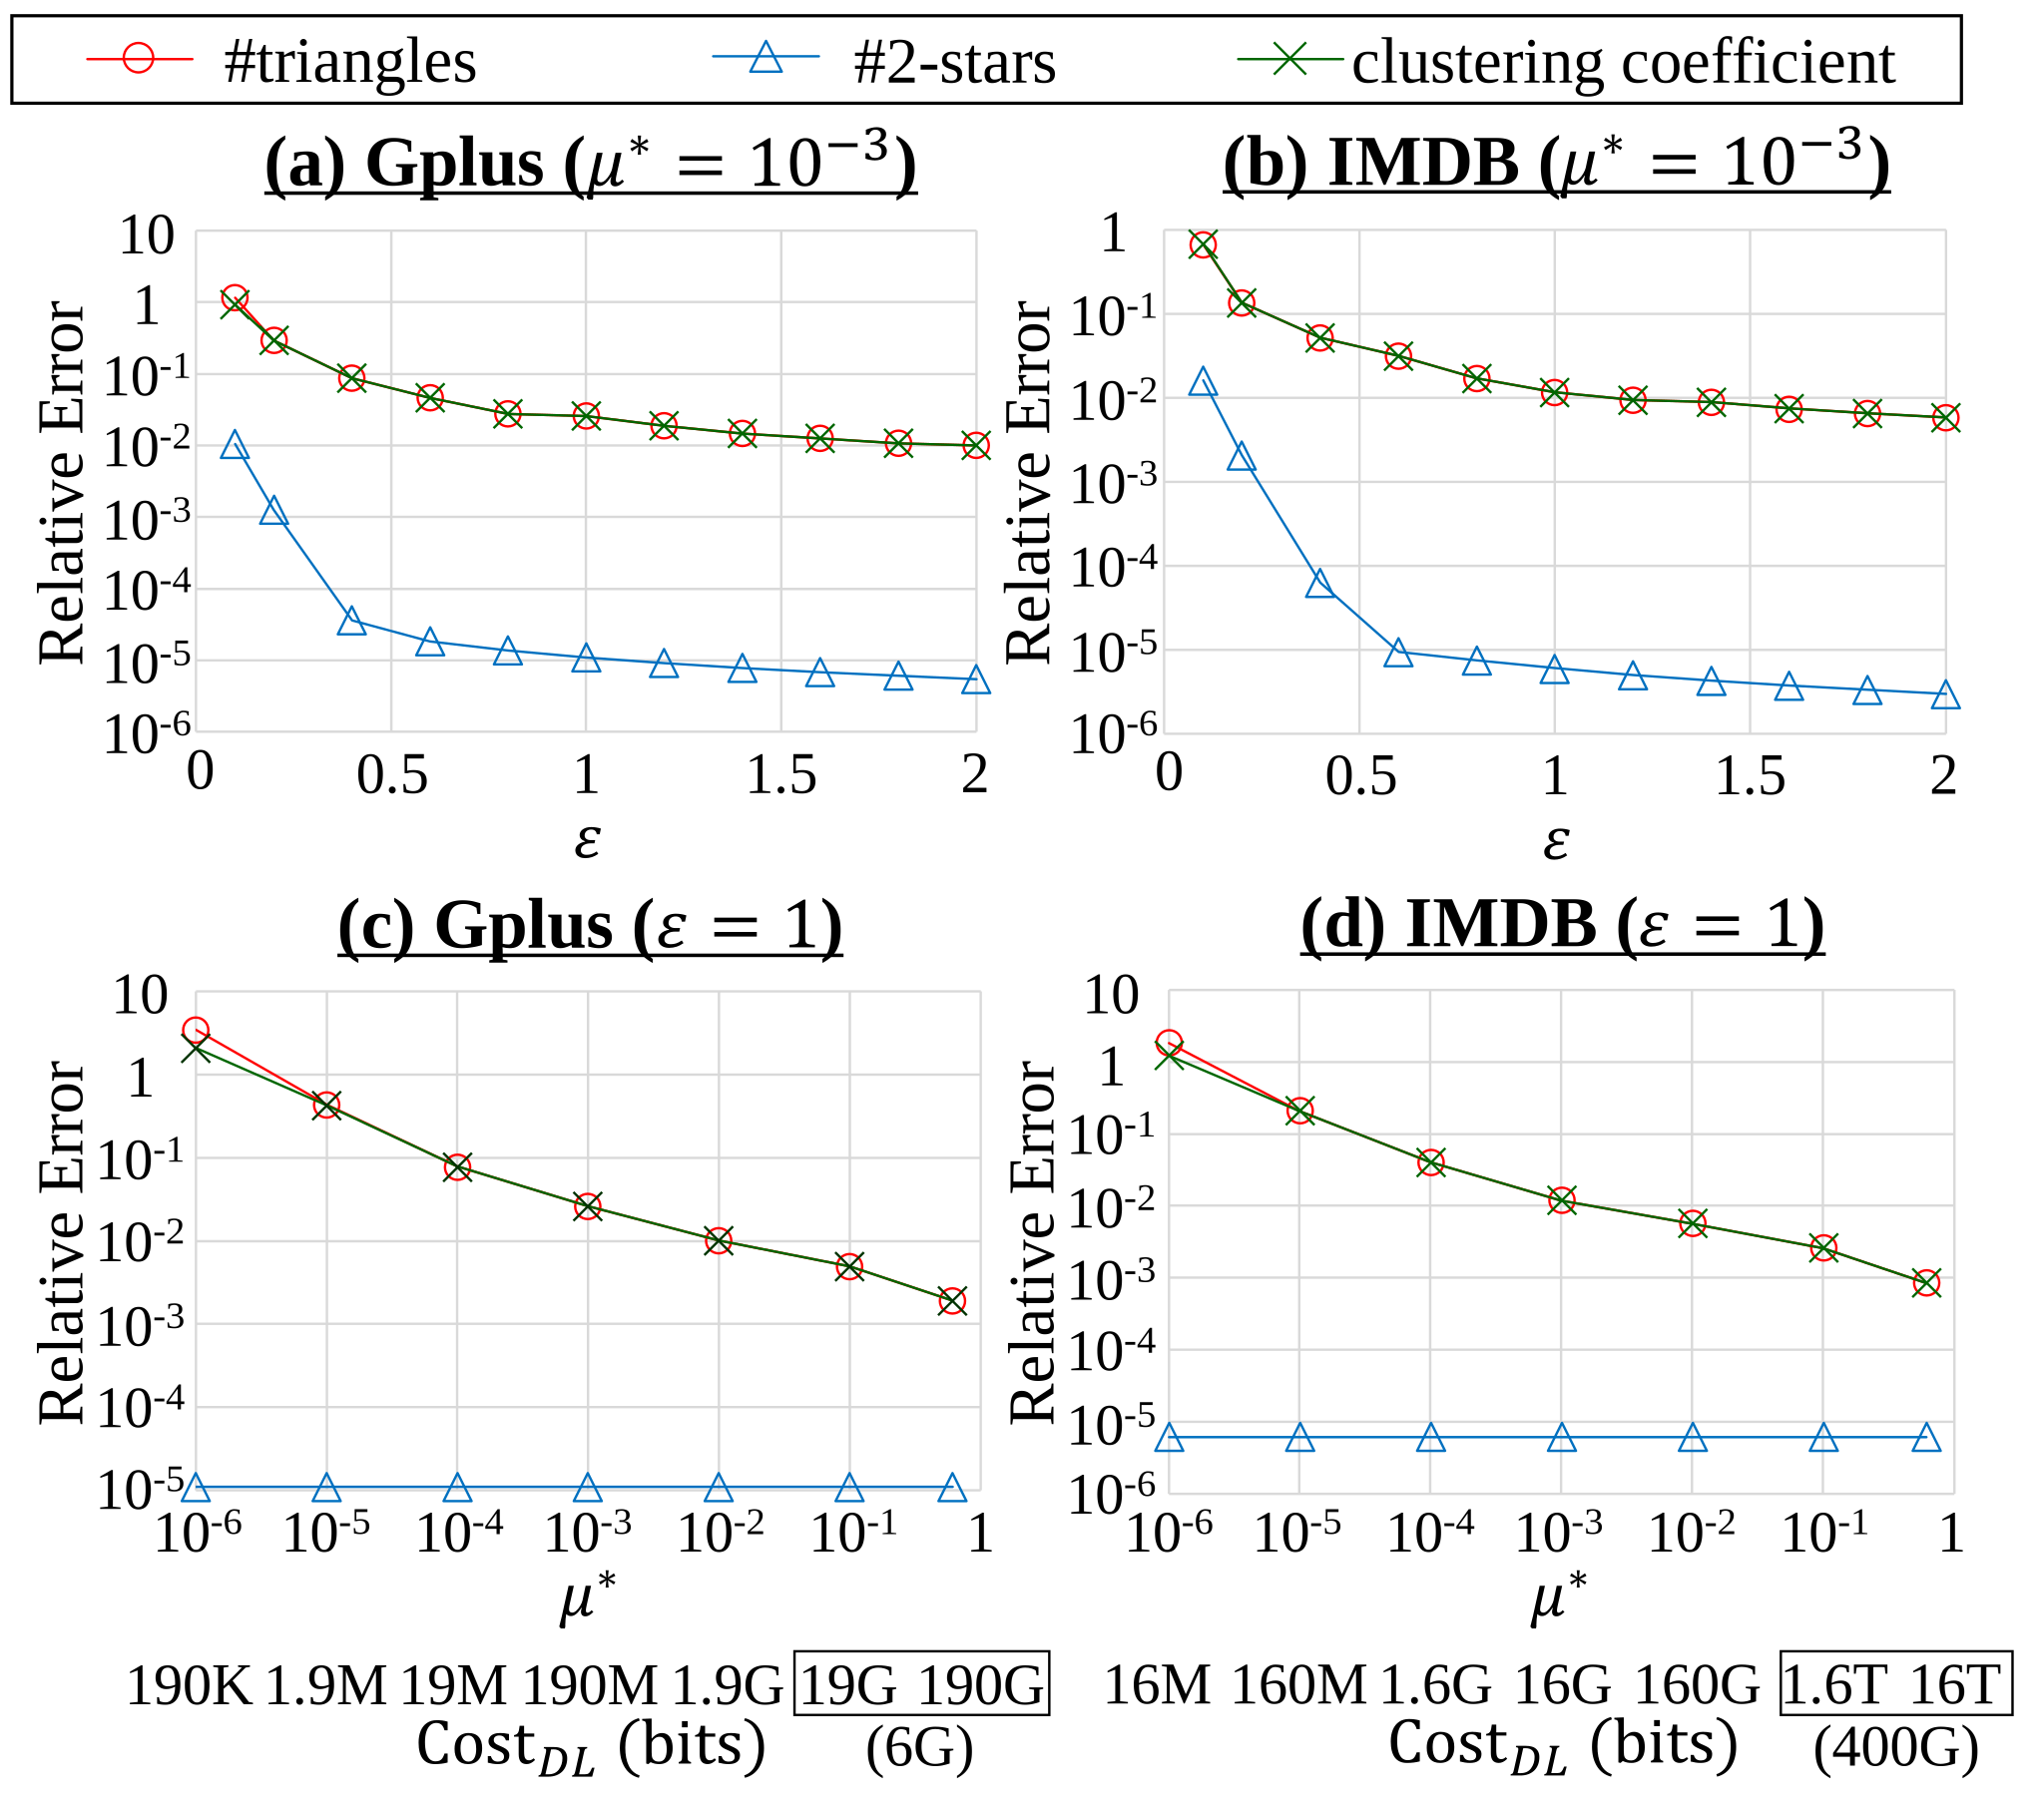
\includegraphics[width=0.99\linewidth]{fig/res5_cluster.pdf}
  
  \caption{Relative errors of \#triangles, \#$2$-stars, and the clustering coefficient in \AlgTwo{} with double clipping.
  $\CostDL$ is calculated by (\ref{chap2-eq:CostDL_F})
  (when $\mu^* \geq 0.1$,
  $\CostDL$ can be $6$ Gbits and $400$ Gbits in \GPlus{} and \IMDB{}, respectively).
  }
  \label{chap2-fig:res5_cluster}
\end{figure}

Figure~\ref{chap2-fig:res5_cluster} shows the relative errors of the triangle count, $2$-star count, and clustering coefficient.
Note that the relative error of the 2-star count is not changed by changing
% $\mu_F$ ($=\mu_O^2=\mu_T^3$)
$\mu^*$
because the 2-star algorithm does not use the ARR.
Figure~\ref{chap2-fig:res5_cluster} shows that the relative error of the $2$-star count is much smaller than that of the triangle count.
This is because each user can count her 2-stars locally (whereas she cannot count her triangles), as described in Section~\ref{chap2-sec:intro}.
Consequently, the relative error of the clustering coefficient is almost the same as that of the triangle count, as the denominator $\hf_{2\star}(G)$ in the clustering coefficient is very accurate.

Note that the clustering coefficient requires the privacy budgets for
calculating both $\hf_\triangle(G)$ and $\hf_{2\star}(G)$
% both the triangle count and $2$-star count
(in Figure~\ref{chap2-fig:res5_cluster}, $2\epsilon$ in total).
% $2\epsilon$ because it needs both the triangle count and $2$-star count.
However, we can accurately
% estimate the $2$-star count
calculate $\hf_{2\star}(G)$
with a very small privacy budget, as shown in Figure~\ref{chap2-fig:res5_cluster}.
Thus, we can accurately estimate the clustering coefficient with almost the same privacy budget as
the triangle count
% $\hf_\triangle(G)$
% by making the privacy budget for the $2$-star count small (e.g., $\epsilon=0.1$ or $0.2$).
by assigning a very small privacy budget (e.g., $\epsilon=0.1$ or $0.2$) for
% the $2$-star count.
$\hf_{2\star}(G)$.

In summary, we can accurately estimate the clustering coefficient as well as the triangle count under edge LDP by using our \AlgTwo{} with double clipping.

\arxiv{
\section{Experiments Using the Barab\'{a}si-Albert Graph Datasets}
\label{chap2-sec:BAmodel}
In Section~\ref{chap2-sec:experiments}, we evaluated our algorithms using two real datasets.
Below we also evaluate our algorithms using a synthetic graph based on the BA (Barab\'{a}si-Albert) graph model~\cite{NetworkScience}, which has a power-law degree distribution.

In the BA graph model, a graph of $n$ nodes is generated by attaching new nodes one by one.
% Each node has $m \in \nnints$ edges, 
Each new node is connected to $m \in \nnints$ existing nodes, 
and each edge is connected to an existing node with probability proportional to its degree.
We used NetworkX \cite{Hagberg_SciPy08}, a Python package for complex networks, to generate synthetic graphs based on the BA graph model.

We generated a graph $G=(V,E)$ with the same number of nodes as
% the Google+ dataset~\cite{McAuley_NIPS12} (\GPlus{});
\GPlus{}; i.e., $n=107614$ nodes.
% and $m=$
For the number $m$ of edges per node, we set $m=50$, $114$, or $500$.
% Note that the BA graph with $m=114$ has almost the average degree as \GPlus{}.
% When $m=114$, most nodes have the degree of $114$, which is the average degree in \GPlus{}. 
% Thus, we can see the difference between them.
Using these graphs, we evaluated our three algorithms with double clipping.
We set parameters in the same as Section~\ref{chap2-sec:experiments}; i.e.,
$\alpha = 150$, $\beta = 10^{-6}$, $\epsilon_0 = \frac{\epsilon}{10}$, and $\epsilon_1 = \epsilon_2 = \frac{9\epsilon}{20}$.
% We ran each algorithm $10$ times, and averaged the relative error over the $10$ cases.
For each algorithm, we averaged the relative error over $10$ runs.

% \begin{figure}[t]
%   \centering
%   
\includegraphics[width=0.95\linewidth]{fig/subgraphs.pdf}
%   
%   \caption{Subgraphs used in our theoretical analysis.}
%   \label{chap2-fig:subgraphs}
% \end{figure}

Figure~\ref{chap2-fig:resA_BAGraph} shows the results, where $\epsilon=1$ and
% $\mu_F$ ($= \mu_O^2 = \mu_T^3$)
$\mu^* = 10^{-3}$.
We observe that \AlgTwo{} significantly outperforms \AlgOne{} and \AlgThree{} when $m=500$, and that \AlgTwo{} performs almost the same as \AlgOne{} when $m=50$ or $114$.

To examine the reason for this, we also decomposed the estimation error into two components (the first error by empirical estimation and the second error by the Laplacian noise) in the same way as Figure~\ref{chap2-fig:res3_emp_Lap}.
Figure~\ref{chap2-fig:resA_BAGraph_emp_Lap} shows the results.
% In addition, we calculated the number $C_4$ of $4$-cycles in the BA graph.
We also show in Table~\ref{chap2-tab:resA_4cycles} the number $C_4$ of $4$-cycles in each BA graph ($m=50$, $114$, or $500$) and \GPlus{}.

From Figure~\ref{chap2-fig:resA_BAGraph_emp_Lap} and Table~\ref{chap2-tab:resA_4cycles}, we can explain Figure~\ref{chap2-fig:resA_BAGraph} as follows.
The BA graphs with $m=50$ and $114$ have a much smaller number $C_4$ of $4$-cycles than \GPlus{}, as shown in Table~\ref{chap2-tab:resA_4cycles}.
Consequently,
% the error caused by
the Laplacian noise is relatively large and dominant for these two graphs, as shown in Figure~\ref{chap2-fig:resA_BAGraph_emp_Lap}.
In particular,
% the relative error of
the Laplacian noise is the largest in \AlgThree{} because it cannot effectively reduce the global sensitivity by double clipping, as explained in Section~\ref{chap2-sec:double_clip}.
In contrast, the BA graph with $m=500$ has a larger number $C_4$ of $4$-cycles than \GPlus{}, and therefore the Laplacian noise is not dominant (except for \AlgThree{}).
This explains the results in Figure~\ref{chap2-fig:resA_BAGraph}.

These results
% , along with Section~\ref{chap2-sec:experiments},
% Our experimental results in Appendix~\ref{chap2-sec:BAmodel} and Section~\ref{chap2-sec:experiments},
show that \AlgTwo{} outperforms \AlgOne{} especially when the number $C_4$ of $4$-cycles is large.
As we have shown in Section~\ref{chap2-sec:experiments} and Appendix~\ref{chap2-sec:BAmodel}, $C_4$ is large in a large graph (e.g., $n \approx 10^6$) or dense graph (e.g., \GPlus{}, BA graph with $m=500$).

\begin{figure}[t]
  \centering
  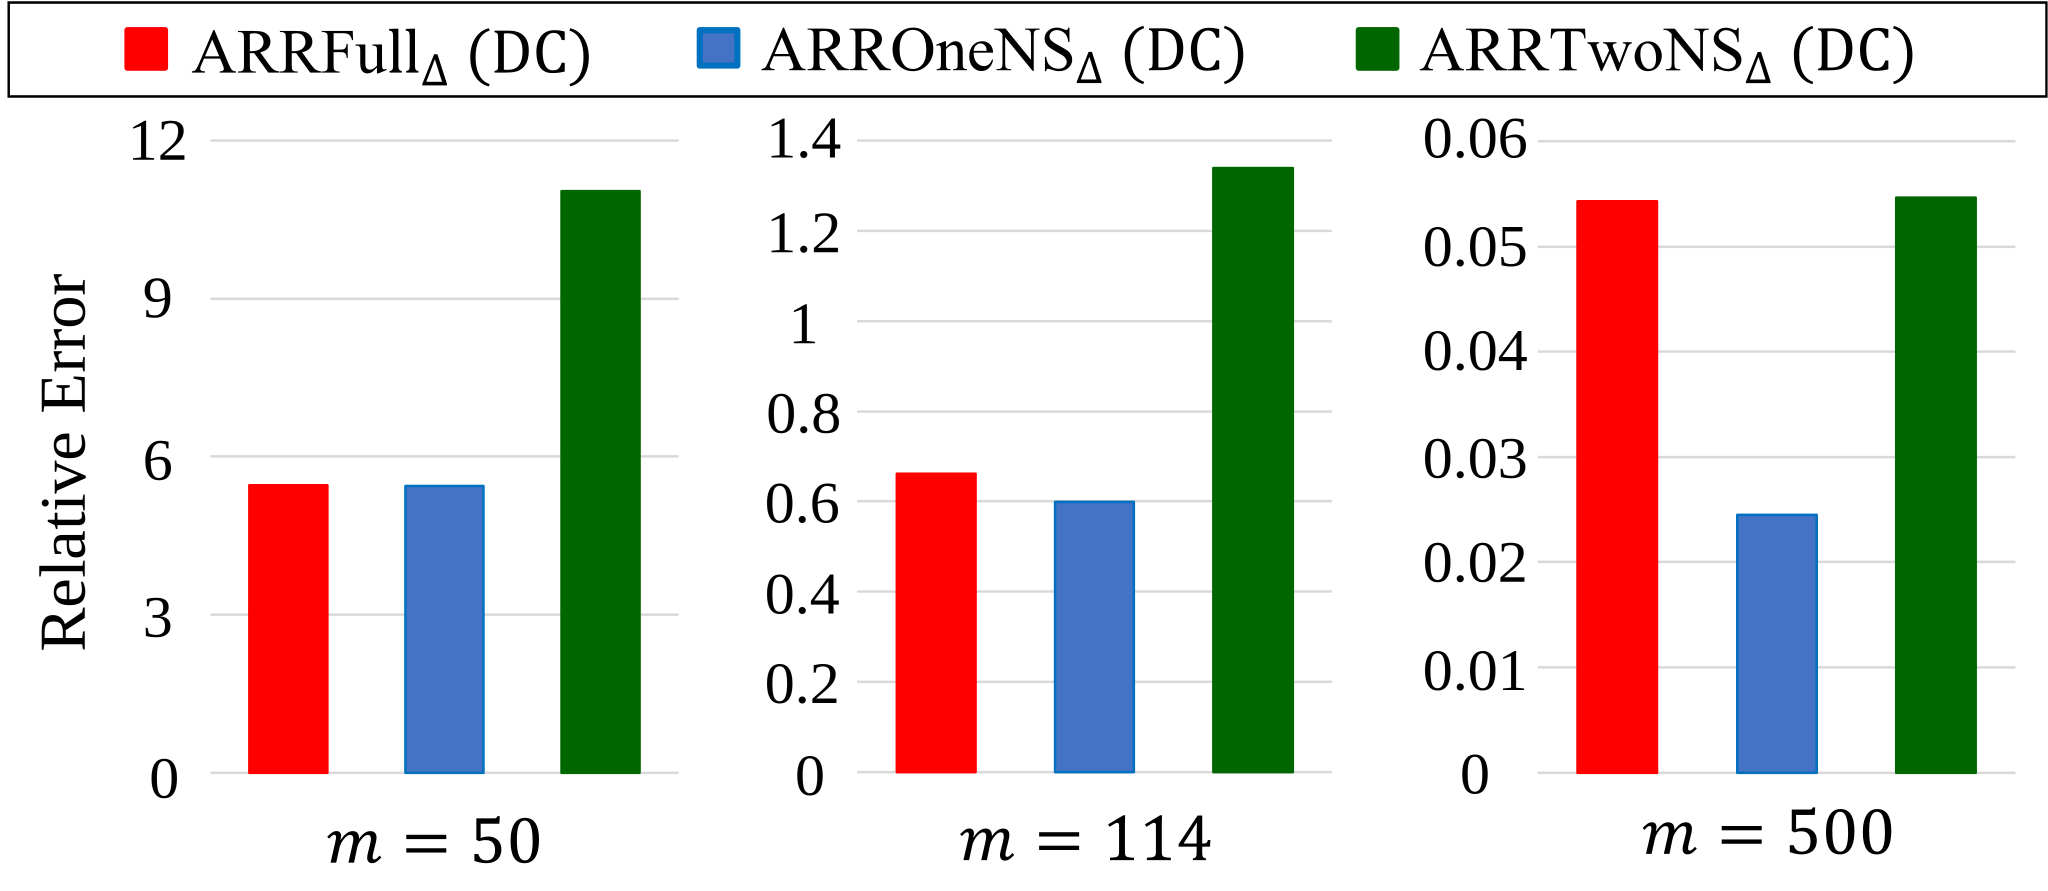
\includegraphics[width=0.99\linewidth]{fig/resA_BAGraph.pdf}
  
  \caption{Relative error of our three algorithms with double clipping in the BA graphs ($n=107614$, $\epsilon=1$, $\mu^* = 10^{-3}$).}
  \label{chap2-fig:resA_BAGraph}
% \end{figure}
\vspace{5mm}
% \begin{figure}[t]
  \centering
  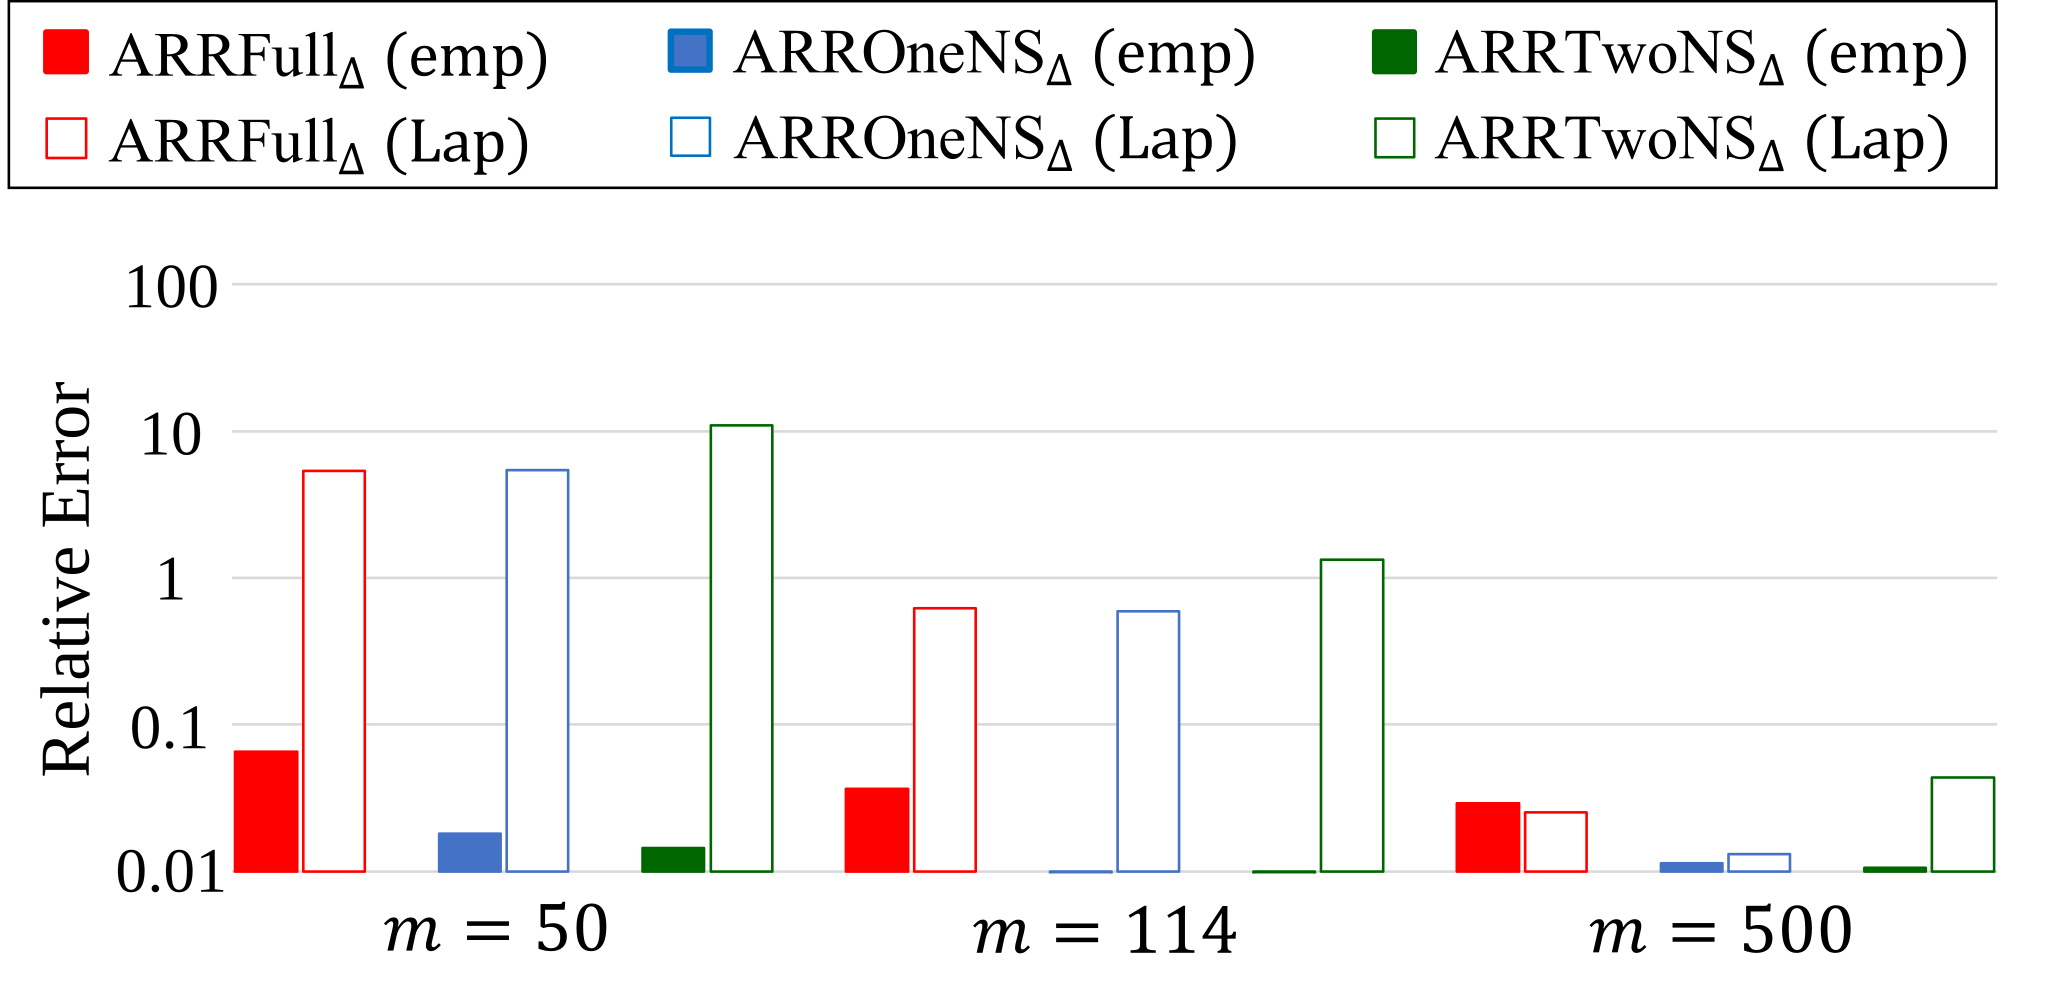
\includegraphics[width=0.95\linewidth]{fig/resA_BAGraph_emp_Lap.pdf}
  
  \caption{Relative error of empirical estimation and the Laplacian noise in our three algorithms with double clipping in the BA graphs ($n=107614$, $\epsilon=1$, $\mu^* = 10^{-3}$).}
  \label{chap2-fig:resA_BAGraph_emp_Lap}
\end{figure}

\section{Edge Clipping and Noisy Triangle Clipping}
\label{chap2-sec:EC_DC}
% \smallskip
% \noindent{\textbf{Edge Clipping and Noisy Triangle Clipping.}}~~
In Section~\ref{chap2-sec:experiments}, we showed that our double clipping significantly reduces the estimation error.
To investigate the effect of
% adaptive
edge clipping and noisy triangle clipping independently, we also performed the following ablation study.

We evaluated our three algorithms with only
% adaptive
edge clipping; i.e., each user calculates a noisy degree $\td_i$ (possibly with edge clipping) and then adds $\Lap(\frac{\td_i}{\epsilon_2}$) to her noisy triangle count.
Then we compared them with our algorithms with double clipping and without clipping.

\begin{table}[t]
\caption{\#$4$-cycles $C_4$ in each graph dataset.}
\centering
\hbox to\hsize{\hfil
\begin{tabular}{l|l|l|l|l}
\hline
		&	$m=50$   &  $m=114$   &  $m=500$   &  \GPlus{}\\
\hline
$C_4$   &   $8.8 \times 10^8$ &  $1.7 \times 10^{10}$ &   $3.1 \times 10^{12}$ &   $2.8 \times 10^{12}$\\
\hline
\end{tabular}
\hfil}
\label{chap2-tab:resA_4cycles}
\end{table}

\begin{figure}[t]
  \centering
  \includegraphics[width=0.99\linewidth]{fig/res2_w_Lap_EC.pdf}
  
  \caption{Relative error of our three algorithms without clipping (``$d_{max}$''), with only edge clipping (``EC''), and double clipping (``DC'') when $\epsilon=1$ and $\mu^* = 10^{-6}$ or $10^{-3}$ ($n=107614$ in \GPlus{}, $n=896308$ in \IMDB{}).}
  \label{chap2-fig:res2_w_Lap_EC}
\end{figure}

Figure~\ref{chap2-fig:res2_w_Lap_EC} shows the results, where $\epsilon=1$, $\mu^* = 10^{-6}$ or $10^{-3}$, and ``EC'' represents our algorithms with only
% adaptive
edge clipping.
We observe that ``EC''
% (only edge clipping)
outperforms ``$d_{max}$'' (w/o clipping) and is outperformed by ``DC'' (double clipping).
The difference between ``EC'' and ``DC'' is significant especially when $\mu^* = 10^{-6}$ (``DC'' is smaller than $\frac{1}{100}$ of ``EC'').
This is because our noisy triangle clipping reduces the global sensitivity by using a small value of
$\mu^*$. 
% $\mu_F$ ($=\mu_O^2 = \mu_T^3$).
From Figure~\ref{chap2-fig:res2_w_Lap_EC}, we conclude that each component (i.e.,
% adaptive
edge clipping, noisy triangle clipping) is essential in our double clipping.

\section{Proof of Proposition~\ref{chap2-prop:seq_comp_edge_LDP}}
\label{chap2-sec:proof_seq_comp_edge_LDP}
Let $\calR_i(\bma_i) = (\calR_i^1(\bma_i), \calR_i^2(M_i)(\bma_i))$ be the
randomizer used by user $v_i$ in the composition. To establish that
$\calR_i(\bma_i)$ satisfies $\epsilon$-edge LDP for every $v_i \in V$, we will
prove that~\eqref{chap2-eq:edge_LDP} holds for $\calR_i(\bma_i)$. To do this, first write
\begin{align*}
  &\;\Pr[(\calR_i^1(\bma_i), \calR_i^2(M_i)(\bma_i)) = (r_i^1, r_i^2)] = \\
  &\qquad\Pr[\calR_i^1(\bma_i) = r_i^1]\Pr[\calR_i^2(M_i)(\bma_i) = r_i^2 | \calR_i^1(\bma_i) = r_i^1] \\
  &\qquad\Pr[\calR_i^1(\bma_i) = r_i^1]\Pr[\calR_i^2(M_i)(\bma_i) = r_i^2 | M_i = \lambda_i(r_i^1)],
\end{align*}
where the last equality follows because $M_i = \lambda_i(\calR_i^1(\bma_i))$ for a post-processing algorithm $\lambda_i$.
Notice that the same equalities are true when we replace $\bma_i$ with $\bma_i'$.
Because $\calR_i^1$ and $\calR_i^2(M_i)$ (for any $M_i$) satisfy $\epsilon_1, \epsilon_2$-edge LDP, respectively,
we have
\begin{align*}
  &\;\Pr[\calR_i^1(\bma_i) = r_i^1]\Pr[\calR_i^2(M_i)(\bma_i) = r_i^2 | M_i = \lambda_i(r_i^1)] \\
  &\qquad\leq e^{\epsilon_1}\Pr[\calR_i^1(\bma_i') = r_i^1]e^{\epsilon_2}\Pr[\calR_i^2(\bma_i') = r_i^2 | M_i = \lambda_i(r_i^1)] \\
  &\qquad= e^{\epsilon_1 + \epsilon_2} \Pr[(\calR_i^1(\bma_i'), \calR_i^2(M_i)(\bma_i')) = (r_i^1, r_i^2)].
\end{align*}
This establishes the result. \qed

\section{Proof of Statements in Section~\ref{chap2-sec:algorithms}}
\label{chap2-sec:proof_algorithms}
\subsection{Proof of Theorem~\ref{chap2-thm:privacy_algorithms}}
Let $\bma_i, \bma'_i \in \{0,1\}^n$ be two neighbor lists that differ in one bit.
Let $t'_i$, $s'_i$, and $w'_i$ be respectively the values of $t_i$ (line 11 of Algorithm~\ref{chap2-alg:unify}), $s_i$ (line 12), and $w_i$ (line 13) when the neighbor list of user $v_i$ is $\bma'_i$.
Let $\Delta w_i = |w'_i - w_i|$.
Then we have $t'_i - t_i \in [0,d_{max}]$ and $s'_i - s_i \in [0,d_{max}]$, and therefore $\Delta w_i = |(t'_i - t_i) - \mu^* \rho(s'_i - s_i)| \leq d_{max}$.

Since we add
$\Lap\left(\frac{d_{max}}{\epsilon_2}\right)$
to $w_i$, the second round provides $\epsilon_2$-edge LDP.
The first round uses $ARR_{\epsilon_1,\mu}$ and provides $\epsilon_1$-edge LDP.
Thus, by sequential composition (Proposition~\ref{chap2-prop:seq_comp_edge_LDP}),
Algorithm~\ref{chap2-alg:unify} provides ($\epsilon_1+\epsilon_2$)-edge LDP in total.
It also provides ($\epsilon_1+\epsilon_2$)-relationship DP because it uses only the lower-triangular part of $\bmA$ (Proposition~\ref{chap2-prop:edge_LDP_entire_edge_LDP}).
% \ji{We should formally state the lower-triangular relationship DP result somewhere, I think maybe add it to proposition 1.}
\qed

\subsection{Proof of Theorem~\ref{chap2-thm:l2loss_algorithms}}
\label{chap2-sub:prrof_l2loss_algorithms}
% \paragraph{Unbiased Estimators}
% \smallskip
\noindent{\textbf{Unbiased Estimators.}}~~First, we will show that $\hf_\triangle(G)$ satisfies
$\E[\hf_\triangle(G)] = f_\triangle(G)$ for all $G \in \calG$, in \AlgOne{}, \AlgTwo{}, \AlgThree{}.
Regardless of algorithm, we have
\begin{align}
  &\;\E[\hf_\triangle(G)] \nonumber \\
  &= \frac{1}{\mu^*(1-\rho)}\sum_{i=1}^n \E[w_i] \nonumber \\
  &= \frac{1}{\mu^*(1-\rho)}\sum_{i=1}^n \E[t_i - \mu^* \rho s_i] \nonumber \\
  &= \frac{1}{\mu^*(1-\rho)}\sum_{i=1}^n \sum_{\substack{1 \leq j < k < i \leq n \\ a_{i,j} = a_{i,k} = 1}} \E[\textbf{1}_{(v_j, v_k) \in M_i} - \mu^* \rho],
  \label{chap2-eq:unbias_1}
\end{align}
where $\rho = e^{-\epsilon_1}$, and the quantites $\mu^*, t_i, s_i$ are defined in
Algorithm~\ref{chap2-alg:unify}. Given that $a_{i,j} = a_{i,k} = 1$, we have that
$\Pr[(v_i, v_j) \in E'] = \Pr[(v_i, v_k) \in E'] = \mu$ by definition of ARR.
Furthermore,
% $\Pr[(v_i, v_k) \in E'] = \mu$ if $a_{i,k} = 1$, and $\Pr[(v_i, v_k) \in E'] = \mu\rho$ otherwise.
$\Pr[(v_j, v_k) \in E'] = \mu$ if $a_{j,k} = 1$, and $\Pr[(v_j, v_k) \in E'] = \mu\rho$ otherwise.
Examining~\eqref{chap2-eq:M_i_I},~\eqref{chap2-eq:M_i_II}, and~\eqref{chap2-eq:M_i_III}, we have
\[
  \Pr[(v_j, v_k) \in M_i] =
  \begin{cases}
    \mu^* & a_{j,k} = 1 \\
    \mu^*\rho & a_{j,k} = 0
  \end{cases}
\]
for all the three algorithms (note that $\mu^* = \mu$, $\mu^2$, and $\mu^3$ in \AlgOne{}, \AlgTwo{}, \AlgThree{}, respectively).
Thus, $\E[\textbf{1}_{(v_j, v_k) \in M_i}] = \mu^* (\rho + (1-\rho) a_{j,k})$
($= \mu^*$ if $a_{i,j}=1$ and $\mu^* \rho$ if $a_{i,j}=0$).
Plugging into~\eqref{chap2-eq:unbias_1}, we have
\begin{align*}
  &\;\E[\hf_\triangle(G)] \\
  &=
  \frac{1}{\mu^*(1-\rho)}\sum_{i=1}^n \sum_{\substack{1 \leq j < k < i \leq n \\ a_{i,j} = a_{i,k} =
  1}} \mu^*(\rho + (1-\rho)a_{j,k}) - \mu^* \rho \\
  &= \frac{1}{\mu^*(1-\rho)}\sum_{i=1}^n \sum_{\substack{1 \leq j < k < i \leq n \\ a_{i,j} = a_{i,k} =
  1}} \mu^*(1-\rho)a_{j,k} \\
  &= \sum_{i=1}^n \sum_{\substack{1 \leq j < k < i \leq n \\ a_{i,j} = a_{i,k} =
  1}} a_{j,k} \\
  &= f_\triangle(G).
\end{align*} 
Thus, $\hf_\triangle(G)$ is unbiased. \qed

% \paragraph{$l_2^2$-Loss of Estimators}
\smallskip
\noindent{\textbf{$l_2$ Loss of Estimators.}}~~Using bias-variance decomposition, we have
for any graph $G$,
\begin{align*}
  l_2^2(f_\triangle(G), \hf_\triangle(G)) &= \E[(\hf_\triangle(G) - f_\triangle(G))^2] \\
  &= \E[(f_\triangle(G) - \E[\hf_\triangle(G)])^2] + \V[\hf_\triangle(G)] \\
  &= \V[\hf_\triangle(G)],
\end{align*}
where the last step follows because $\hf$ is unbiased.
Since $\hf_\triangle(G) = \frac{1}{\mu^*(1-\rho)} \sum_{i=1}^n \hw_i$, we have
% Substituting for $\hf_\triangle(G)$, we see
\begin{align}
  &\;\V[\hf_\triangle(G)] \nonumber \\
  &= \frac{1}{(\mu^*)^2(1-\rho)^2}\V\left[\sum_{i=1}^n \hw_i\right] \nonumber \\
  &= \frac{1}{(\mu^*)^2(1-\rho)^2}\V\left[\sum_{i=1}^n w_i + \Lap\left(\frac{d_{max}}{\epsilon_2} \right)\right] \nonumber \\
  &= \frac{1}{(\mu^*)^2(1-\rho)^2}\left(\V\left[\sum_{i=1}^n w_i\right] +
  n\V\left[\Lap\left(\frac{d_{max}}{\epsilon_2}\right)\right]\right) \nonumber \\
  &= \frac{1}{(\mu^*)^2(1-\rho)^2}\left(\V\left[\sum_{i=1}^n w_i\right] +
  2n\frac{d_{max}^2}{\epsilon_2^2}\right), \label{chap2-eq:inter_var}
\end{align}
where the
% third
fourth
line follows from independence of the added of Laplace noise.
Now, we will prove bounds on $\V[\sum_{i=1}^nw_i]$ for \AlgOne{}, \AlgTwo{}, and
\AlgThree{}. In the following, we let $S_k(G)$ be the number of $k$-stars in
$G$ and $C_4(G)$ be the number of $4$-cycles in $G$
% , and $P_3(G)$ be the number of
% $3$-paths in $G$.

% \paragraph{Bounding the Variance in \AlgOne{}}
\smallskip
\noindent{\textbf{Bounding the Variance in \AlgOne{}.}}~~In \AlgOne{}, $M_i$ is defined by \eqref{chap2-eq:M_i_I}. Thus we have
% we have $M_i = E'$, so we can write
\begin{align*}
  \sum_{i=1}^n w_i &= \sum_{i=1}^n \sum_{\substack{1 \leq j < k < i \leq n \\ a_{i,j} = 1, a_{i,k} = 1}} \textbf{1}_{(v_j, v_k) \in M_i} \\
  &= \sum_{1 \leq j < k \leq n} \sum_{k < i \leq n} a_{i,j} a_{i,k} \textbf{1}_{(v_j, v_k) \in E'} \\
  &= \sum_{1 \leq j < k \leq n} \textbf{1}_{(v_j, v_k) \in E'}\sum_{k < i \leq n} a_{i,j} a_{i,k}
\end{align*}
For $j < k$, we introduce the constant $c_{jk} = \sum_{k < i \leq n} a_{i,j} a_{i,k}$. Notice that
for any choice of $j$ and $k$, $\textbf{1}_{(v_j, v_k) \in E'}$ for $1 \leq j \leq k$ are mutually independent,
because all edges in $E'$ are mutually independent. Furthermore, the indicator
$\textbf{1}_{(v_j, v_k) \in E'}$ is a Bernoulli random variable with parameter
either $\mu$ or $\mu\rho$, and in either case, $\V[\textbf{1}_{(v_j, v_k) \in
E'}] \leq \mu$. We have
\begin{align*}
  \V\left[\sum_{i=1}^n w_i\right]
  &= \V\left[\sum_{1 \leq j < k \leq n} \textbf{1}_{(v_j, v_k) \in E'}c_{jk}\right] \\
  &= \sum_{1 \leq j < k \leq n} \V[\textbf{1}_{(v_j, v_k) \in E'}c_{jk}] \\
  &= \sum_{1 \leq j < k \leq n} \mu c_{jk}^2.
\end{align*}
By Lemma~\ref{chap2-lem:c_ij_4cycle_2star} (which is shown at the end of Appendix~\ref{chap2-sub:prrof_l2loss_algorithms}), we have $\sum_{1 \leq j < k \leq n} c_{jk}^2 \leq 2 C_4(G) + S_2(G)$.
Plugging into~\eqref{chap2-eq:inter_var} (and substituting $\mu^* = \mu$), we obtain
\begin{align*}
  \V[\hf_\triangle(G)]
  &= \frac{1}{(1-\rho)^2}\left(\frac{1}{\mu}(2C_4(G) + S_2(G)) +
  2n\frac{d_{max}^2}{\mu^2\epsilon_2^2}\right). \\
\end{align*}
This establishes the result. \qed

% \paragraph{Bounding the Variance in \AlgTwo{}}
\smallskip
\noindent{\textbf{Bounding the Variance in \AlgTwo{}.}}~~In \AlgTwo{}, for a fixed
$v_i \in V$, we have $(v_j, v_k) \in M_i$ if and only if
$j < k < i$, $(v_j, v_k) \in E'$, and $(v_i, v_k) \in E'$ from~\eqref{chap2-eq:M_i_II}. Thus,
\begin{align*}
\sum_{i=1}^n w_i &= \sum_{i=1}^n~\sum_{\substack{1 \leq j < k < i \leq n \\
a_{i,j} = 1, a_{i,k} = 1}} \textbf{1}_{(v_j, v_k) \in M_i} \\
&= \sum_{1 \leq j < k < i \leq n}
\textbf{1}_{(v_j, v_k) \in E'} a_{i,j}a_{i,k}\textbf{1}_{(v_i, v_k) \in E'}
\end{align*}

Define the random variable $F_{ijk} = \textbf{1}_{(v_j, v_k) \in
E'} \textbf{1}_{(v_i, v_k) \in E'}$. Substituting, we have
\begin{align*}
  \sum_{i=1}^n w_i &= \sum_{1 \leq j < k < i \leq n} a_{i,j} a_{i,k}F_{ijk} \\
  \V\left[\sum_{i=1}^n w_i\right]
  &= \sum_{\substack{1 \leq j < k < i \leq n \\ 1 \leq j' < k' <
  i' \leq n}} a_{i,j} a_{i,k} a_{i',j'} a_{i',k'} \cov(F_{ijk}, F_{i'j'k'}).
\end{align*}

The set $\{i,i',j,j',k,k'\}$ when $j < k < i$ and $j' < k' < i'$ can take between
three and six distinct values.
If $\{i,i', j,j', k,k'\}$ takes five or more distinct values, then $F_{ijk}$ and
$F_{i'j'k'}$ involve distinct edges and are independent random variables. Thus,
$\cov(F_{ijk}, F_{i'j'k'}) = 0$. Otherwise, the events are not independent, and we will
use the upper bound $\cov(F_{ijk}, F_{i'j'k'}) \leq \E[F_{ijk}F_{i'j'k'}]
% \leq
=
\Pr[F_{ijk} = F_{i'j'k'} = 1]$, which holds because the $F_{ijk}$ have domain $\{0,1\}$.
Thus,
% \[
\begin{align*}
&\;\V\left[\sum_{i=1}^n w_i \right] \\
&\leq
  \sum_{\substack{1 \leq j < k < i \leq n \\ 1 \leq j' < k' <
  i' \leq n \\ |\{i,j,k,i',j',k'\}| = 3 \text{ or } 4}} a_{i,j} a_{i,k} a_{i',j'} a_{i',k'} \Pr[F_{ijk} = F_{i'j'k'} = 1].
% \]
\end{align*}

Define a choice of $(i,j,k,i',j',k') \in [n]^6$ to be a \emph{valid} choice if
$j < k < i$, $j' < k' < i'$ (ordering requirement),
$a_{i,k} = a_{i,j} = a_{i',j'} = a_{i', k'} = 1$ (edge requirement), and
$3 \leq \{i,i',j,j',k,k'\} \leq 4$ (size requirement). We can write the above sum as
\[
  \V\left[\sum_{i=1}^n w_i \right] \leq
  \sum_{i,i',j,j',k,k'\text{ valid}} \Pr[F_{ijk} = F_{i'j'k'} = 1].
\]

In the above sum, each valid choice implies there exists
a subgraph of $G$ that associates
each of $\{v_i, v_{i'}, v_j, v_{j'}, v_k, v_{k'}\}$ with one node in the subgraph and contains edges $(v_i, v_j), (v_i, v_k), (v_{i'}, v_{j'}), (v_{i'}, v_{k'})$.
Conversely,
each
% labeled
subgraph of $G$ of three or four nodes can have a certain
number of valid choices mapped to it. For each
subgraph, we now go over the number of possible valid choices that can map to it:

\begin{enumerate}
    \item 4-cycle: By ordering, either $i$ or $i'$ is mapped to the node of the 4-cycle
    with maximal
    index. WLOG, suppose $i$ is mapped to this node. By edge requirements, $i'$ has an index equal
    to the opposite node in the $4$-cycle. By ordering, there is now one
    way to map $j,j',k,k'$. Thus, each 4-cycle can be associated with
    % at most
    $\mathbf{2}$ valid choices.
    \item 3-path: Consider the middle node $v_\ell$ in the 3-path (path graph on 4 nodes) that has
    the second-largest index.
    %higher index than the other middle node.
    By ordering, either $i=\ell$ or $i' = \ell$.
    WLOG, suppose $i = \ell$. Then, by the edge requirement $a_{i',j'} = a_{i', k'} = 1$, the middle node other than $v_\ell$ is
    $i'$. However, this means either $i = j'$ or $i = k'$, and we have $j' > i'$ or $k' > i'$.
    This violates the order requirement, and therefore there are $\textbf{0}$ valid choices.
    \item 3-star: By edge requirement, both $i,i'$ map to the central node in the 3-star.
    $j,j',k,k'$ can map to the other three nodes in any way that satisfies ordering.
    Suppose the three nodes are $v_{a}, v_{b}, v_c$ with $a < b < c$.
    % Each of
    Only one of
    the three nodes can be duplicated in this mapping.
    %once.
    %and if for example
    For example, if
    $a$ is duplicated, then both
    %$k,k'$
    $j$ and $j'$
    map to $v_a$, and there are two remaining choices
    for how to map
    %$j,j'$.
    $k$ and $k'$.
    % This means
    Thus,
    each $S_3$ can
    be associated with
    %at most
    $\mathbf{6}$ valid choices.
    \item Triangle: Either $i$ or $i'$ maps to the maximal node in the triangle
    by ordering. WLOG, suppose $i$ does. By the edge requirement, $i'$ maps
    to a different node. However, this means $i = k'$ or $i=j'$, so $k' > i'$,
    contradicting ordering. Thus, there are $\textbf{0}$ valid choices.
    \item 2-star: By edge requirements, both $i$ and $i'$ map to the central node in the
    2-star. We then have just one mapping for the remaining indices. Thus, there
    is $\textbf{1}$ valid choice.
\end{enumerate}
Figure~\ref{chap2-fig:associated_subgraphs} shows an example of two 4-cycles, six 3-stars, and one 2-stars.
We can see that the other possible subgraphs on 3 or 4 nodes are immediately
ruled out because they have too many or too few edges, violating edge requirements.

\begin{figure}[t]
  \centering
  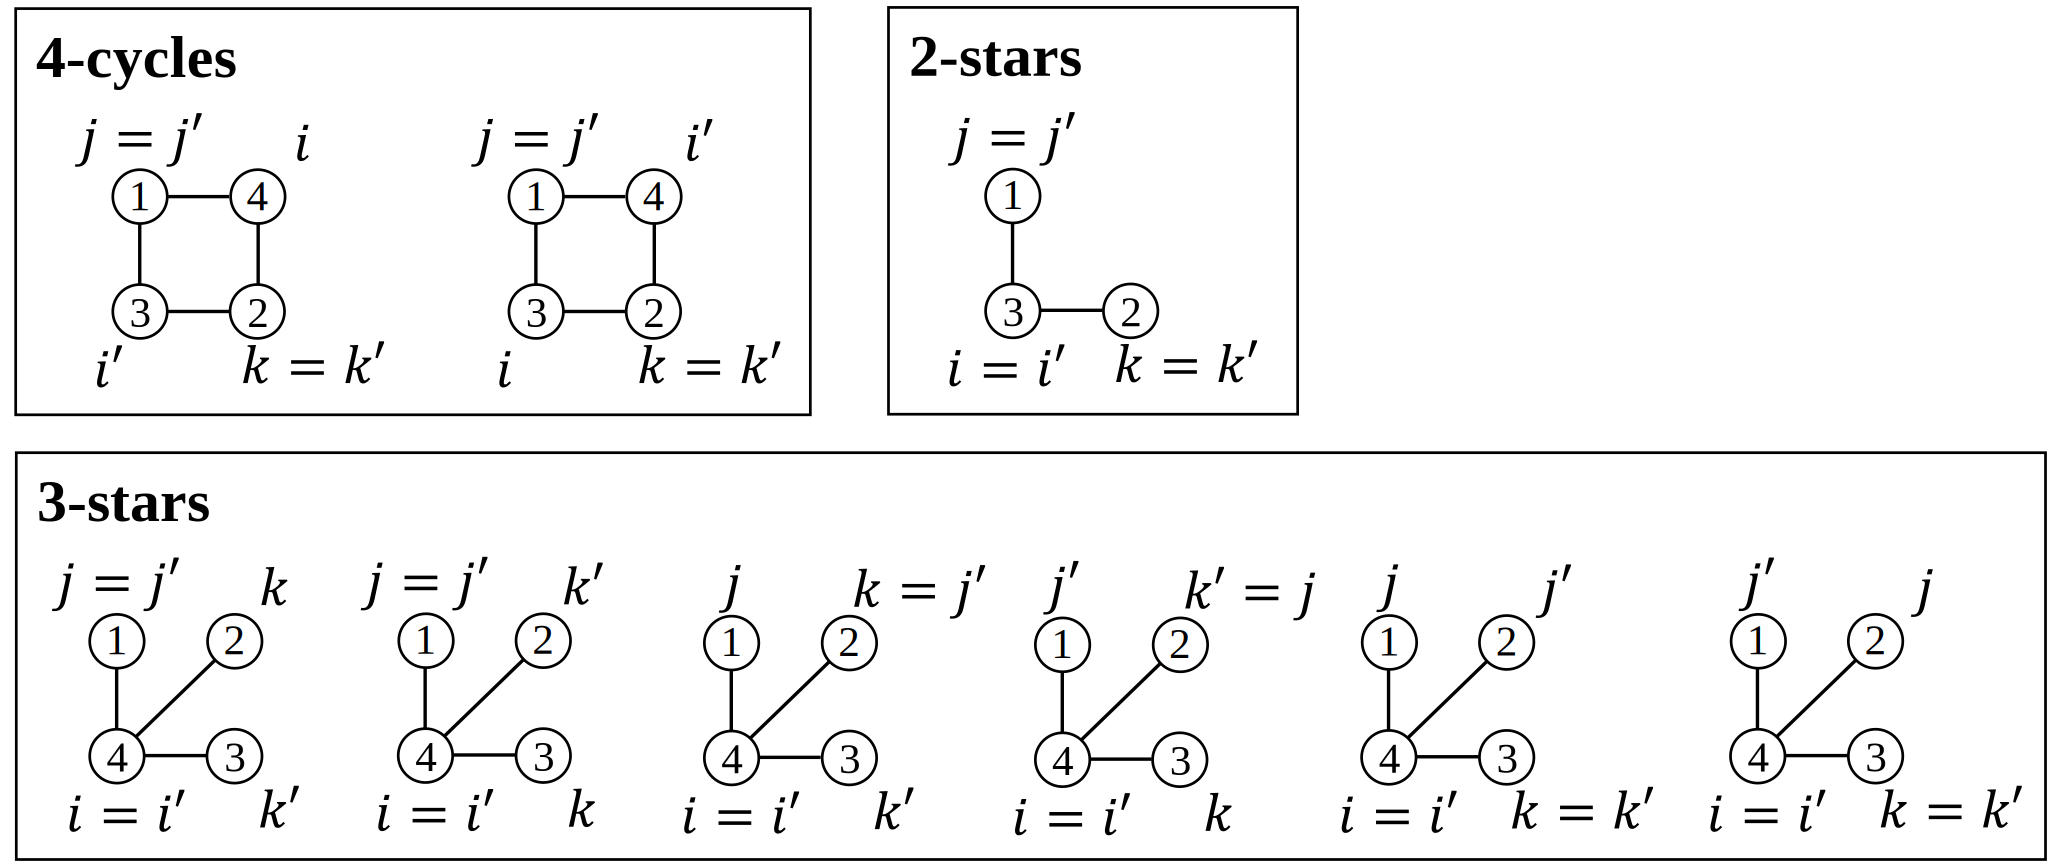
\includegraphics[width=0.99\linewidth]{fig/associated_subgraphs.pdf}
  
  \caption{Examples of two 4-cycles, six 3-stars, and one 2-stars.}
  \label{chap2-fig:associated_subgraphs}
\end{figure}

In the following, let $P(i,j,k)$ be the event that $F_{ijk} = F_{i'j'k'} = 1$.
Observing Figure~\ref{chap2-fig:four-cycle}, we can see that in both possible ways in
which a valid choice maps to a $4$-cycle, then $P(i,j,k)$ holds when at least $3$
edges in $E'$ are present. Each edge in $E'$ is independent,
and is present with probability at most $\mu$. Thus, $\Pr[P(i,j,k)] \leq \mu^3$.
Next, if a valid choice maps to a $3$-star, then $P(i,j,k)$ implies at least $3$
edges in $E'$ are present. Thus, $\Pr[P(i,j,k) = 1] \leq \mu^3$.
Finally, if a valid choice maps to a $2$-star, then $P(i,j,k) = 1$
if and only if $2$ edges in $E'$ are present. Thus, $\Pr[P(i,j,k) = 1] \leq \mu^2$.

Putting this together,
\[
  \V\left[\sum_{i=1}^n w_i\right] \leq 2 C_4(G) \mu^3 + 6 S_3(G) \mu^3 + S_2(G) \mu^2.
\]
Plugging into~\eqref{chap2-eq:inter_var}, we get
% \[
\begin{align*}
  &\;\V[\hf_\triangle(G)] \\
  &\leq \frac{1}{(1-\rho)^2} \left(\frac{1}{\mu}(2C_4(G) + 6S_3(G)) + \frac{1}{\mu^2} S_2(G) + 2n\frac{d_{max}^2}{\mu^4\epsilon_2^2}\right).
% \]
\end{align*}
This establishes the result. \qed

\smallskip
\noindent{\textbf{Bounding the Variance in \AlgThree{}.}}~~In \AlgThree{}, for a fixed
$v_i \in V$, we have $(v_j, v_k) \in M_i$ if and only if
$j < k < i$, $(v_j, v_k) \in E'$, $(v_i, v_k) \in E'$, and $(v_i, v_k) \in E'$
from~\eqref{chap2-eq:M_i_III}. Thus,
\begin{align*}
\sum_{i=1}^n w_i &= \sum_{i=1}^n~\sum_{\substack{1 \leq j < k < i \leq n \\
a_{i,j} = 1, a_{i,k} = 1}} \textbf{1}_{(v_j, v_k) \in M_i} \\
&= \sum_{1 \leq j < k < i \leq n}
a_{i,j}a_{i,k}\textbf{1}_{(v_j, v_k) \in E'} \textbf{1}_{(v_i, v_k) \in E'}\textbf{1}_{(v_j, v_k) \in E'}.
\end{align*}

Define the random variable $F_{ijk} = \textbf{1}_{(v_j v_k) \in E'}
\textbf{1}_{(v_i, v_k) \in E'} \allowbreak \textbf{1}_{(v_j, v_k) \in E'}$. Following the same
steps as those in the proof of \AlgTwo{}, we have
\begin{align*}
  \V\left[\sum_{i=1}^n w_i\right]
  &= \sum_{\substack{1 \leq j < k < i \leq n \\ 1 \leq j' < k' <
  i' \leq n}} a_{i,j} a_{i,k} a_{i',j'} a_{i',k'} \cov(F_{ijk}, F_{i'j'k'}) \\
  &\leq
  \sum_{i,i',j,j',k,k'\text{ valid}} \Pr[F_{ijk} = F_{i'j'k'} = 1].
\end{align*}

As we showed in the proof for \AlgTwo{}, each $4$-cycle of $G$ has at most
2 valid choices mapped to it, each $3$-star of $G$ has at most 6 valid
choices mapped to it, and each $2$-star of $G$ has at most one valid choice
mapped to it.

In the following, let $P(i,j,k)$ be the event that $F_{ijk} = F_{i'j'k'} = 1$.
Observing Figure~\ref{chap2-fig:four-cycle}, we can see that for each possible
mapping of a valid choice to a $4$-cycle, five edges must be present in $G'$ in
order for $P(i,j,k) = 1$. Thus, $\Pr[P(i,j,k) = 1] \leq \mu^5$. For each possible
mapping of a valid choice to a $3$-star, five edges must be present in $G'$ in
order for $P(i,j,k) = 1$. Thus, $\Pr[P(i,j,k) = 1] \leq \mu^5$. For each possible
mapping of a valid choice to a $2$-star, three edges must be present in $G'$ in
order for $P(i,j,k) = 1$. Thus, $\Pr[P(i,j,k) = 1] \leq \mu^3$.

Plugging into~\eqref{chap2-eq:inter_var}, we get
% \[
\begin{align*}
  &\;\V[\hf_\triangle(G)] \\
  &\leq \frac{1}{(1-\rho)^2} \left(\frac{1}{\mu}(2C_4(G) + 6S_3(G)) + \frac{1}{\mu^3} S_2(G) + 2n\frac{d_{max}^2}{\mu^6\epsilon_2^2}\right).
% \]
\end{align*}
This establishes the result.
\qed

\begin{lemma}
  \label{chap2-lem:c_ij_4cycle_2star}
  Let $c_{ij} = \sum_{l < i \leq n} a_{l,i} a_{l,j}$. Then,
\[
    \sum_{i,j=1, i<j}^n c_{ij}^2 \leq 2 C_4(G) + S_2(G).
\]
\end{lemma}
\begin{proof}
  \begin{align*}
      \sum_{i,j=1, i<j}^n c_{ij}^2
      &= \sum_{i,j=1, i<j}^n c_{ij} + \sum_{i,j=1, i<j}^n c_{ij}(c_{ij}-1) \\
      &= S_2(G) + \sum_{i,j=1, i<j}^n c_{ij}(c_{ij}-1).
  \end{align*}
  Let $C_{i-*-j-*-i}(G)$ be the number of 4-cycles in $G$
  %that starts with $i$ and reaches $j$ after two hops.
  such that the first and third nodes are $v_i$ and $v_j$, respectively $(i<j)$, and the remaining two nodes have smaller indices than $i$.
  From middle nodes in 2-paths starting at $v_i$ and ending at $v_j$, we can choose two nodes as the second and fourth nodes in the 4-cycles.
  $c_{ij}$ is the number of nodes that have smaller IDs than $v_i$ and are connected to $v_i$ and $v_j$.
  Thus,
  $C_{i-*-j-*-i}(G) = \binom{c_{ij}}{2}$.
  Therefore, we have
  \begin{align*}
      \sum_{i,j=1, i<j}^n c_{ij}^2
       &= S_2(G) + \sum_{i,j=1, i<j}^n 2C_{i-*-j-*-i}(G) \\
      &\leq S_2(G) + 2 C_4(G).
  \end{align*}
The last inequality comes from the fact that
two nodes with the largest indices may not be opposite to each other in some 4-cycles in $G$.
\end{proof}

\section{Proof of Statements in Section~\ref{chap2-sec:double_clip}}
\label{chap2-sec:proof_double_clip}
\subsection{Proof of Theorem~\ref{chap2-thm:privacy_DC}}

Let $\bma_i, \bma'_i \in \{0,1\}^n$ be two neighbor lists that differ in one bit.
Let ${t_i}'$, $s'_i$, and ${w_i}'$ be respectively the values of $t_i$ (in line 8 of Algorithm~\ref{chap2-alg:clip}), $s_i$ (in line 9), and $w_i$ (in line 10) when the neighbor list of user $v_i$ is $\bma'_i$.
Let $\Delta w_i = |{w_i}' - w_i|$.

We assume that $|\bma'_i| = |\bma_i| + 1$ without loss of generality.
Let $\bar{\bma}_i, \bar{\bma}'_i \in \{0,1\}^n$ be neighbor lists corresponding to $\bma_i$ and $\bma'_i$, respectively, after edge clipping.
Note that $|\bar{\bma}_i| = |\bar{\bma}'_i| \leq \td_i$.
There are three cases for $\bar{\bma}_i$ and $\bar{\bma}'_i$:
\begin{enumerate}
    \item $\bar{\bma}_i$ is identical to $\bar{\bma}'_i$ and $|\bar{\bma}_i| = |\bar{\bma}'_i| = \td_i$.
    \item $\bar{\bma}_i$ and $\bar{\bma}'_i$ differ in one bit and $|\bar{\bma}'_i| = |\bar{\bma}_i| + 1$.
    \item $\bar{\bma}_i$ and $\bar{\bma}'_i$ differ in two bits and $|\bar{\bma}_i| = |\bar{\bma}'_i| = \td_i$.
\end{enumerate}
Note that the third case can happen when $|\bma'_i| \geq \td_i$.
For example, assume that $n=8$, $\td_i=4$, $\bma_i=(1,1,0,1,0,1,1,1)$ and $\bma'_i=(1,1,1,1,0,1,1,1)$.
If we select four ``1''s in the order of 3, 1, 4, 6, 8, 2, 7, and 5-th bit in the neighbor list,
$\bar{\bma}_i$ and $\bar{\bma}'_i$ will be:
$\bar{\bma}_i=(1,0,0,1,0,1,0,1)$ and $\bar{\bma}'_i=(1,0,1,1,0,1,0,0)$,
which differ in two bits.

If $\bar{\bma}_i$ and $\bar{\bma}'_i$ differ in one bit ($|\bar{\bma}'_i| = |\bar{\bma}_i| + 1$), then ${t_i}' - t_i \in [0,\kappa_i]$ and $s'_i - s_i \in [0,\td_i]$, hence $\Delta w_i = |({t_i}' - t_i) - \mu^*\rho(s'_i - s_i)| \leq \kappa_i$.
If $\bar{\bma}_i$ and $\bar{\bma}'_i$ differ in two bits ($|\bar{\bma}_i| = |\bar{\bma}'_i| = d_{max}$), then ${t_i}' - t_i \in [-\kappa_i,\kappa_i]$ and $s_i = s'_i = \binom{\td_i}{2}$, hence $\Delta w_i \leq \kappa_i$.

Therefore, we always have $\Delta w_i \leq \kappa_i$
(if $\bar{\bma}_i$ is identical to $\bar{\bma}'_i$, $\Delta w_i =0$).
Since we add $\Lap(\frac{1}{\epsilon_0})$
to $d_i$ and
$\Lap(\frac{\kappa_i}{\epsilon_2})$
to $w_i^*$, the second round provides ($\epsilon_0+\epsilon_2$)-edge LDP.
The first round provides $\epsilon_1$-edge LDP and we use only the lower-triangular part of $\bmA$.
Thus, by sequential composition (Proposition~\ref{chap2-prop:seq_comp_edge_LDP}) 
and Proposition~\ref{chap2-prop:edge_LDP_entire_edge_LDP},
$\calR_i$ satisfies $(\epsilon_0 + \epsilon_1 + \epsilon_2)$-edge LDP, and $(\calR_1, \ldots, \calR_n)$ satisfies $(\epsilon_0 + \epsilon_1 + \epsilon_2)$-relationship DP.
\qed

\subsection{Proof of Theorem~\ref{chap2-thm:triangle_excess}}

Recall that
$t_{i,j} = |\{(v_i,v_j,v_k) : a_{i,k} = 1, (v_j,v_k) \in M_i, j<k<i \}|$.
Let
$t'_{i,j} = |\{(v_i,v_j,v_k) : a_{i,k} = 1, (v_j,v_k) \in M_i \}|$.
Then $t_{i,j} \leq t'_{i,j}$.
Thus we have
\begin{align*}
    \Pr(t_{i,j} > \kappa_i) \leq \Pr(t_{i,j} \geq \kappa_i) \leq \Pr(t'_{i,j} \geq \kappa_i).
\end{align*}

Below we first prove (\ref{chap2-eq:AlgI_clip_bound}) and (\ref{chap2-eq:AlgII_clip_bound}). Then we prove (\ref{chap2-eq:AlgIII_clip_bound}).

\smallskip
\noindent{\textbf{Proof of (\ref{chap2-eq:AlgI_clip_bound}) and (\ref{chap2-eq:AlgII_clip_bound}).}}~~For each edge $(v_i,v_j)$, we have $\sum_{k \ne i,j} \textbf{1}_{(v_i,v_k) \in E} \leq \td_i$.
% In addition, each edge $(v_j,v_k)$ is included in $E'$ with probability at most $\mu^*$, and all the events are independent in \AlgOne{} and \AlgTwo{}.
In \AlgOne{}, each edge $(v_j,v_k)$ is included in $E'$ with probability at most $\mu$, and all the events are independent.
In \AlgTwo{}, each of the edges $(v_i,v_k)$ and $(v_j,v_k)$ is included in $E'$ with probability at most $\mu$, and all the events are independent.
Thus, $\Pr(t'_{i,j} \geq \kappa_i)$ is less than or equal to the probability that the number of successes in the binomial distribution $B(\td_i, \mu^*)$ ($\mu^* = \mu$ in \AlgOne{} and $\mu^2$ in \AlgTwo{}) is larger than or equal to $\kappa_i$.

Let $X_{n,p}$ be a random variable representing the number of successes in the binomial distribution $B(n,p)$, and $F(\kappa_i;n,p) = \Pr(X_{n,p} \leq \kappa_i)$; i.e., $F$ is a cumulative distribution function of $B(n,p)$.
Since $\kappa_i \geq \mu^* \td_i$, we have
\begin{align*}
    &\Pr(t'_{i,j} \geq \kappa_i) \\
    &\leq \Pr(X_{\td_i, \mu^*} \geq \kappa_i) \\
    &= F(\td_i - \kappa_i; \td_i, 1-\mu^*) \\
    &\leq \exp \left[-\td_i D \left(\frac{\td_i - \kappa_i}{\td_i} \parallel 1-\mu^* \right) \right]  \text{(by Chernoff bound)}\\
    &= \exp \left[-\td_i D \left(\frac{\kappa_i}{\td_i} \parallel \mu^* \right) \right],
\end{align*}
which proves (\ref{chap2-eq:AlgI_clip_bound}) and (\ref{chap2-eq:AlgII_clip_bound}) (as $\Pr(t_{i,j} > \kappa_i) \leq \Pr(t'_{i,j} \geq \kappa_i)$).

\smallskip
\noindent{\textbf{Proof of (\ref{chap2-eq:AlgIII_clip_bound}).}}~~Assume that $\kappa_i \geq \mu^2 \td_i$ in \AlgThree{}.
For each edge $(v_i,v_j)$, we have $\sum_{k \ne i,j} \textbf{1}_{(i,k) \in E} \leq \td_i$.
In addition, each of the edges $(v_i,v_k)$ and
$(v_j,v_k)$ are included in $E'$ with probability at most $\mu$, and all the events are independent.

If $(v_i,v_j)$ is included in $E'$ (which happens with probability at most $\mu$), $\Pr(t'_{i,j} \geq \kappa_i)$ is less than or equal to the probability that the number of successes in the binomial distribution $B(\td_i, \mu^2)$ is larger than or equal to $\kappa_i$.
Otherwise (i.e., if $(v_i,v_j)$ is not included in $E'$), then $t'_{i,j} = 0$.

Thus, if $\kappa_i \geq \mu^2 \td_i$, we have
\begin{align*}
    &\Pr(t'_{i,j} \geq \kappa_i) \\
    &\leq \mu \Pr(X_{\td_i, \mu^2} \geq \kappa_i) \\
    &= \mu F(\td_i - \kappa_i; \td_i, 1-\mu^2) \\
    &\leq \mu \exp \left[-\td_i D \left(\frac{\td_i - \kappa_i}{\td_i} \parallel 1-\mu^2 \right) \right]  ~ \text{(by Chernoff bound)}\\
    &= \mu \exp \left[-\td_i D \left(\frac{\kappa_i}{\td_i} \parallel \mu^2 \right) \right],
\end{align*}
and therefore (\ref{chap2-eq:AlgIII_clip_bound}) holds (as $\Pr(t_{i,j} > \kappa_i) \leq \Pr(t'_{i,j} \geq \kappa_i)$).


If $\mu^3 \td_i \leq \kappa_i < \mu^2 \td_i$, (\ref{chap2-eq:AlgIII_clip_bound}) can be written as: $\Pr(t_{i,j} > \kappa_i) \leq \mu \exp \left[-\td_i D \left(\mu^2 \parallel \mu^2 \right) \right] = \mu$.
This clearly holds because each edge $(v_i,v_j)$ is included in $E'$ with probability at most $\mu$.
\qed
}


%%%%%%%%%%%%%%%%%%%%%%%%%%%%%%%%%%%%%%%%%%%%%%%%%%%%%%%%%%%%%%%%%%%%%%%%%%%%%%%%
\end{document}
%%%%%%%%%%%%%%%%%%%%%%%%%%%%%%%%%%%%%%%%%%%%%%%%%%%%%%%%%%%%%%%%%%%%%%%%%%%%%%%%
